% see http://hal.inria.fr/hal-00934443 to simplify/improve the ulp calculus

\documentclass[12pt]{amsart}

\usepackage{fullpage}
\usepackage{amssymb}
\usepackage{amsmath}
\usepackage{url}
\usepackage{comment}
\usepackage{hyperref}
\usepackage{graphicx}

\pagestyle{plain}
\title{The MPFR\footnote{\lowercase{\url{http://www.mpfr.org/}}} Library:
Algorithms and Proofs}
\author{The MPFR team}

%%%%%%%%%%%%%% macros for the package algorithm2e %%%%%%%%%%%%%%%
\usepackage[english, lined, linesnumbered]{algorithm2e}
\SetKwData{tempv}{temp}
\SetKwData{tzero}{t0}
\SetKwData{tone}{t1}
\SetKwData{ivar}{i}
\SetKwData{kvar}{k}
\SetKwData{svar}{s}
\SetKwData{approxErr}{approxErr}
\SetKwData{evalErr}{evalErr}
\SetKwData{correctBits}{correctBits}
\SetKwData{wprec}{wprec}
\SetKwData{precc}{prec}
\SetKwData{cond}{cond}
\SetKwData{assumedExp}{assumedExp}
%%%%%%%%%%%%%%%%%%%%%%%%%%%%%%%%%%%%%%%%%%%%%%%%%%%%%%%%%%%%%%%%%

\DeclareMathOperator{\Ai}{Ai}
\DeclareMathOperator{\acosh}{acosh}
\DeclareMathOperator{\Li2}{Li_2}
\DeclareMathOperator{\erf}{erf}
\DeclareMathOperator{\erfc}{erfc}

\def\O{{\mathcal O}}
\def\n{\textnormal}
\def\pinf{\bigtriangleup}
\def\minf{\bigtriangledown}
\def\q{\hspace*{5mm}}
\def\ulp{{\rm ulp}}
\def\Exp{{\rm \textsc exp}}
\def\prec{{\rm prec}}
\def\sign{{\rm sign}}
\def\Paragraph#1{\noindent {\sc #1}}
\def\Z{{\mathcal Z}}
\def\Q{{\mathbb Q}}
\def\R{{\mathbb R}}
\def\C{{\mathbb C}}
\def\N{{\mathcal N}}
\def\If{{\bf if}}
\def\then{{\bf then}}
\def\Else{{\bf else}}
\def\elif{{\bf elif}}
\def\for{{\bf for}}
\def\to{{\bf to}}
\def\while{{\bf while}}
\def\err{{\rm err}}
\def\cmod{\,\mathrm{cmod}\,}

\newcommand{\U}[1]{\quad \mbox{[Rule~\ref{#1}]}}
\newcommand{\fl}[1]{\widehat{#1}}
\newcommand{\rnd}[1]{\left\langle#1\right\rangle}

\DeclareMathOperator{\error}{error}

\newtheorem{Rule}{Rule}
\newtheorem{lemma}{Lemma}
\newtheorem{theorem}{Theorem}
\newtheorem{fact}{Fact}
\newtheorem{assumption}{Hypothesis}

\begin{document}
\maketitle
\sloppy

\tableofcontents

\section{Notations and Assumptions}

In the whole document, $\N()$ denotes rounding to nearest,
$\Z()$ rounding toward zero,
$\pinf()$ rounding toward plus infinity,
$\minf()$ rounding toward minus infinity,
and $\circ()$ any of those four rounding modes.

In the whole document, except special notice, all variables are assumed
to have the same precision, usually denoted $p$.

\section{Error calculus}

Let $n$ --- the working precision ---
be a positive integer (considered fixed in the following).
We write any nonzero real number $x$ in the form $x = m \cdot 2^e$
with $\frac{1}{2} \le |m| < 1$ and $e := \Exp(x)$, and
we define $\ulp(x) := 2^{\Exp(x) - n}$.

\subsection{Ulp calculus}

\begin{Rule} \label{R1}
$2^{-n} |x| < \ulp(x) \le 2^{-n+1} |x|$.
\end{Rule}
\begin{proof}
Obvious from $x = m \cdot 2^e$ with $\frac{1}{2} \le |m| < 1$.
\end{proof}

\begin{Rule} \label{R2}
If $a$ and $b$ have same precision $n$,
and $|a| \le |b|$, then $\ulp(a) \le \ulp(b)$.
\end{Rule}
\begin{proof}
Write $a = m_a \cdot 2^{e_a}$ and $b = m_b \cdot 2^{e_b}$.
Then $|a| \le |b|$ implies $e_a \le e_b$, thus
$\ulp(a) = 2^{e_a-n} \le 2^{e_b-n} = \ulp(b)$.
\end{proof}

\begin{Rule} \label{R3}
Let $x$ be a real number, and $y = \circ(x)$.
Then $|x - y| \leq \frac{1}{2} {\rm min}(\ulp(x), \ulp(y))$
in rounding to nearest,
and $|x - y| \leq {\rm min}(\ulp(x), \ulp(y))$ for the other rounding modes.
\end{Rule}
\begin{proof}
First consider rounding to nearest.
By definition, we have $|x-y| \leq \frac{1}{2} \ulp(y)$.
If $\ulp(y) \leq \ulp(x)$, then $|x-y| \leq \frac{1}{2} \ulp(y)
\leq \frac{1}{2} \ulp(x)$.
The only difficult case is when $\ulp(x) < \ulp(y)$, but then
necessarily $y$ is a power of two;
since in that case $y - \frac{1}{2} \ulp(y)$ is exactly representable,
the maximal possible difference between $x$ and $y$
is $\frac{1}{4} \ulp(y) = \frac{1}{2} \ulp(x)$, which concludes the proof
in the rounding to nearest case.

In rounding to zero, we always have $\ulp(y) \leq \ulp(x)$, so the rule
holds.
In rounding away from zero, the only difficult case is when
$\ulp(x) < \ulp(y)$, but then $y$ is a power of two, and since
$y - \frac{1}{2} \ulp(y)$ is exactly representable,
the maximal possible difference between $x$ and $y$ is $\frac{1}{2} \ulp(y)
= \ulp(x)$, which concludes the proof.
\end{proof}

\begin{Rule} \label{R4}
$\frac{1}{2} |a| \cdot \ulp(b) < \ulp(a b) < 2 |a| \cdot \ulp(b)$.
\end{Rule}
\begin{proof}
Write $a = m_a 2^{e_a}$, $b = m_b \cdot 2^{e_b}$, and $a b = m 2^e$
with $\frac{1}{2} \le m_a, m_b, m < 1$,
then $\frac{1}{4} 2^{e_a+e_b} \le |a b| < 2^{e_a+e_b}$,
thus $e = e_a + e_b$ or $e = e_a + e_b - 1$, which implies
$\frac{1}{2} 2^{e_a} \ulp(b) \le \ulp(a b) \le 2^{e_a} \ulp(b)$
using $2^{e_b-n} = \ulp(b)$, and the rule follows from
the fact that $|a| < 2^{e_a} \le 2|a|$ (equality on the right side can
occur only if $e = e_a + e_b$ and $m_a = \frac{1}{2}$, which are
incompatible).
\end{proof}

\begin{Rule} \label{R5}
$\ulp(2^k a) = 2^k \ulp(a)$.
\end{Rule}
\begin{proof}
Easy: if $a = m_a \cdot 2^{e_a}$, then $2^k a = m_a \cdot 2^{e_a+k}$.
\end{proof}

\begin{Rule} \label{R6}
Let $x > 0$, $\circ(\cdot)$ be any rounding, and $u := \circ(x)$,
then $\frac{1}{2} u < x < 2 u$.
\end{Rule}
\begin{proof}
Assume $x \geq 2 u$, then $2u$ is another representable number which is closer
from $x$ than $u$, which leads to a contradiction. The same argument proves
$\frac{1}{2} u < x$.
\end{proof}

\begin{Rule} \label{R7}
$\frac{1}{2} |a| \cdot \ulp(1) < \ulp(a) \leq |a| \cdot \ulp(1)$.
\end{Rule}
\begin{proof}
The left inequality comes from Rule~\ref{R4} with $b=1$,
and the right one from $|a| \ulp(1) \geq \frac{1}{2} 2^{e_a} 2^{1-n} =\ulp(a)$.
\end{proof}

\begin{Rule} \label{R8}
For any $x \neq 0$ and any rounding mode $\circ(\cdot)$,
we have $\ulp(x) \leq \ulp(\circ(x))$, and equality holds when rounding toward
zero, toward $-\infty$ for $x>0$, or toward $+\infty$ for $x<0$.
\end{Rule}
\begin{proof}
Without loss of generality, assume $x > 0$.
Let $x = m \cdot 2^e$ with $\frac{1}{2} \leq m < 1$.
As $\frac{1}{2} 2^{e_x}$ is a machine number, necessarily $\circ(x) \geq
\frac{1}{2} 2^{e_x}$, thus by Rule~\ref{R2}, then $\ulp(\circ(x)) \geq
2^{e_x - n} = \ulp(x)$.
If we round toward zero, then $\circ(x) \leq x$ and by Rule~\ref{R2} again,
$\ulp(\circ(x)) \leq \ulp(x)$.
\end{proof}

\begin{Rule} \label{R9}
\begin{eqnarray}\nonumber
&&\n{For}\;\;  \error(u) \leq k_u \ulp(u),\;\; u.c_u^- \leq x \leq u.c_u^+\\\nonumber
&&\n{with}\;\;   c_u^{-}=1- k_u 2^{1-p} \n{ and } c_u^{+}=1+ k_u 2^{1-p}
\end{eqnarray}

\begin{eqnarray}\nonumber
&&\n{For}\;\;  u=\circ(x),\;\; u.c_u^- \leq x \leq u.c_u^+\\\nonumber
&&\n{if}\;\;  u=\pinf(x),\n{ then } c_u^+=1\\\nonumber
&&\n{if}\;\;  u=\minf(x),\n{ then } c_u^-=1\\\nonumber
&&\n{if}\;\;  \n{for $x<0$ and } u=\Z(x),\n{ then } c_u^+=1 \\\nonumber
&&\n{if}\;\;  \n{for $x>0$ and } u=\Z(x),\n{ then } c_u^-=1 \\\nonumber
&&\n{else}\;\;   c_u^{-}=1-2^{1-p} \n{ and } c_u^{+}=1+2^{1-p}
\end{eqnarray}
\end{Rule}

\subsection{Relative error analysis}

Another way to get a bound on the error,
is to bound the relative error. This is sometimes easier than using the
``ulp calculus'' especially when performing only multiplications or divisions.

\begin{Rule} \label{R10}
If $u := \circ_p(x)$, then we can write both:
\[ u = x (1 + \theta_1), \qquad x = u (1 + \theta_2), \]
where $|\theta_i| \leq 2^{-p}$ for rounding to nearest, and
$|\theta_i| < 2^{1-p}$ for directed rounding.
\end{Rule}
\begin{proof}
This is a simple consequence of Rule~\ref{R3}. For rounding to nearest,
we have $|u-x| \leq \frac{1}{2} \ulp(t)$ for $t=u$ or $t=x$, hence by
Rule~\ref{R1} $|u-x| \leq 2^{-p}$.
\end{proof}

\begin{Rule} \label{R11}
Assume $x_1, \ldots, x_n$ are $n$ floating-point numbers in precision $p$,
and we compute an approximation of their product with the following sequence
of operations: $u_1 = x_1, u_2 = \circ(u_1 x_2), \ldots, u_n = \circ(u_{n-1}
x_n)$. If rounding away from zero, the total rounding error is bounded by
$2(n-1) \ulp(u_n)$.
\end{Rule}
\begin{proof}
We can write $u_1 x_2 = u_2 (1 - \theta_2), \ldots, u_{n-1} x_n = u_n
(1 - \theta_n)$, where $0 \leq \theta_i \leq 2^{1-p}$.
We get $x_1 x_2 \ldots x_n = u_n (1 - \theta_2) \ldots (1 - \theta_n)$,
which we can write $u_n (1-\theta)^{n-1}$ for some $0 \leq \theta \leq 2^{1-p}$
by the intermediate value theorem.
Since $1-nt \leq (1-t)^n \leq 1$, we get $|x_1 x_2 \ldots x_n - u_n| \leq
(n-1) 2^{1-p} |u_n| \leq 2 (n-1) \ulp(u_n)$ by Rule~\ref{R1}.
\end{proof}

% \section{Generic error on basic operations}

\subsection{Generic error of addition/subtraction}\label{generic:sous}

We want to compute the generic error of the subtraction, the following rules
apply to addition too.

\begin{eqnarray}\nonumber
\textnormal{Note:}&& \error(u) \leq k_u \, \ulp(u), \;\; \error(v) \leq k_v \, \ulp(v)
\end{eqnarray}

\begin{eqnarray}\nonumber
\textnormal{Note:}&& \ulp(w)=2^{e_w-p}, \;\; \ulp(u)=2^{e_u-p},\;\; \ulp(v)=2^{e_v-p}\;\;\textnormal{with} \; p \; \textnormal{the precision} \\\nonumber
&& \ulp(u)=2^{d+e_w-p}, \;\; \ulp(v)=2^{d^{'}+e_w-p},\;\;\textnormal{with} \;\;d=e_u-e_w \;\; d^{'}=e_v-e_w
\end{eqnarray}
\begin{eqnarray}\nonumber
\error(w)& \leq &c_w \ulp(w) + k_u \ulp(u) + k_v \ulp(v) \\\nonumber
&=&(c_w+k_u 2^d+ k_v 2^{d^{'}}) \ulp(w)
\end{eqnarray}
\begin{eqnarray}\nonumber
&&\textnormal{If} \;\; ( u \geq 0  \;\;\textnormal{and}\;\;  v \geq 0) \;\;\textnormal{or}\;\; (u \leq 0 \;\;\textnormal{and}\;\; v \leq 0)
\end{eqnarray}
\begin{eqnarray}\nonumber
\error(w)& \leq&(c_w + k_u + k_v) \, \ulp(w)
\end{eqnarray}
\begin{eqnarray}\nonumber
\textnormal{Note:}&&\textnormal{If}\;\; w=\N(u+v) \;\;\textnormal{Then}\;\; c_w =\frac{1}{2} \;\;\textnormal{else}\;\; c_w =1\\\nonumber
\end{eqnarray}

\subsection{Generic error of multiplication}\label{generic:mul}

We want to compute the generic error of the multiplication.
We assume here $u, v > 0$ are approximations of exact values respectively $x$
and $y$, with $|u - x| \leq k_u \, \ulp(u)$ and $|v - y| \leq k_v \, \ulp(v)$.

\begin{eqnarray}\nonumber
w&=&\circ(uv) \\\nonumber
% \textnormal{Note:}&& \error(u) \leq k_u \, \ulp(u), \;\; \error(v) \leq k_v \, \ulp(v)
\end{eqnarray}
\begin{eqnarray}\nonumber
\error(w)& = &|w - xy| \\\nonumber
& \leq &|w - u v| +|u v - x y| \\\nonumber
& \leq & c_w \ulp(w) +  \frac{1}{2} [|u v-u y|+|u y-x y|+|u v-x v|+|x v-x y|]\\\nonumber
& \leq & c_w \ulp(w) +  \frac{u+x}{2} k_v \ulp(v) + \frac{v+y}{2} k_u \ulp(u)\\\nonumber
& \leq & c_w \ulp(w) +  \frac{u(1+c_u^+)}{2} k_v \ulp(v) + \frac{v(1+c_v^+)}{2} k_u \ulp(u) \U{R9}\\\nonumber
& \leq & c_w \ulp(w) +  (1+c_u^+) k_v \ulp(uv) + (1+c_v^+) k_u \ulp(uv) \U{R4}\\\nonumber
& \leq & [ c_w +  (1+c_u^+) k_v + (1+c_v^+) k_u ] \ulp(w)\U{R8}\\\nonumber
\end{eqnarray}
\begin{eqnarray}\nonumber
\textnormal{Note:}&&\textnormal{If}\;\; w=\N(uv) \;\;\textnormal{Then}\;\; c_w =\frac{1}{2} \;\;\textnormal{else}\;\; c_w =1
\end{eqnarray}

\subsection{Generic error of inverse}\label{generic:inv}

We want to compute the generic error of the inverse.
We assume $u > 0$.

\begin{eqnarray}\nonumber
w&=&\circ(\frac{1}{u}) \\\nonumber
\textnormal{Note:}&& \error(u) \leq k_u \, \ulp(u)
\end{eqnarray}
\begin{eqnarray}\nonumber
\error(w)& = &|w - \frac{1}{x}| \\\nonumber
& \leq &|w - \frac{1}{u}| +|\frac{1}{u} - \frac{1}{x}| \\\nonumber
& \leq & c_w \ulp(w) + \frac{1}{ux}|u-x| \\\nonumber
& \leq & c_w \ulp(w) + \frac{k_u}{ux} \ulp(u)
\end{eqnarray}
\begin{eqnarray}\nonumber
\textnormal{Note:}&& \frac{u}{c_u} \leq x\;\; \U{R6}\\\nonumber
&&\n{for } u=\minf(x),\;c_u=1 \n{ else } c_u=2\\\nonumber
&& \n{then: } \frac{1}{x} \leq c_u \frac{1}{u}
\end{eqnarray}
\begin{eqnarray}\nonumber
\error(w)& \leq & c_w \ulp(w) + c_u\frac{k_u}{u^2} \ulp(u)\\\nonumber
& \leq & c_w \ulp(w) + 2.c_u.k_u \ulp(\frac{u}{u^2}) \U{R4}\\\nonumber
& \leq & [c_w + 2.c_u.k_u].\ulp(w) \U{R8}
\end{eqnarray}
\begin{eqnarray}\nonumber
\textnormal{Note:}&&\textnormal{If}\;\; w=\N(\frac{1}{u}) \;\;\textnormal{Then}\;\; c_w =\frac{1}{2} \;\;\textnormal{else}\;\; c_w =1\\\nonumber\end{eqnarray}

\subsection{Generic error of division}\label{generic:div}


We want to compute the generic error of the division.
Without loss of generality, we assume all variables are positive.
\begin{eqnarray}\nonumber
w&=&\circ(\frac{u}{v}) \\\nonumber
\textnormal{Note:}&& \error(u) \leq k_u \, \ulp(u), \;\; \error(v) \leq k_v \, \ulp(v)
\end{eqnarray}
\begin{eqnarray}\nonumber
\error(w)& = &|w - \frac{x}{y}| \\\nonumber
& \leq &|w - \frac{u}{v}| +|\frac{u}{v} - \frac{x}{y}| \\\nonumber
& \leq & c_w \ulp(w) + \frac{1}{vy}|uy-vx| \\\nonumber
& \leq & c_w \ulp(w) + \frac{1}{vy}[|uy-xy|+|xy-vx| ]\\\nonumber
& \leq & c_w \ulp(w) + \frac{1}{vy}[y k_u \ulp(u)+ x k_v \ulp(v)]\\\nonumber
&   =  & c_w \ulp(w) + \frac{k_u}{v}  \ulp(u)+ \frac{k_v x}{vy} \ulp(v)
\end{eqnarray}
\begin{eqnarray}\nonumber
\textnormal{Note:}&& \frac{\ulp(u)}{v} \leq  2 \ulp(\frac{u}{v}) \;\; \U{R4}\\\nonumber
&& 2 \ulp(\frac{u}{v}) \leq  2 \ulp(w) \;\; \U{R8}
\end{eqnarray}
\begin{eqnarray}\nonumber
\textnormal{Note:}&& x \leq c_u u \textnormal{ and } \frac{v}{c_v} \leq y\;\; \U{R6}\\\nonumber
&&\n{with } \n{for } u=\pinf(x),\;c_u=1 \n{ else } c_u=2\\\nonumber
&&\n{ and }\n{for } v=\minf(y),\;c_v=1 \n{ else } c_v=2\\\nonumber
&& \n{then: } \frac{x}{y} \leq c_u c_v  \frac{u}{v}
\end{eqnarray}
\begin{eqnarray}\nonumber
\error(w)& \leq & c_w \ulp(w) + 2.k_u  \ulp(w)+ c_u.c_v.\frac{k_v u}{vv} \ulp(v)\\\nonumber
& \leq & c_w \ulp(w) + 2.k_u  \ulp(w)+ 2.c_u.c_v.k_v \ulp(\frac{u.v}{v.v}) \U{R4}\\\nonumber
& \leq & [c_w  + 2.k_u+ 2.c_u.c_v.k_v].\ulp(w) \U{R8}
\end{eqnarray}
\begin{eqnarray}\nonumber
\textnormal{Note:}&&\textnormal{If}\;\; w=\N(\frac{u}{v}) \;\;\textnormal{Then}\;\; c_w =\frac{1}{2} \;\;\textnormal{else}\;\; c_w =1
\end{eqnarray}
Note that we can obtain a slightly different result by writing
$uy-vx = (uy - uv) + (uv - vx)$ instead of $(uy-xy)+(xy-vx)$.

Another result can be obtained using a relative error analysis.
Assume $x = u (1 + \theta_u)$ and $y = v (1 + \theta_v)$. Then
$|\frac{u}{v} - \frac{x}{y}| \leq \frac{1}{vy} |uy - uv|
+ \frac{1}{vy} |uv - xv|
= \frac{u}{y} (|\theta_u|+|\theta_v|)$.
If $v \leq y$ and $\frac{u}{v} \leq w$,
this is bounded by $w (|\theta_u|+|\theta_v|)$.

\subsection{Generic error of square root}\label{generic:sqrt}


We want to compute the generic error of the square root of a floating-point
number $u$, itself an approximation to a real $x$,
with $|u - x| \leq k_u \ulp(u)$.
If $v = \circ(\sqrt{u})$, then:
\begin{eqnarray}\nonumber
\error(v) := |v - \sqrt{x}|
& \leq &|v - \sqrt{u}| +|\sqrt{u} - \sqrt{x}| \\\nonumber
& \leq & c_v \ulp(v) + \frac{1}{\sqrt{u} + \sqrt{x}}|u-x| \\\nonumber
& \leq & c_v \ulp(v) + \frac{1}{\sqrt{u} + \sqrt{x}} k_u \ulp(u) \\\nonumber
\end{eqnarray}
Since by Rule~\ref{R9} we have $u.c_u^- \leq x$,
it follows $\frac{1}{\sqrt{x}+\sqrt{u}} \leq
        \frac{1}{\sqrt{u}.(1+\sqrt{c_u^-})}$:
\begin{eqnarray}\nonumber
\error(v)& \leq & c_v \ulp(v) +
                 \frac{1}{\sqrt{u}.(1+\sqrt{c_u^-})}  k_u \ulp(u) \\\nonumber
& \leq & c_v \ulp(v) + \frac{2}{1+\sqrt{c_u^-}}
       k_u \ulp(\sqrt{u}) \;\; \U{R4}\\\nonumber
& \leq & (c_v + \frac{2k_u}{1+\sqrt{c_u^-}})  \ulp(v). \;\; \U{R8}\\\nonumber
\end{eqnarray}
If $u$ is less than $x$, we have $c_u^-=1$ and
we get the simpler formula
$|v-\sqrt{x}| \leq (c_v + k_u)  \ulp(v)$.

\subsection{Generic error of the exponential }\label{generic:exp}


We want to compute the generic error of the exponential.

\begin{eqnarray}\nonumber
v&=&\circ(e^{u}) \\\nonumber
\textnormal{Note:}&& \error(u) \leq k_u \, \ulp(u)\\\nonumber
\end{eqnarray}
\begin{eqnarray}\nonumber
\error(v)& = &|v - e^{x}| \\\nonumber
& \leq &|v - e^{u}| +|e^{u} - e^{x}| \\\nonumber
& \leq & c_v \ulp(v) +  e^t |u-x| \n{ with Rolle's theorem, for } t\in[x,u]\n{ or }t\in[u,x]
\end{eqnarray}
\begin{eqnarray}\nonumber
\error(v)& \leq & c_v \ulp(v) +  c_u^* e^u k_u \ulp(u) \\\nonumber
& \leq & c_v \ulp(v) +  2 c_u^* u k_u \ulp(e^u) \;\U{R4}\\\nonumber
& \leq & (c_v +  2 c_u^* u k_u )\ulp(v) \;\U{R8}\\\nonumber
& \leq & (c_v +  c_u^* 2^{\Exp(u)+1} k_u )\ulp(v)
\end{eqnarray}
\begin{eqnarray}\nonumber
\textnormal{Note:}&& u= m_u 2^{e_u} \n{ and }\ulp(u)=2^{e_u-p} \n{ with } p \n{ the precision} \\\nonumber
\n{ Case }&x \leq u&  c_u^* =1 \\\nonumber
\n{ Case }&u \leq x& \\\nonumber
&&  x \leq u + k_u \ulp(u)\\\nonumber
&& e^x \leq e^u e^{k_u \ulp(u)}\\\nonumber
&&e^x \leq e^u e^{k_u 2^{e_u-p}}\\\nonumber
&\n{then}& c_u^* = e^{k_u 2^{\Exp(u)-p}}\\\nonumber
\end{eqnarray}

\subsection{Generic error of the logarithm}\label{generic:log}
Assume $x$ and $u$ are positive values,
with $|u - x| \leq k_u \ulp(u)$.
We additionally assume $u \leq 4x$. Let $v = \circ(\log u)$.
\begin{eqnarray}\nonumber
\error(v)& = &|v - \log x|
  \leq |v - \log u| +|\log u - \log x| \\\nonumber
& \leq & c_v \ulp(v) + |\log\frac{x}{u}|
  \leq   c_v \ulp(v) + 2 \frac{|x-u|}{u} \\\nonumber
& \leq & c_v \ulp(v) + \frac{2 k_u \, \ulp(u)}{u}
  \leq   c_v \ulp(v) + 2 k_u \, \ulp(1)\;\; \U{R7}\\\nonumber
& \leq & c_v \ulp(v) + 2 k_u \, 2^{1-e_v} \ulp(v)
  \leq   (c_v + k_u 2^{2-e_v}) \ulp(v).
\end{eqnarray}
We used at line 2 the inequality $|\log t| \leq 2 |t-1|$ which holds
for $t \geq \rho$, where $\rho \approx 0.203$ satisfies $\log \rho =2(\rho-1)$.
At line 4, $e_v$ stands for the exponent of $v$, i.e,
$v = m \cdot 2^{e_v}$ with $1/2 \leq |m| < 1$.

\subsection{Ulp calculus vs relative error}

The error in ulp (ulp-error) and the relative error are related as follows.

Let $n$ be the working precision.
Consider $u = \circ(x)$, then the error on $u$ is at most
$\ulp(u) = 2^{\Exp(u)-n} \leq |u| \cdot 2^{1-n}$, thus the relative error
is $\leq 2^{1-n}$.

Respectively, if the relative error is $\leq \delta$, then the error
is at most $\delta |u| \leq \delta 2^n \ulp(u)$. (Going from the ulp-error
to the relative error and back, we lose a factor of two.)

It is sometimes more convenient to use the relative error instead of the
error in ulp (ulp-error), in particular when only multiplications or
divisions are made.
In that case,
Higham \cite{Higham02} proposes the following framework:
we associate to each variable the cumulated number $k$ of roundings that were
made.
The $i$th rounding introduces a relative error of $\delta_i$,
with $|\delta_i| \leq 2^{1-n}$, i.e. the computed result is
$1+\delta_i$ times the exact result.
Hence $k$ successive roundings give a error factor of $(1+\delta_1)
(1+\delta_2) \cdots (1+\delta_k)$, which is between $(1-\varepsilon)^k$
and $(1+\varepsilon)^k$ with $\varepsilon = 2^{1-n}$.
In particular, if all roundings are away, the final relative error is
at most $k \varepsilon = k \cdot 2^{1-n}$, thus at most $2k$ ulps.

\begin{lemma} \label{rel_ulp}
If a value is computed by $k$ successive multiplications or divisions,
each with rounding away from zero, and precision $n$, then the final
error is bounded by $2k$ ulps.
\end{lemma}

If the rounding are not away from zero, the following lemma is still useful
% \cite{Graillat05}:
\cite[Lemma 3.1]{Higham02}:
\begin{lemma} \label{lemma_graillat}
Let $\delta_1, \ldots, \delta_n$ be $n$ real values such that
$|\delta_i| \leq \epsilon$, for $n \epsilon < 1$.
Then we can write $\prod_{i=1}^n (1+\delta_i)
= 1 + \theta$ with
\[ |\theta| \leq \frac{n \epsilon}{1 - n \epsilon}. \]
The same holds if some terms $1+\delta_i$ are replaced by $1/(1+\delta_i)$.
\end{lemma}
\begin{proof}
The maximum values of $\theta$ are obtained when all the $\delta_i$ are
$\epsilon$, or all are $-\epsilon$, thus it suffices to prove
\[ (1+\epsilon)^n \leq 1 + \frac{n \epsilon}{1 - n \epsilon}
   = \frac{1}{1 - n \epsilon}
   \quad \mbox{and} \quad
   (1-\epsilon)^n \geq 1 - \frac{n \epsilon}{1 - n \epsilon}
   = \frac{1 - 2 n \epsilon}{1 - n \epsilon}. \]
For the first inequality, we have $(1+\epsilon)^n = e^{n \log(1+\epsilon)}$,
and since $\log(1+x) \leq x$, it follows $(1+\epsilon)^n \leq e^{n \epsilon}
= \sum_{k \geq 0} \frac{(n \epsilon)^k}{k!} \leq \sum_{k \geq 0}
 (n \epsilon)^k = \frac{1}{1 - n \epsilon}$.

For the second inequality, we first prove by induction that $(1-\epsilon)^n
\geq 1 - n \epsilon$ for integer $n \geq 0$.
It follows $(1-\epsilon)^n (1 - n \epsilon) \geq (1 - n \epsilon)^2 \geq
1 - 2 n \epsilon$, which concludes the proof.

Now assume some of the terms $1+\delta$ are replaced by $1/(1+\delta)$.
The worst case is when $1/(1+\delta) = 1/(1-\epsilon)$ or
$1/(1+\epsilon)$.
If $1/(1+\delta) = 1/(1+\epsilon)$, we can write
$1/(1+\delta) = 1 - \delta'$ with $|\delta'| = \epsilon/(1+\epsilon)
< \epsilon$, thus this is covered by the previous proof.
If $1/(1+\delta) = 1/(1-\epsilon)$, it suffices to prove that
$1/(1-\epsilon)^n \leq 1/(1-n\epsilon)$, i.e., that
$(1-\epsilon)^n \geq 1-n\epsilon$, which is true.
\end{proof}

\section{Low level functions}

\subsection{The {\tt mpfr\_add} function}

\begin{verbatim}
   mpfr_add (A, B, C, rnd)
   /* on suppose B et C de me^me signe, et EXP(B) >= EXP(C) */

   0. d = EXP(B) - EXP(C) /* d >= 0 par hypothe`se */
   1. Soient B1 les prec(A) premiers bits de B, et B0 le reste
             C1 les bits de C correspondant a` B1, C0 le reste
   /* B0, C1, C0 peuvent e^tre vides, mais pas B1 */

          <----------- A ---------->
          <----------- B1 ---------><------ B0 ----->
             <---------- C1 -------><------------ C0 ----------->

   2. A <- B1 + (C1 >> d)
   3. q <- compute_carry (B0, C0, rnd)
   4. A <- A + q
\end{verbatim}

\subsection{The {\tt mpfr\_cmp2} function}

This function computes the exponent shift when subtracting $c > 0$ from
$b \ge c$. In other terms, if $\Exp(x) :=
\lfloor \frac{\log x}{\log 2} \rfloor$,
it returns $\Exp(b) - \Exp(b-c)$.

This function admits the following specification in terms of the binary
representation of the mantissa of $b$ and $c$: if $b = u 1 0^n r$ and
$c = u 0 1^n s$, where $u$ is the longest common prefix to $b$ and $c$,
and $(r,s)$ do not start with $(0, 1)$, then ${\tt mpfr\_cmp2}(b,c)$ returns
$|u| + n$ if $r \ge s$, and $|u| + n + 1$ otherwise, where $|u|$ is the number
of bits of $u$.

As it is not very efficient to compare $b$ and $c$ bit-per-bit, we propose
the following algorithm, which compares $b$ and $c$ word-per-word.
Here $b[n]$ represents the $n$th word from the mantissa of $b$, starting from
the most significant word $b[0]$, which has its most significant bit set.
The values $c[n]$ represent the words of $c$, after a possible shift if the
exponent of $c$ is smaller than that of $b$.
\begin{verbatim}
   n = 0; res = 0;
   while (b[n] == c[n])
      n++;
      res += GMP_NUMB_BITS;

   /* now b[n] > c[n] and the first res bits coincide */

   dif = b[n] - c[n];
   while (dif == 1)
      n++;
      dif = (dif << GMP_NUMB_BITS) + b[n] - c[n];
      res += GMP_NUMB_BITS;

   /* now dif > 1 */

   res += GMP_NUMB_BITS - number_of_bits(dif);

   if (!is_power_of_two(dif))
      return res;

   /* otherwise result is res + (low(b) < low(c)) */
   do
      n++;
   while (b[n] == c[n]);
   return res + (b[n] < c[n]);
\end{verbatim}

\subsection{The {\tt mpfr\_sub} function}

The algorithm used is as follows, where $w$ denotes the number of bits
per word. We assume that $a$, $b$ and $c$ denote different variables
(if $a:=b$ or $a:=c$, we have first to copy $b$ or $c$), and
that the rounding mode is either $\N$ (nearest),
$\Z$ (toward zero), or $\infty$ (away from zero).
\begin{quote}
Algorithm {\tt mpfr\_sub}. \\
Input: $b$, $c$ of same sign with $b > c > 0$, a rounding mode
$\circ \in \{ \N, \Z, \infty \}$ \\
Side effect: store in $a$ the value of $\circ(b - c)$ \\
Output: $0$ if $\circ(b - c) = b-c$, $1$ if $\circ(b - c) > b-c$,
        and $-1$ if $\circ(b - c) < b-c$ \\
${\tt an} \leftarrow \lceil \frac{\prec(a)}{w} \rceil$,
${\tt bn} \leftarrow \lceil \frac{\prec(b)}{w} \rceil$,
${\tt cn} \leftarrow \lceil \frac{\prec(c)}{w} \rceil$ \\
${\tt cancel} \leftarrow {\tt mpfr\_cmp2}(b, c)$; \quad
        ${\tt diff\_exp} \leftarrow \Exp(b)-\Exp(c)$ \\
${\tt shift_b} \leftarrow (-{\tt cancel}) \bmod w$; \quad
        ${\tt cancel_b} \leftarrow ({\tt cancel} + {\tt shift_b})/w$ \\
\If\ ${\tt shift_b} > 0$ \then\
        ${\tt b}[0 \dots \mbox{\tt bn}] \leftarrow
        {\tt mpn\_rshift}({\tt b}[0 \dots {\tt bn}-1], {\tt shift_b})$;
        ${\tt bn} \leftarrow {\tt bn} + 1$ \\
${\tt shift_c} \leftarrow ({\tt diff\_exp}-{\tt cancel}) \bmod w$; \quad
${\tt cancel_c} \leftarrow ({\tt cancel} + {\tt shift_c}-{\tt diff\_exp})/w$ \\
\If\ ${\tt shift_c} > 0$ \then\
        ${\tt c}[0 \dots \mbox{\tt cn}] \leftarrow
        {\tt mpn\_rshift}({\tt c}[0 \dots {\tt cn}-1], {\tt shift_c})$;
        ${\tt cn} \leftarrow {\tt cn} + 1$ \\
$\Exp(a) \leftarrow \Exp(b) - {\tt cancel}$; \quad
        $\sign(a) \leftarrow \sign(b)$ \\
$a[0 \dots {\tt an}-1] \leftarrow b[{\tt bn} - {\tt cancel_b} - {\tt an}
        \dots {\tt bn} - {\tt cancel_b} - 1]$ \\
$a[0 \dots {\tt an}-1] \leftarrow a[0 \dots {\tt an}-1] - c[{\tt cn} -
        {\tt cancel_c} - {\tt an} \dots {\tt cn} - {\tt cancel_c} - 1]$ \\
${\tt sh} \leftarrow {\tt an} \cdot w - \prec(a)$; \quad
        $r \leftarrow a[0] \bmod 2^{\tt sh}$; \quad
        $a[0] \leftarrow a[0] - r$ \\
\end{quote}
where $b[i]$ and $c[i]$ is meant as $0$ for negative $i$,
and $c[i]$ is meant as $0$ for $i \ge {\tt cn}$
(${\tt cancel_b} \ge 0$, but ${\tt cancel_c}$ may be negative).

The rounding is determined by a left-to-right subtraction of the neglected
limb of $b$ and $c$, until one is able to determine the correct rounding
\emph{and} the correct ternary value.
After the above algorithm, there are three cases where one cannot conclude:
\begin{enumerate}
\item if ${\tt sh} = 0$, since the low part of $b-c$ can have any value
      between $-1$ ulp and $1$ ulp. The result might be $a-1$, $a$ or $a+1$;
\item if ${\tt sh} > 0$ and $r = 2^{\tt sh - 1}$: the result might be
      $a$ or $a+1$;
\item if ${\tt sh} > 0$ and $r = 0$: the result is always $a$, but we cannot
      determine the ternary value.
\end{enumerate}
In those three cases we look at the most significant neglected limbs from
$b$ and $c$ until we can conclude.
In case 1 the first limb is special, since it will rule out one of the
possible results $a-1$, $a$ or $a+1$.
Up from the second limb, the analysis is invariant.
The corresponding tree is the following:

\centerline{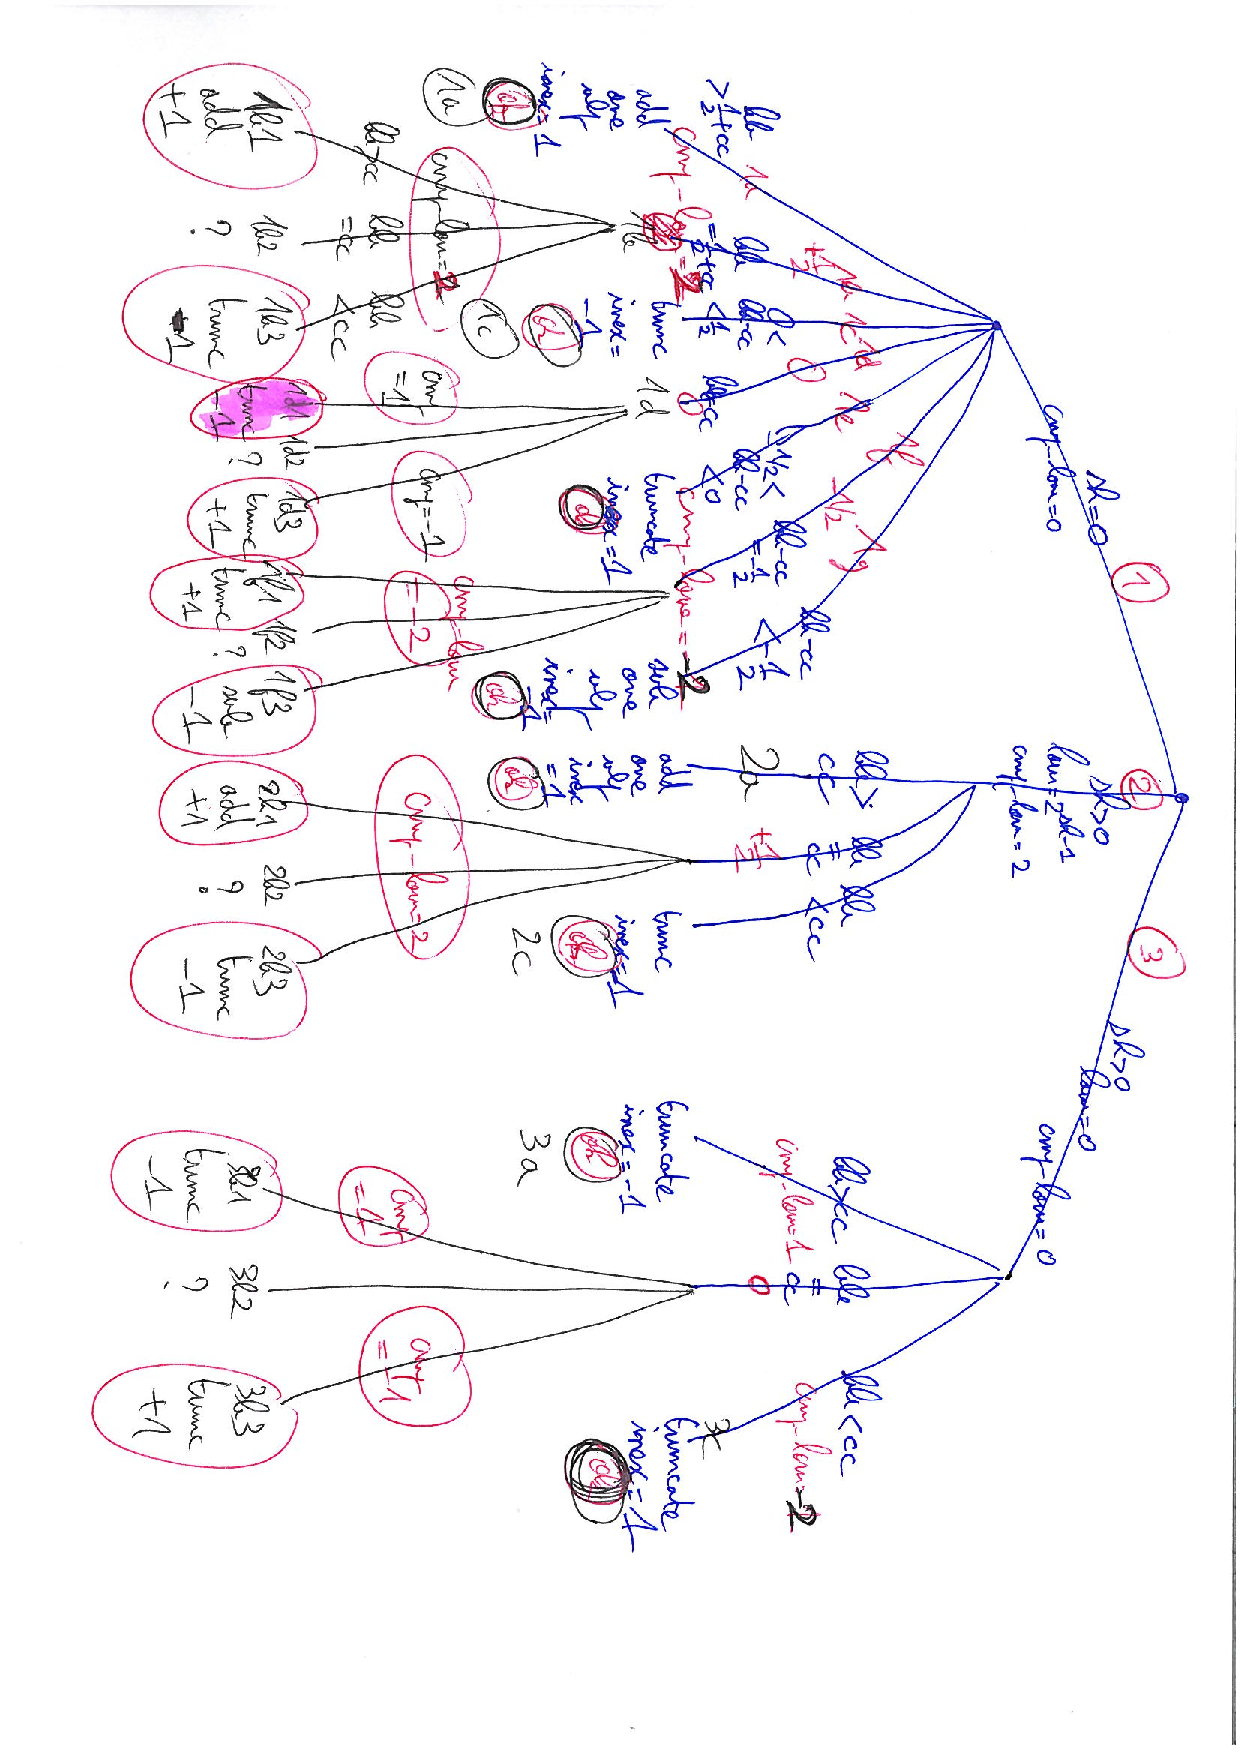
\includegraphics[width=13cm,angle=90]{sub_tree.pdf}}

\subsection{The {\tt mpfr\_mul} function}

{\tt mpfr\_mul} uses two algorithms: if the precision of the operands
is small enough, a plain multiplication using {\tt mpn\_mul} is used
(there is no error, except in the final rounding);
otherwise it uses {\tt mpfr\_mulhigh\_n}.

In this case, it trunks the two operands to $m$ limbs:
$1/2 \leq b < 1$ and $1/2 \leq c < 1$, $b = bh+bl$ and $c = ch+cl$
($B=2^{32} or 2^{64}$).
The error comes from:
\begin {itemize}
\item Truncation: $ \leq bl.ch + bh.cl + bl.cl \leq bl + cl \leq 2 B^{-m}$
\item Mulders: Assuming $\error(Mulders(n)) \leq \error(mulhigh\_basecase(n))$,
\begin{eqnarray*}
\error(mulhigh(n))
  & \leq & (n-1) (B-1)^2 B^{-n-2} + \cdots + 1 (B-1)^2 B^{-2n} \\
  & = & \sum_{i=1}^{n-1}{(n-i) (B-1)^2 B^{-n-1-i}}
    =   (B-1)^2 B^{-n-1} \sum_{i=1}^{n-1}{B^{-i}} \\
  & = & (b-1)^2 B^{-n-1} \frac{B^{1-n}-n+n B-B}{(1-B)^2} \leq n B^{-n}.
\end{eqnarray*}
\end {itemize}
Total error: $\leq (m+2) B^{-m}$.

\subsection{The {\tt mpfr\_div} function}

The goals of the code of the {\tt mpfr\_div} function include the fact
that the complexity should, while preserving correct
rounding, depend on the precision required on the result rather than
on the precision given on the operands.

Let $u$ be the dividend, $v$ the divisor, and $p$ the target precision
for the quotient. We denote by $q$ the real quotient $u/v$, with infinite
precision, and $n \geq p$ the working precision.
The idea --- as in the square root algorithm below --- is to use GMP's
integer division: divide the most $2n$ or $2n-1$ significant bits from $u$ by
the most $n$ significant bits from $v$ will give a good approximation of
the quotient's integer significand.
The main difficulties arise when $u$ and $v$ have a larger precision than
$2n$ and $n$ respectively, since we have to truncate them.
We distinguish two cases: whether the divisor is truncated or not.

\subsubsection{Full divisor.}
This is the easy case. Write $u = u_1 + u_0$ where $u_0$ is the truncated
part, and $v = v_1$. Without loss of generality we can assume that
$\ulp(u_1)=\ulp(v_1)=1$, thus $u_1$ and $v_1$ are integers, and
$0 \leq u_0 < 1$.
Since $v_1$ has $n$ significant bits, we have $2^{n-1} \leq v_1 < 2^n$.
(We normalize $u$ so that the integer quotient gives exactly $n$ bits;
this is easy by comparing the most significant bits of $u$ and $v$,
thus $2^{2n-2} \leq u_1 < 2^{2n}$.)
The integer division of $u_1$ by $v_1$ yields $q_1$ and $r$
such that $u_1 = q_1 v_1 + r$, with $0 \leq r < v_1$, and
$q_1$ having exactly $n$ bits.
In that case we have
\[ q_1 \leq q=\frac{u}{v} < q_1 + 1. \]
Indeed, $q = \frac{u}{v} \geq \frac{u_1}{v_1} = \frac{q_1 v_1 + r}{v_1}$,
and $q \leq \frac{u_1+u_0}{v_1} \leq q_1 + \frac{r + u_0}{v_1} < q_1 + 1$,
since $r + u_0 < r+1 \leq v_1$.

\subsubsection{Truncated divisor.} This is the hard case.
Write $u = u_1 + u_0$, and $v = v_1 + v_0$, where $0 \leq u_0, v_0 < 1$
with the same conventions as above.
We prove in that case that:
\begin{equation} \label{diveq}
q_1-2 < q = \frac{u}{v} < q_1 + 1.
\end{equation}
The upper bound holds as above.
For the lower bound, we have $u - (q_1-2) v >
u_1 - (q_1-2) (v_1+1) \geq q_1 v_1 - (q_1-2) (v_1+1)
= 2 (v_1+1) - q_1 \geq 2^n - q_1 > 0$.
This lower bound is the best possible, since $q_1-1$ would be wrong;
indeed, consider $n=3$, $v_1=4$, $v_0 = 7/8$, $u=24$: this gives $q_1 = 6$,
but $u/v = 64/13 < q_1-1 = 5$.

As a consequence of Eq.~(\ref{diveq}), if the open interval $(q_1-2, q_1+1)$
contains no rounding boundary for the target precision, we can deduce the
correct rounding of $u/v$ just from the value of $q_1$.
In other words, for directed rounding, the two only ``bad cases'' are when
the binary representation of $q_1$ ends with $\underbrace{0000}_{n-p}$
or $\underbrace{0001}_{n-p}$.
We even can decide if rounding is correct, since when $q_1$ ends with $0010$,
the exact value cannot end with $0000$, and similarly
when $q_1$ ends with $1111$.
Hence if $n=p+k$, i.e.\ if we use $k$ extra bits with respect to the target
precision $p$, the failure probability is $2^{1-k}$.

\subsubsection{Avoiding Ziv's strategy.}
In the failure case ($q_1$ ending with $000\ldots 000x$ with directed rounding,
or $100 \ldots 000x$ with rounding to nearest),
we could try again with a larger working precision $p$.
However, we then need to perform a second
division, and we are not sure this new computation will enable us to conclude.
In fact, we can conclude directly. Recall that $u_1 = q_1 v_1 + r$.
Thus $u = q_1 v + (r + u_0 - q_1 v_0)$.
We have to decide which of the following five cases holds:
(a) $q_1 - 2 < q < q_1 - 1$, (b) $q = q_1-1$,
(c) $q_1-1 < q < q_1$, (d) $q=q_1$, (e) $q_1 < q < q_1+1$.
\begin{quote}
$s \leftarrow q_1 v_0$ \\
\textbf{if} $s < r + u_0$ \textbf{then} $q \in (q_1, q_1+1)$ \\
\textbf{elif} $s = r + u_0$ \textbf{then} $q = q_1$ \\
\textbf{else} \\ % u = (q1-1) v + (r + u_0 - s + v)
\q $t \leftarrow s - (r + u_0)$ \\ % u = (q1-1) v + (v - t)
\q \textbf{if} $t < v$ \textbf{then} $q \in (q_1 - 1, q_1)$ \\
\textbf{elif} $t=v$ \textbf{then} $q = q_1-1$ \\
\textbf{else} $q \in (q_1 - 2, q_1-1)$
\end{quote}

\begin{comment}
Let $u = u_n 2^{u_e}$, $v = v_n
2^{v_e}$, where $u_n$ and $v_n$ are in $[1/2, 1[$. Let $q_p$ be the
precision required on $q$. Put
$b_p = \min(v_p, q_p + \varepsilon_p)$,
$a_p = b_p + q_p + \varepsilon_p$, where $\varepsilon_p$ is a small value
to be chosen.

First, a integer division of $u_{hi} = \lfloor
u_n 2^{a_p} \rfloor$ by
$v_{hi} = \lfloor v_n 2^{b_p} \rfloor$
is performed. Write $u_{hi} = \tilde{q} v_{hi} + \tilde{r}$.

If this division is not a full one, to obtain the real value
of the quotient, if $\delta = max(u_p, v_p)$, we have to
divide $u_n 2^{q_p + \varepsilon_p + \delta}$ by
$v_n 2^{\delta}$.

In that case, $2^{q_p + \varepsilon_p + \delta} u_n = \tilde{q}v_n
2^{\delta} + \tilde{r} 2^{\delta - q_p - \varepsilon_p} + u_{lo} -
\tilde{q}v_{lo}$, with obvious notations.

A positive correction on $q$ has to come from the contribution of
$\tilde{r} 2^{\delta - q_p - \varepsilon_p} + u_{lo}$. The
first term is at most $v_{hi} 2^{\delta - q_p - \varepsilon_p}$.
As for $u_{lo}$, we have $u_{lo} < 2^{\delta-q_p-\varepsilon_p}$. Hence,
the sum $u_{lo} + \tilde{r} 2^{\delta - q_p - \varepsilon_p} < 2v$,
and the positive correction is at most 1.

We now have to estimate $\tilde{q}v_{lo}$. It is easily seen that
$\tilde{q} < 2^{q_p + \varepsilon_p + 1}$. As for $v_{lo}$, we have
$v_{lo} < 2^{\delta - q_p - \varepsilon_p}$, so that
$\tilde{q} v_{lo} < 2^{\delta + 1}$, to be compared with $v_n 2^{\delta}$,
so that a negative correction is at most 3. As a consequence, to be able
to decide rounding after the first stage, one should choose
$\varepsilon_p \geq 3$ (to include the round-to-nearest case).
\end{comment}

\subsubsection{Using Mulders' short division}

For larger operands, Mulders' short division might be faster than calling
GMP's integer division. A detailed description of Mulders' short division
for integers can be found in \cite{HaZi11}.
We assume that we want the quotient integer significant on $n-1$ limbs,
and we perform a short division on $n$ limbs.
Let $q$ be the real quotient $u/v$, scaled so that it has exactly $n$ limbs;
let $q_1$ be the integer division we would perform using GMP's integer
division as described above, and let $q_2$ be the approximate quotient
returned by Algorithm \texttt{ShortDiv} or \texttt{FoldDiv} from \cite{HaZi11}.
From the above analysis, we know that $q_1 - 2 < q < q_1 + 1$, the divisor
being truncated or not.
From Theorems~1 and~2 from \cite{HaZi11}, we have
$q_1 - 2n \leq q_2 \leq q_1 + 2n$.
It thus follows:
\[ q_1 - (2n+2) < q < q_2 + (2n+1), \]
and in all cases the difference between $q$ and $q_2$ is less than $2n+2$
ulps (on $n$ limbs).
Since we want to round $q$ on $n-1$ limbs, and usually $2n+2$ is small
compared to the limb value, in most cases we will be able to round correctly.

In the rare cases where we are not able to round correctly, we can either
revert to the above method using integer division, or better use the
approximate quotient $q_2$ to deduce the exact quotient $q_1$ and the
corresponding remainder, which will trade a division for a multiplication.

\subsection{The {\tt mpfr\_sqrt} function}

The \texttt{mpfr\_sqrt} implementation uses the \texttt{mpn\_sqrtrem}
function from GMP's \texttt{mpn} level:
given a positive integer $m$, it computes $s$ and $r$ such that
$m = s^2 + r$ with $s^2 \leq m < (s+1)^2$, or equivalently $0 \leq r \leq 2s$.
In other words, $s$ is the integer square root of $m$, rounded toward zero.

The idea is to multiply the input significand by some power of two,
in order to obtain an integer significand $m$ whose integer square root
$s$ will have exactly $p$ bits, where $p$ is the target precision.
This is easy: $m$ should have either $2p$ or $2p-1$ bits.
For directed rounding, we then know that the result significand will be
either $s$ or $s+1$, depending on the square root remainder $r$ being zero
or not.
\begin{quote}
Algorithm $\texttt{FPSqrt}$. \\
Input: $x = m \cdot 2^e$, a target precision $p$, a rounding mode $\circ$ \\
Output: $y = \circ_p(\sqrt{x})$ \\
If $e$ is odd, $(m', f) \leftarrow (2m, e-1)$, else $(m',f) \leftarrow (m,e)$ \\
Write $m' := m_1 2^{2k} + m_0$, $m_1$ having $2p$ or $2p-1$ bits, $0 \leq m_0 < 2^{2k}$ \\
$(s, r) \leftarrow \texttt{SqrtRem}(m_1)$ \\
If round to zero or down or $r=m_0=0$, return $s \cdot 2^{k+f/2}$ \\
else return $(s+1) \cdot 2^{k+f/2}$.
\end{quote}
In case the input has more than $2p$ or $2p-1$ bits, it needs to be truncated,
but the crucial point is that that truncated part will not overlap with the
remainder $r$ from the integer square root, so the \emph{sticky bit} is
simply zero when both parts are zero.

For rounding to nearest, the simplest way is to ask $p+1$ bits for the
integer square root --- thus $m$ has now $2p+1$ or $2p+2$ bits.
In such a way, we directly get the rounding bit, which is the parity bit
of $s$, and the sticky bit is determined as above.
Otherwise, we have to compare the value of the whole remainder, i.e.\ $r$ plus
the possible truncated input, with $s + 1/4$, since $(s+1/2)^2 =
s^2 + s + 1/4$.
Note that equality can occur --- i.e.\ the ``nearest even rounding rule'' ---
only when the input has at least $2p+1$ bits; in particular it can not
happen in the common case when input and output have the same precision.

\subsection{The inverse square root}

The inverse square root (function \texttt{mpfr\_rec\_sqrt}) is based on
Ziv's strategy and the \texttt{mpfr\_mpn\_rec\_sqrt} function, which given
a precision $p$, and an input $1 \leq a < 4$,
returns an approximation $x$ satisfying 
\[ x - \frac{1}{2} \cdot 2^{-p} \leq a^{-1/2} \leq x + 2^{-p}. \]

The \texttt{mpfr\_mpn\_rec\_sqrt} function is based on Newton's iteration
and the following lemma,
the proof of which can be found in \cite{BrZi06}:
\begin{lemma} \label{lemma3}
Let $A, x > 0$, and $x' = x + \frac{x}{2} (1 - Ax^2)$. Then
\[ 0 \leq A^{-1/2} - x' = \frac{3}{2} \frac{x^3}{\theta^4} (A^{-1/2}-x)^2, \]
for some $\theta \in (x, A^{-1/2})$.
\end{lemma}

We first describe the recursive iteration:
\begin{quote}
Algorithm $\texttt{ApproximateInverseSquareRoot}$. \\
Input: $1 \leq a, A < 4$ and $1/2 \leq x < 1$ with
$x - \frac{1}{2} \cdot 2^{-h} \leq a^{-1/2} \leq x + 2^{-h}$ \\
Output: $X$ with $X - \frac{1}{2} \cdot 2^{-n} \leq A^{-1/2} \leq X + 2^{-n}$,
where $n \leq 2h-3$ \\
\q $r \leftarrow x^2$ \qquad [exact] \\
\q $s \leftarrow A r$ \qquad [exact] \\
\q $t \leftarrow 1-s$ \qquad [rounded at weight $2^{-2h}$ toward $-\infty$]\\
\q $u \leftarrow x t$ \qquad [exact] \\
\q $X \leftarrow x + u/2$ \qquad [rounded at weight $2^{-n}$ to nearest]
\end{quote}

\begin{lemma} \label{lemma_recsqrt}
If $h \geq 11$, $0 \leq A - a < 2^{-h}$, then the output $X$ of algorithm
$\texttt{ApproximateInverseSquareRoot}$ satisfies
\begin{equation} \label{rec_sqrt_eq1}
X - \frac{1}{2} \cdot 2^{-n} \leq A^{-1/2} \leq X + 2^{-n}.
\end{equation}
\end{lemma}
\begin{proof}
Firstly, $a \leq A < a+2^{-h}$ yields
$a^{-1/2} - \frac{1}{2} \cdot 2^{-h} \leq A^{-1/2} \leq a^{-1/2}$,
thus $x - 2^{-h} \leq A^{-1/2} \leq x + 2^{-h}$.

Lemma~\ref{lemma3} implies that the value $x'$ that would return
Algorithm $\texttt{ApproximateInverseSquareRoot}$ if there was no rounding
error satisfies $0 \leq A^{-1/2} - x' = \frac{3}{2} \frac{x^3}{\theta^4} 
(A^{-1/2}-x)^2$. Since $\theta \in (x, A^{-1/2})$, and
$A^{-1/2} \leq x + 2^{-h}$, we have $x \leq \theta + 2^{-h}$,
which yields $\frac{x^3}{\theta^3} \leq (1 + \frac{2^{-h}}{\theta})^3
\leq (1 + 2^{-10})^3 \leq 1.003$ since $\theta \geq 1/2$ and $h \geq 11$.
Thus $0 \leq A^{-1/2} - x' \leq 3.01 \cdot 2^{-2h}$.

Finally the errors while rounding $1-s$ and $x+u/2$ in the algorithm 
yield $\frac{1}{2} \cdot 2^{-n} \leq x' - X \leq \frac{1}{2} \cdot 2^{-n}
+ \frac{1}{2} \cdot 2^{-2h}$, thus the final inequality is:
\[ \frac{1}{2} \cdot 2^{-n} \leq A^{-1/2} - X \leq 
\frac{1}{2} \cdot 2^{-n} + 3.51 \cdot 2^{-2h}. \]
For $2h \geq n+3$, we have $3.51 \cdot 2^{-2h} \leq \frac{1}{2} \cdot 2^{-n}$,
which concludes the proof.
\end{proof}

The initial approximation is obtained using a bipartite table for $h=11$.
More precisely, we split a $13$-bit input $a = a_1 a_0. a_{-1} \ldots a_{-11}$
into three parts of $5$, $4$ and $4$ bits respectively, say $\alpha,
\beta, \gamma$, and we deduce a $11$-bit approximation
$x = 0.x_{-1} x_{-2} \ldots x_{-11}$ of the form
$T_1[\alpha, \beta] + T_2[\alpha,\gamma]$, where both tables have $384$
entries each.
Those tables satisfy:
\[ x + (\frac{1}{4} - \varepsilon) 2^{-11} \leq a^{-1/2} \leq
   x + (\frac{1}{4} + \varepsilon) 2^{-11}, \]
with $\varepsilon \leq 1.061$.
% the worst-case is obtained for a=2289/2048, where
% a^{-1/2} = 1937.1891686292820586, and x = 1938 (shifted by $2^{11}$).
Note that this does not fulfill the initial condition of
Algorithm $\texttt{ApproximateInverseSquareRoot}$, since
we have $x - 0.811 \cdot 2^{-h} \leq a^{-1/2} \leq x + 1.311 \cdot 2^{-h}$,
% 0.811 = 1.061 - 0.25, 1.311 = 1.061 + 0.25
which yields $X - \frac{1}{2} \cdot 2^{-n} \leq A^{-1/2} \leq
              X + 1.21 \cdot 2^{-n}$,
thus the right bound is not a priori fulfilled.
% (3*1.003*1.311^2+0.5)/8+0.5 <= 1.21
However the only problematic case is $n=19$, which gives exactly
$(n+3)/2 = 11$, since for $12 \leq n \leq 18$,
the error terms in $2^{-2h}$ are halved.
An exhaustive search of all possible inputs for $h=11$ and $n=19$ gives
\[ X - \frac{1}{2} \cdot 2^{-n} \leq A^{-1/2} \leq X + 0.998 \cdot 2^{-n},\]
the worst case being $A=1990149, X=269098$ (scaled by $2^{19}$).
Thus as soon as $n \geq 2$, Eq.~(\ref{rec_sqrt_eq1}) is fulfilled.

\medskip

In summary, Algorithm $\texttt{ApproximateInverseSquareRoot}$ provides an
approximation $X$ of $A^{-1/2}$ with an error of at most one ulp.
However if the input $A$ was itself truncated at precision $\geq p$
from an input $A_0$ ---
for example when the output precision $p$ is less than the input precision ---
then we have $|X - A^{-1/2}| \leq \ulp(X)$, and
$|A^{-1/2} - A_0^{-1/2}| \leq \frac{1}{2} |A - A_0| A^{-3/2}
\leq \frac{1}{2} \frac{|A - A_0|}{A} A^{-1/2}
\leq 2^{-p} A^{-1/2} \leq \ulp(X)$, thus
$|X - A_0^{-1/2}| \leq 2 \, \ulp(X)$.

\subsection{The \texttt{mpfr\_remainder} and \texttt{mpfr\_remquo} functions}

The \texttt{mpfr\_remainder} and \texttt{mpfr\_remquo} are useful
functions for argument reduction. Given two floating-point numbers $x$ and
$y$, \texttt{mpfr\_remainder} computes the correct rounding of
$x \cmod y := x - q y$, where
$q = \lfloor x/y \rceil$, with ties rounded to the nearest even integer,
as in the rounding to nearest mode.

Additionally, \texttt{mpfr\_remquo} returns a value congruent to $q$
modulo $2^n$, where $n$ is a small integer (say $n \leq 64$, see the
documentation), and having the same sign as $q$ or being zero.
This can be efficiently implemented by calling \texttt{mpfr\_remainder} on
$x$ and $2^n y$. Indeed, if $x = r' \cmod (2^n y)$, and
$r' = q' y + r$ with $|r| \leq y/2$, then
$q \equiv q' \mod 2^n$. No double-rounding problem can occur, since if
$x/(2^n y) \in {\mathbb Z} + 1/2$,
then $r'=\pm 2^{n-1} y$, thus $q'=\pm 2^{n-1}$ and $r=0$.

Whatever the input $x$ and $y$, it should be noted that if $\ulp(x) \geq
\ulp(y)$, then $x - q y$ is always
exactly representable in the precision of $y$ unless its exponent is smaller
than the minimum exponent. To see this,
let $\ulp(y) = 2^{-k}$;
multiplying $x$ and $y$ by $2^k$ we get $X = 2^k x$ and
$Y = 2^k y$ such that $\ulp(Y)=1$,
and $\ulp(X) \geq \ulp(Y)$, thus both $X$ and $Y$ are integers.
Now perform the division of $X$ by $Y$, with quotient rounded to nearest:
$X = q Y + R$, with $|R| \leq Y/2$. Since $R$ is an integer, it is
necessarily representable with the precision of $Y$, and thus of $y$.
The quotient $q$ of $x/y$ is the same as that of $X/Y$, the remainder
$x - q y$ is $2^{-k} R$.

We assume without loss of generality that $x, y > 0$, and that
$\ulp(y) = 1$, i.e., $y$ is an integer.
\begin{quote}
Algorithm Remainder. \\
Input: $x$, $y$ with $\ulp(y)=1$, a rounding mode $\circ$ \\
Output: $x \cmod y$, rounded according to $\circ$ \\
1. If $\ulp(x) < 1$, decompose $x$ into $x_h + x_l$ with $\ulp(x_h) \geq 1$
   and $0 \leq x_l < 1$. \\
1a. $r \leftarrow \mathrm{Remainder}(x_h, y)$ [exact, $-y/2 \leq r \leq y/2$]\\
1b. if $r < y/2$ or $x_l = 0$ then return $\circ(r + x_l)$ \\
1c. else return $\circ(r + x_l - y) = \circ(x_l - r)$ \\
2. Write $x = m \cdot 2^k$ with $k \geq 0$ \\
3. $z \leftarrow 2^k \bmod y$ [binary exponentiation] \\
4. Return $\circ(mz \cmod y)$.
\end{quote}
Note: at step (1a) the auxiliary variable $r$ has the precision of $y$;
since $x_h$ and $y$ are integers, so is $r$ and the result is exact by the
above reasoning. At step (1c) we have $r=y/2$, thus $r-y$ simplifies to $-r$.

\section{High level functions}

\subsection{The cosine function}

To evaluate $\cos x$ with a target precision of $n$ bits, we use the following
algorithm with working precision $m$, after an additive argument reduction
which reduces $x$ in the interval $[-\pi, \pi]$, using the
\texttt{mpfr\_remainder} function:
\begin{quote}
$k \leftarrow \lfloor \sqrt{n/2} \rfloor$ \\
$r \leftarrow x^2$ rounded up \\ % err <= ulp(r)
$r \leftarrow r/2^{2k}$ \\ % err <= ulp(r)
$s \leftarrow 1, t \leftarrow 1$ \\ % err = 0
{\bf for} $l$ {\bf from} $1$ {\bf while} $\Exp(t) \ge -m$ \\
\q $t \leftarrow t \cdot r$ rounded up \\ % err <= (3*l-1)*ulp(t)
\q $t \leftarrow \frac{t}{(2l-1)(2l)}$ rounded up \\ % err <= 3*l*ulp(t)
\q $s \leftarrow s + (-1)^l t$ rounded down\\ % err <= l/2^m
{\bf do} $k$ times \\
\q $s \leftarrow 2 s^2$ rounded up \\
\q $s \leftarrow s - 1$ \\
return $s$ \\
\end{quote}
The error on $r$ after $r \leftarrow x^2$
is at most $1 \ulp(r)$ and remains $1 \ulp(r)$ after
$r \leftarrow r/2^{2k}$ since that division is just an exponent shift.
By induction, the error on $t$ after step $l$ of the for-loop is at most
$3 l \ulp(t)$.
Hence as long as $3 l \ulp(t)$ remains less than $\le 2^{-m}$
during that loop
(this is possible as soon as $r < 1/\sqrt{2}$)
and the loop goes to $l_0$, the error on $s$ after the for-loop is at most
$2 l_0 2^{-m}$ (for $|r| < 1$, it is easy to check that $s$ will remain
in the interval $[\frac{1}{2}, 1[$, thus $\ulp(s) = 2^{-m}$).
(An additional $2^{-m}$ term represents the truncation error,
but for $l=1$ the value of $t$ is exact, giving $(2 l_0 - 1) + 1 = 2 l_0$.)

Denoting by $\epsilon_i$ the maximal error on $s$ after the $i$th step
in the do-loop, we have $\epsilon_0 = 2 l_0 2^{-m}$ and
$\epsilon_{k+1} \le 4 \epsilon_k + 2^{-m}$,
giving $\epsilon_k \le (2 l_0+1/3) 2^{2k-m}$.

\subsection{The sine function}

The sine function is computed from the cosine, with a working precision of
$m$ bits, after an additive argument reduction in $[-\pi, \pi]$:
\begin{quote}
$c \leftarrow \cos x$ rounded away \\
$t \leftarrow c^2$ rounded away \\
$u \leftarrow 1 - t$ rounded to zero \\
$s \leftarrow {\rm sign}(x) \sqrt{u}$ rounded to zero \\
\end{quote}
This algorithm ensures that the approximation $s$ is between zero and $\sin x$.

Since all variables are in $[-1, 1]$, where $\ulp() \leq 2^{-m}$,
all absolute errors are less than $2^{-m}$.
We denote by $\epsilon_i$ a generic error with $0 \leq \epsilon_i < 2^{-m}$.
We have $c = \cos x + \epsilon_1$;
$t = c^2 + \epsilon_2 = \cos^2 x + 4 \epsilon_3$;
$u = 1 - t - \epsilon_4 = 1 - \cos^2 x - 5 \epsilon_5$;
$|s| = \sqrt{u} - \epsilon_6 =
\sqrt{1 - \cos^2 x - 5 \epsilon_5} - \epsilon_6
\geq \left|\sin x\right| - \frac{5 \epsilon_5}{2 |s|} + \epsilon_6$
(by Rolle's theorem,
$|\sqrt{u} - \sqrt{u'}| \le \frac{1}{2 \sqrt{v}} |u-u'|$ for
$v \in [u, u']$, we apply it here with $u=1 - \cos^2 x - 5 \epsilon_5$,
$u'=1 - \cos^2 x$.)

Therefore, if $2^{e-1} \leq |s| < 2^e$, the absolute error on $s$
is bounded by $2^{-m} (\frac{5}{2} 2^{1-e}+1) \leq 2^{3-m-e}$.

\subsubsection{An asymptotically fast algorithm for sin and cos.}
We extend here the algorithm proposed by Brent for the exponential function
to the simultaneous computation of sin and cos. The idea is the following.
We first reduce the input $x$ to the range $0 < x < 1/2$.
Then we decompose $x$ as follows:
\[ x = \sum_{i=1}^{k} \frac{r_i}{2^{2^i}}, \]
where $r_i$ is an integer, $0 \leq r_i < 2^{2^{i-1}}$.

We define $x_j = \sum_{i=j}^{k} \frac{r_i}{2^{2^i}}$; then $x = x_1$,
and we can write $x_j = \frac{r_j}{2^{2^j}} + x_{j+1}$. Thus with
$S_j := \sin \frac{r_j}{2^{2^j}}$ and $C_j := \cos \frac{r_j}{2^{2^j}}$:
\[ \sin x_j = S_j \cos x_{j+1} + C_j \sin x_{j+1}, \quad
   \cos x_j = C_j \cos x_{j+1} - S_j \sin x_{j+1}. \]
The $2k$ values $S_j$ and $C_j$ can be computed by a binary splitting
algorithm, each one in $O(M(n) \log n)$.
Then each pair $(\sin x_j, \cos x_j)$ can be computed from
$(\sin x_{j+1}, \sin x_{j+1})$ with four multiplies and two additions or
subtractions.

\paragraph{Error analysis.}
We use here Higham's method. We assume that the values of $S_j$
and $C_j$ are approximated up to a multiplicative factor of the form
$(1+u)^3$, where $|u| \leq 2^{-p}$, $p \geq 4$ being the working precision.
We also assume that $\cos x_{j+1}$ and $\sin x_{j+1}$ are
approximated with a factor of the form $(1+u)^{k_j}$.
With rounding to nearest, the values of $S_j \cos x_{j+1}$,
$C_j \sin x_{j+1}$, $C_j \cos x_{j+1}$ and $S_j \sin x_{j+1}$ are thus
approximated with a factor $(1+u)^{k_j+4}$.
The value of $\sin x_j$ is approximated with a factor $(1+u)^{k_j+5}$ since
there all terms are nonnegative.

We now analyze the effect of the cancellation in
$C_j \cos x_{j+1} - S_j \sin x_{j+1}$.
We have $\frac{r_j}{2^{2^j}} < 2^{-2^{j-1}}$, and for simplicity we define
$l := 2^{j-1}$;
thus $0 \leq S_j \leq 2^{-l}$, and $1-2^{-2l-1} \leq C_j \leq 1$.
Similarly we have $x_{j+1} < 2^{-2l}$, thus
$0 \leq \sin x_{j+1} \leq 2^{-2l}$, and $1-2^{-4l-1} \leq \cos x_{j+1} \leq 1$.
The error is multiplied by a maximal ratio of
\[ \frac{C_j \cos x_{j+1} + S_j \sin x_{j+1}}
{C_j \cos x_{j+1} - S_j \sin x_{j+1}} \leq
\frac{1+2^{-l} \cdot 2^{-2l}}{(1-2^{-2l-1})(1-2^{-4l-1})-2^{-l} \cdot 2^{-2l}},
\]
which we can bound by
\[ \frac{1+2^{-3l}}{1-2^{-2l}} \leq \frac{1}{(1-2^{-2l})(1-2^{-3l})}
\leq \frac{1}{1-2^{-2l+1}}. \]
The product of all those factors for $j \geq 1$ is bounded by $3$
(remember $l := 2^{j-1}$).

In summary, the maximal error is of the form $3 [(1+u)^{5k}-1]$, where
$2^{2^{k-1}} < p \leq 2^{2^k}$.
For $p \geq 4$, $5k \cdot 2^{-p}$ is bounded by $5/16$, and
$(1+2^{-p})^{5k} - 1 \leq e^{5k \cdot 2^{-p}} - 1 \leq \frac{6}{5}
\cdot 5k \cdot 2^{-p} = 6k \cdot 2^{-p}$.
Thus the final relative error bound is $18k \cdot 2^{-p}$.
Since $k \leq 6$ for $p \leq 2^{64}$, this gives a uniform relative error
bound of $2^{-p+7}$.

\subsection{The tangent function}

The tangent function is computed from the \texttt{mpfr\_sin\_cos} function,
which computes simultaneously $\sin x$ and $\cos x$
with a working precision of $m$ bits:
\begin{quote}
$s, c \leftarrow \circ(\sin x), \circ(\cos x)$ \quad [to nearest] \\
$t \leftarrow \circ(s/c)$ \quad [to nearest] \\
\end{quote}
We have $s = \sin(x) (1 + \theta_1)$ and $c = \cos(x) (1 + \theta_2)$
with $|\theta_1|, |\theta_2| \leq 2^{-m}$, thus
$t = (\tan x) (1 + \theta)^3$ with $|\theta| \leq 2^{-m}$.
For $m \geq 2$, $|\theta| \leq 1/4$,
$|(1 + \theta)^3 - 1| \leq 4 |\theta|$, thus we can write
$t = (\tan x) (1 + 4 \theta)$, thus
$|t - \tan x| \leq 4 \ulp(t)$.

\subsection{The exponential function}

The {\tt mpfr\_exp} function implements three different algorithms.
For very large precision, it uses a $\O(M(n) \log^2 n)$ algorithm
based on binary splitting (see \cite{Jeandel00}).
This algorithm is used only for precision greater
than for example $10000$ bits on an Athlon.

For smaller precisions, it uses Brent's method;
if $r = (x - n \log 2)/2^k$ where $0 \le r < \log 2$, then
\[ \exp(x) = 2^n \cdot \exp(r)^{2^k} \]
and $\exp(r)$ is computed using the Taylor expansion:
\[ \exp(r) =  1 + r + \frac{r^2}{2!} + \frac{r^3}{3!} + \cdots \]
As $r < 2^{-k}$, if the target precision is $n$ bits, then only
about $l = n/k$ terms of the Taylor expansion are needed.
This method thus requires the evaluation of the Taylor series to
order $n/k$, and $k$ squares to compute $\exp(r)^{2^k}$.
If the Taylor series is evaluated using a naive way, the optimal
value of $k$ is about $n^{1/2}$, giving a complexity of $\O(n^{1/2} M(n))$.
This is what is implemented in {\tt mpfr\_exp2\_aux}.

If we use a baby step/giant step approach, the Taylor series
can be evaluated in $\O(l^{1/2})$ nonscalar multiplications 
--- i.e., with both operands of full $n$-bit size --- as described in
\cite{PaSt73},
thus the evaluation requires $(n/k)^{1/2} + k$ multiplications,
and the optimal $k$ is now about $n^{1/3}$,
giving a total complexity of $\O(n^{1/3} M(n))$.
This is implemented in the function {\tt mpfr\_exp2\_aux2}.
(Note: the algorithm from Paterson and Stockmeyer was rediscovered by Smith,
who named it ``concurrent series'' in \cite{Smith91}.)

\subsection{The logarithm function}

The logarithm function \verb!mpfr_log! is defined using this
approximated formula~\cite{Muller97} based on the arithmetic-geometric
mean (denoted by AG):
$$ \log x \approx \frac{\pi}{\mbox{2~AG(1,4/s)}} - m \log 2  + o(\log x ~2^{-p})$$
with $ s = x \cdot 2^m > 2^{p/2}$.\\


First, the arithmetic-geometric mean $\mbox{AG}(u_0,v_0)$ is computed as in
mathematics with rounding to nearest:
$$ {\tilde u_{n+1}} = {\mathcal N} \left( \sqrt{{\mathcal N}({\tilde u_n}~{\tilde v_n})}~\right) \qquad
 {\tilde v_{n+1}} = \frac{{\mathcal N} ({\tilde u_n} + {\tilde v_n})}{2} $$

We denote by $u_n$ and $v_n$ the exact mathematical values. By
induction, it can be proved that:
$$ u_n~ {\left(1-\frac{\ulp(1)}{2}\right)}^{\frac{3}{2}n+1} \leq {\tilde u_n} \leq  u_n~ {\left(1+\frac{\ulp(1)}{2}\right)}^{\frac{3}{2}n+1}$$
$$ v_n~ {\left(1-\frac{\ulp(1)}{2}\right)}^{\frac{3}{2}n+1} \leq {\tilde v_n} \leq  {\tilde v_n}~ {\left(1+\frac{\ulp(1)}{2}\right)}^{\frac{3}{2}n+1}$$

Then, if $n \ge \lceil \log \left( \frac{v_0 - u_0}{2~u_0}\right) \rceil$,
$$\frac{|{\tilde v_n} - AG(u_0,v_0)|}{v_0} \le n~2^{\frac{3}{2}n+2-p}+8 \cdot 4^{- \frac{2^n~u_0}{v_0 - u_0}}.$$
Therefore the arithmetic-geometric mean can be computed using the
previous error bound and the \verb!mpfr_can_round! function. It
should be noted that the arithmetic-geometric mean of two different
non-zero floating-point numbers is transcendental, therefore there is
no table maker's dilemma here.


From the arithmetic-geometric mean, we deduce the logarithm, naively
bounding the round-off errors. The only point is that the subtraction
may be a cancellation: a maximum of $\log \left(\frac{p \log
  2}{|x-1|}\right)$ bits can be lost.

\subsection{The error function}

Let $n$ be the target precision, and $x$ be the input value.
For $|x| \geq \sqrt{n \log 2}$, we have $|\erf x| = 1$
or $1^{-}$ according to the rounding mode.
Otherwise we use the Taylor expansion.

\subsubsection{Taylor expansion}

\[ \erf z = \frac{2}{\sqrt{\pi}} \sum_{k=0}^{\infty} \frac{(-1)^k}
        {k! (2k+1)} z^{2k+1} \]

\begin{quote}
\verb|erf_0|$(z, n)$, assumes $z^2 \le n/e$ \\
working precision is $m$ \\
$y \leftarrow \circ (z^2)$ [rounded up] \\
$s \leftarrow 1$ \\
$t \leftarrow 1$ \\
{\bf for} $k$ {\bf from} $1$ {\bf do} \\
\q $t \leftarrow \circ (y t)$ [rounded up] \\
\q $t \leftarrow \circ (t/k)$ [rounded up] \\
\q $u \leftarrow \circ (\frac{t}{2k+1})$ [rounded up] \\
\q $s \leftarrow \circ (s + (-1)^k u)$ [nearest] \\
\q {\bf if} $\Exp(u) < \Exp(s) - m$ and $k \geq z^2$
        {\bf then} break \\
$r \leftarrow 2 \circ (z s)$ [rounded up] \\
$p \leftarrow \circ (\pi)$ [rounded down] \\
$p \leftarrow \circ (\sqrt{p})$ [rounded down] \\
$r \leftarrow \circ (r/p)$ [nearest]
\end{quote}

Let $\varepsilon_k$ be the ulp-error on $t$ (denoted $t_k$)
after the loop with index $k$.
According to Lemma~\ref{rel_ulp}, since $t_k$ is computed after $2k$
roundings ($t_0=1$ is exact), we have $\varepsilon_k \leq 4k$.

The error on $u$ at loop $k$ is thus at most
$1+2\varepsilon_k \leq 1+8k$.

Let $\sigma_k$ and $\nu_k$ be the exponent shifts between the new value of
$s$ at step $k$ and respectively the old value of $s$, and $u$.
Writing $s_k$ and $u_k$ for the values of $s$ and $u$ at the end of step $k$,
we have $\sigma_k := \Exp(s_{k-1}) - \Exp(s_k)$
and $\nu_k := \Exp(u_k) - \Exp(s_k)$.
The ulp-error $\tau_k$ on $s_k$ satisfies
$\tau_k \leq \frac{1}{2} + \tau_{k-1} 2^{\sigma_k} + (1+8k) 2^{\nu_k}$.

The halting condition $k \geq z^2$ ensures that $u_j \leq u_{j-1}$ for
$j \geq k$, thus the series $\sum_{j=k}^{\infty} u_j$ is an alternating series,
and the truncated part is bounded by its first term $|u_k| < {\rm ulp}(s_k)$.
So the ulp-error between $s_k$ and $\sum_{k=0}^{\infty} \frac{(-1)^k z^2}{k!
(2k+1)}$ is bounded by $1+\tau_k$.

Now the error after $r \leftarrow 2 \circ (z s)$ is bounded by
$1 + 2 (1+\tau_k) = 2 \tau_k + 3$.
That on $p$ after $p \leftarrow \circ (\pi)$ is $1$ ulp,
and after $p \leftarrow \circ (\sqrt{p})$ we get $2$ ulps
(since $p \leftarrow \circ (\pi)$ was rounded down).

The final error on $r$ is thus at most
$1 + 2 (2 \tau_k + 3) + 4 = 4 \tau_k + 11$
(since $r$ is rounded up and $p$ is rounded down).

\subsubsection{Very large arguments}

Since $\erfc x \leq \frac{1}{\sqrt{\pi} x e^{x^2}}$,
we have for $x^2 \geq n \log 2$ (which implies $x \geq 1$)
that $\erfc x \leq 2^{-n}$, thus
$\erf x = 1$ or $\erf x = 1 - 2^{-n}$ according to the rounding mode.

More precisely, \cite[formul{\ae} 7.1.23 and 7.1.24]{AbSt73} gives:
\[ \sqrt{\pi} x e^{x^2} \erfc x \approx
   1 + \sum_{k=1}^n (-1)^k \frac{1 \times 3 \times \cdots \times (2k-1)}
   {(2x^2)^k}, \]
with the error bounded in absolute value by the next term and of the same sign.

\subsection{The hyperbolic cosine function}

The {\tt mpfr\_cosh} ($\cosh{x}$) function implements the hyperbolic
cosine as :

\[\cosh x = \frac{1}{2} \left( e^{x} + \frac{1}{e^x} \right).\]

The algorithm used for the calculation of the hyperbolic cosine is as follows\footnote{$\circ()$ represent the rounding error and $\error(u)$ the
  error associate with the calculation of $u$}:

\begin{eqnarray}\nonumber
u&\leftarrow&\circ(e^x)\\\label{coshalgo1}
v&\leftarrow&\circ({u}^{-1})\\\label{coshalgo2}
w&\leftarrow&\circ(u+v)\\\label{coshalgo3}
s&\leftarrow&\frac{1}{2} w\\\label{coshalgo4}
\end{eqnarray}

Now, we have to bound the rounding error for each step of this
algorithm.  First, let us consider the parity of hyperbolic cosine
($\cosh(-x)=\cosh(x)$) : the problem is reduced to calculate $\cosh x$
with $x \geq 0$. We can deduce $e^x \geq 1$ and $0 \leq e^{-x} \leq
1$.



\begin{center}
\begin{tabular}{l l l}

\begin{minipage}{2.5cm}


${\textnormal{error}}(u)$


$u \leftarrow \circ(e^x)$\\
$-\infty \;\; (\bullet)$

\end{minipage} &
\begin{minipage}{7.5cm}

\begin{eqnarray}\nonumber
  |u-e^x| &\leq& \ulp(u)\\\nonumber
\end{eqnarray}

\end{minipage} &
\begin{minipage}{6cm}
{\hspace{7cm}}
\end{minipage}\\%\hline
\begin{minipage}{2.5cm}
${\textnormal{error}}(v)$


$v \leftarrow \circ({u}^{-1}) $\\
$+\infty \;\; (\bullet\bullet)$
\end{minipage} &
\begin{minipage}{7.5cm}



\begin{eqnarray}\nonumber
  &&|v-e^{-x}| \\\nonumber
  &       \leq&  |v - u^{-1}| +  |u^{-1}  - e^{-x}|\\\nonumber
  &       \leq& \ulp(v) + \frac{1}{u \cdot e^x} |u-e^{x}|\\\nonumber
  &       \leq& \ulp(v) + \frac{1}{u^2} \ulp(u)\;\;(\star)\\\nonumber
  &       \leq& \ulp(v) + 2 \ulp(\frac{1}{u})\;\;(\star\star)\\\nonumber
  &       \leq& 3 \, \ulp(v)\;\;(\star\star\star)
\end{eqnarray}


\end{minipage} &
\begin{minipage}{6cm}

$(\star)$

With $\frac{1}{e^x} \leq \frac{1}{u}$,\\
for that we must have $u \leq e^x$,\\
it is possible with a rounding of\\
$u$ to $-\infty \;\; (\bullet)$

$(\star\star)$

From inequation \U{R4},
\[   a \cdot \ulp(b) \leq 2 \cdot \ulp(a \cdot b)\]
if $a =\frac{1}{u^2},\;b = u$ then
\[ \frac{1}{u^2} \ulp(u)  \leq 2 \ulp(\frac{1}{u})\]

$(\star\star\star)$

If $\ulp(\frac{1}{u}) \leq ulp(v)$,\\
it is possible with a rounding of \\
$v$ to $+\infty \;\; (\bullet)$\\



\end{minipage}\\%\hline
\begin{minipage}{2.5cm}
${\textnormal{error}}(w)$


$w \leftarrow \circ(u+v) $
\end{minipage} &
\begin{minipage}{7.5cm}



\begin{eqnarray}\nonumber
  &&|w-(e^{x}+e^{-x})| \\\nonumber
  &       \leq&  |w - (u+v)|+|u - e^x|+|v - e^{-x}|\\\nonumber
  &       \leq& \ulp(w) + \ulp(u) + 3\ulp(v)\\\nonumber
  &       \leq& \ulp(w) + 4\ulp(u)\;\;(\star)\\\nonumber
  &       \leq& 5\ulp(w)\;\;(\star\star)\\\nonumber
\end{eqnarray}


\end{minipage} &
\begin{minipage}{6cm}

$(\star)$

With $v \leq 1\leq u$

then $\ulp(v) \leq \ulp(u)$

$(\star\star)$

With $u \leq w$

then $\ulp(u) \leq \ulp(w)$

\end{minipage}\\%\hline
\begin{minipage}{2.5cm}
${\textnormal{error}}(s)$

$s \leftarrow \circ(\frac{w}{2}) $
\end{minipage} &
\begin{minipage}{7.5cm}

\begin{center}


\begin{eqnarray}\nonumber
 {\textnormal{error}}(s) & = &  {\textnormal{error}}(w)\\\nonumber
 & \leq &  5\ulp(s)
\end{eqnarray}



\end{center}

\end{minipage} &
\begin{minipage}{6cm}


\end{minipage}


\end{tabular}
\end{center}

That shows the rounding error on the calculation of $\cosh x$ can be
bound by $5 \;\; \ulp$ on the result. So, to calculate the size of
intermediary variables, we have to add, at least, $\lceil \log_2 5 \rceil=3$ bits the wanted
precision.

\subsection{The inverse hyperbolic cosine function}

The {\tt mpfr\_acosh} function implements the inverse hyperbolic
cosine. For $x < 1$, it returns NaN; for $x=1$, $\acosh x = 0$;
for $x > 1$, the formula $\acosh x = \log ( \sqrt{x^2-1} + x )$
is implemented using the following algorithm:
\begin{quote}
$q \leftarrow \circ(x^2)$ [down] \\
$r \leftarrow \circ(q-1)$ [down] \\
$s \leftarrow \circ(\sqrt{r})$ [nearest] \\
$t \leftarrow \circ(s + x)$ [nearest] \\
$u \leftarrow \circ(\log t)$ [nearest]
\end{quote}

Let us first assume that $r \ne 0$. The error on $q$ is at most $1\,\ulp(q)$,
thus that on $r$ is at most $\ulp(r) + \ulp(q) = (1+E)\,\ulp(r)$ with
$d = \Exp(q) - \Exp(r)$ and $E = 2^d$.
Since $r$ is smaller than $x^2-1$, we can use the simpler formula for the
error on the square root, which gives a bound $(\frac{3}{2} + E)\,\ulp(s)$
for the error on $s$, and $(2 + E)\,\ulp(t)$ for that on $t$. This gives
a final bound of $(\frac{1}{2} + (2 + E) 2^{2-\Exp(u)})\,\ulp(u)$ for the
error on $u$ (\textsection\ref{generic:log}).
We have: $2 + E \leq 2^{1 + \mathrm{max}(1,d)}$. Thus the rounding error
on the calculation of $\acosh x$ can be bounded by
$(\frac{1}{2} + 2^{3 + \mathrm{max}(1,d) - \Exp(u)})\,\ulp(u)$.

If we obtain $r = 0$, which means that $x$ is near from $1$,
we need another algorithm.
One has $x = 1 + z$, with $0 < z < 2^{-p}$, where $p$ is the intermediate
precision (which may be smaller than the precision of $x$). The formula
can be rewritten:
$\acosh x = \log (1 + \sqrt{z(2+z)} + z) = \sqrt{2z} (1 - \varepsilon(z))$
where $0 < \varepsilon(z) < z / 12$.
% > series(log(1+z+sqrt(z*(2+z)))/sqrt(2*z),z=0);
%                             2      3       4       5
%                    z     3 z    5 z    35 z    63 z       (11/2)
%               1 - ---- + ---- - ---- + ----- - ----- + O(z      )
%                    12    160    896    18432   90112
We use the following algorithm:
\begin{quote}
$q \leftarrow \circ(x - 1)$ [down] \\
$r \leftarrow 2q$ \\
$s \leftarrow \circ(\sqrt{r})$ [nearest]
\end{quote}

The error on $q$ is at most $1\,\ulp(q)$, thus the error on $r$ is at most
$1\,\ulp(r)$. Since $r$ is smaller than $2z$, we can use the simpler formula
for the error on the square root, which gives a bound $\frac{3}{2}\,\ulp(s)$
for the error on $s$. The error on $\acosh x$ is bounded by the sum of the
error bound on $\sqrt{2z}$ and $\varepsilon(z) \sqrt{2z} <
\frac{2^{-p}}{12} 2^{1+\Exp(s)} = \frac{1}{6}\,\ulp(s)$.
Thus the rounding error on the calculation of $\acosh x$ can be bounded by
$\left(\frac{3}{2} + \frac{1}{6}\right)\,\ulp(s) < 2\,\ulp(s)$.

\subsection{The hyperbolic sine function}

The {\tt mpfr\_sinh} ($\sinh{x}$) function implements the hyperbolic
sine as :

\[\sinh x = \frac{1}{2} \left( e^{x} - \frac{1}{e^x} \right).\]

The algorithm used for the calculation of the hyperbolic sine is as follows\footnote{$\circ()$ represent the rounding error and $\error(u)$ the
  error associated with the calculation of $u$}:

\begin{eqnarray}\nonumber
u&\leftarrow&\circ(e^x)\\\nonumber
v&\leftarrow&\circ({u}^{-1})\\\nonumber
w&\leftarrow&\circ(u-v)\\\nonumber
s&\leftarrow&\frac{1}{2} w
\end{eqnarray}

Now, we have to bound the rounding error for each step of this
algorithm.  First, let consider the parity of hyperbolic sine
($\sinh(-x)=-\sinh(x)$) : the problem is reduced to calculate $\sinh x$
with $x \geq 0$. We can deduce $e^x \geq 1$ and $0 \leq e^{-x} \leq
1$.



\begin{center}
\begin{tabular}{l l l}

\begin{minipage}{2.5cm}


${\textnormal{error}}(u)$


$u \leftarrow \minf(e^x)$\\
$(\bullet)$

\end{minipage} &
\begin{minipage}{7.5cm}

\begin{eqnarray}\nonumber
  |u-e^x| &\leq& \ulp(u)\\\nonumber
\end{eqnarray}

\end{minipage} &
\begin{minipage}{6cm}
{\hspace{7cm}}
\end{minipage}\\%\hline
\begin{minipage}{2.5cm}
${\textnormal{error}}(v)$


$v \leftarrow \pinf({u}^{-1}) $\\
$(\bullet\bullet)$
\end{minipage} &
\begin{minipage}{7.5cm}



\begin{eqnarray}\nonumber
  &&|v-e^{-x}| \\\nonumber
  &       \leq&  |v - u^{-1}| +  |u^{-1}  - e^{-x}|\\\nonumber
  &       \leq& \ulp(v) + \frac{1}{u \cdot e^x} |u-e^{x}|\\\nonumber
  &       \leq& \ulp(v) + \frac{1}{u^2} \ulp(u)\;\;(\star)\\\nonumber
  &       \leq& \ulp(v) + 2 \ulp(\frac{1}{u})\;\;(\star\star)\\\nonumber
  &       \leq& 3 \, \ulp(v)\;\;(\star\star\star)
\end{eqnarray}


\end{minipage} &
\begin{minipage}{6cm}

$(\star)$

With $\frac{1}{u} \leq \frac{1}{e^x}$,\\
for that we must have $e^x \leq u$,\\
it is possible with $u=\minf(e^x)$ $(\bullet)$

$(\star\star)$

From inequation \U{R4},
\[   a \cdot \ulp(b) \leq 2 \cdot \ulp(a \cdot b)\]
if $a =\frac{1}{u^2},\;b = u$ then
\[ \frac{1}{u^2} \ulp(u)  \leq 2 \ulp(\frac{1}{u})\]

$(\star\star\star)$

If $\ulp(\frac{1}{u}) \leq \ulp(v)$,\\
it is possible with $v=\pinf(u^{-1})$ $(\bullet\bullet)$



\end{minipage}\\%\hline
\begin{minipage}{2.5cm}
${\textnormal{error}}(w)$


$w \leftarrow \circ(u-v) $
\end{minipage} &
\begin{minipage}{7.8cm}



\begin{eqnarray}\nonumber
  &&|w-(e^{x}-e^{-x})| \\\nonumber
  &       \leq&  |w - (u-v)|+|u - e^x|+|-v + e^{-x}|\\\nonumber
  &       \leq& \ulp(w) + \ulp(u) + 3\ulp(v)\\\nonumber
  &       \leq& \ulp(w) + 4\ulp(u)\;\;(\star)\\\nonumber
  &       \leq& (1+ 4 \cdot 2^{\Exp(u)-\Exp(w)}) \ulp(w)\;\;(\star\star)\\\nonumber
\end{eqnarray}


\end{minipage} &
\begin{minipage}{6cm}

$(\star)$

With $v \leq 1\leq u$

then $\ulp(v) \leq \ulp(u)$

$(\star\star)$

see subsection \ref{generic:sous}

\end{minipage}\\%\hline
\begin{minipage}{2.5cm}
${\textnormal{error}}(s)$

$s \leftarrow \circ(\frac{w}{2}) $
\end{minipage} &
\begin{minipage}{7.5cm}

\begin{center}


\begin{eqnarray}\nonumber
 {\textnormal{error}}(s) & = &  {\textnormal{error}}(w)\\\nonumber
 & \leq &  (1+ 4 \cdot 2^{\Exp(u)-\Exp(w)}) \ulp(w)
\end{eqnarray}



\end{center}

\end{minipage} &
\begin{minipage}{6cm}


\end{minipage}


\end{tabular}
\end{center}


That show the rounding error on the calculation of $\sinh x$ can be bound by $(1+ 4 \cdot 2^{\Exp(u)-\Exp(w)}) \ulp(w)$, then the number of bits need to add to the want accuracy to define intermediary variable is :

\[
N_t=\lceil \log_2(1+ 4 \cdot 2^{\Exp(u)-\Exp(w)}) \rceil
\]


\subsection{The inverse hyperbolic sine function}

The {\tt mpfr\_asinh} ($\n{asinh}{x}$) function implements the inverse hyperbolic sine as :

\[\n{asinh} = \log \left( \sqrt{x^2+1} + x \right).\]

The algorithm used for the calculation of the inverse hyperbolic sine is as follows

\begin{eqnarray}\nonumber
s&\leftarrow&\circ(x^2)\\\nonumber
t&\leftarrow&\circ(s+1)\\\nonumber
u&\leftarrow&\circ(\sqrt{t})\\\nonumber
v&\leftarrow&\circ(u+x)\\\nonumber
w&\leftarrow&\circ(\log  v)
\end{eqnarray}


Now, we have to bound the rounding error for each step of this
algorithm.  First, let consider the parity of hyperbolic arc sine
($\n{asinh}(-x)=-\n{asinh}(x)$) : the problem is reduced to calculate $\n{asinh} x$
with $x \geq 0$.

\begin{center}
\begin{tabular}{l l l}

\begin{minipage}{2.5cm}
${\textnormal{error}}(s)$


$s \leftarrow \circ(x^2) $

\end{minipage} &
\begin{minipage}{7.5cm}

\begin{eqnarray}\nonumber
  &&|s-x^2| \\\nonumber
  &       \leq&  \ulp(s)\;\;(\star)\\\nonumber
\end{eqnarray}


\end{minipage} &
\begin{minipage}{6cm}

\end{minipage}\\%\hline
\begin{minipage}{2.5cm}
${\textnormal{error}}(t)$


$t \leftarrow \minf(s+1) $
$(\bullet)$
\end{minipage} &
\begin{minipage}{7.5cm}



\begin{eqnarray}\nonumber
  &&|t-(x^2+1)| \\\nonumber
  &       \leq&  2 \ulp(t) \;\;(\star)\\\nonumber
\end{eqnarray}


\end{minipage} &
\begin{minipage}{6cm}

($\star$)

see subsection \ref{generic:sous}


\end{minipage}\\%\hline
\begin{minipage}{2.5cm}
${\textnormal{error}}(u)$


$u \leftarrow \circ(\sqrt{t}) $


\end{minipage} &
\begin{minipage}{7.5cm}

\begin{eqnarray}\nonumber
  &&|u-\sqrt{x^2+1}| \\\nonumber
  &       \leq& 3 \ulp(u) \;(\star)
\end{eqnarray}


\end{minipage} &
\begin{minipage}{6cm}

($\star$)

see subsection \ref{generic:sqrt}

with ($\bullet$)

\end{minipage}\\%\hline
\begin{minipage}{2.5cm}
${\textnormal{error}}(v)$


$v \leftarrow \circ(u+x) $


\end{minipage} &
\begin{minipage}{7.5cm}

\begin{eqnarray}\nonumber
  &&|v-(\sqrt{x^2+1}+x)| \\\nonumber
  &       \leq& 5 \ulp(v) \;(\star)
\end{eqnarray}


\end{minipage} &
\begin{minipage}{6cm}

($\star$)

see subsection \ref{generic:sous}

\end{minipage}\\%\hline
\begin{minipage}{2.5cm}
${\textnormal{error}}(w)$


$w \leftarrow \circ(\log v) $
\end{minipage} &
\begin{minipage}{7.5cm}

\begin{eqnarray}\nonumber
  &&|w-\log(\sqrt{x^2+1}+x)| \\\nonumber
  &       \leq& (1+5.2^{2-\Exp(w)}) \ulp(w) \;\star
\end{eqnarray}


\end{minipage} &
\begin{minipage}{6cm}

($\star$)

see subsection \ref{generic:log}

\end{minipage}
\end{tabular}
\end{center}

That shows the rounding error on the calculation of $\n{asinh} x$ can
be bound by $ (1+5.2^{2-\Exp(w)})\;\; \ulp$ on the result. So, to
calculate the size of intermediary variables, we have to add, at
least, $\lceil \log_2 (1+5.2^{2-\Exp(w)}) \rceil$ bits the wanted
precision.

\subsection{The hyperbolic tangent function}

The hyperbolic tangent (\texttt{mpfr\_tanh}) is computed from the exponential:
\[ \tanh x = \frac{ e^{2 x} -1 }{ e^{2 x} +1}. \]

The algorithm used is as follows, with working
precision $p$ and rounding to nearest:
\begin{quote}
$u \leftarrow \circ(2 x)$ \\
$v \leftarrow \circ(e^u)$ \\
$w \leftarrow \circ(v+1)$ \\
$r \leftarrow \circ(v-1)$ \\
$s \leftarrow \circ(r/w)$
\end{quote}
Now, we have to bound the rounding error for each step of this
algorithm.  First, thanks to the parity of hyperbolic tangent
--- $\tanh(-x)=-\tanh(x)$ --- we can consider without loss of generality
that $x \geq 0$.

We use Higham's notation, with $\theta_i$ denoting variables such that
$|\theta_i| \leq 2^{-p}$.
Firstly, $u$ is exact. Then $v = e^{2x} (1+\theta_1)$ and
$w = (e^{2x}+1) (1+\theta_2)^2$.
The error on $r$ is bounded by $\frac{1}{2} \ulp(v) + \frac{1}{2} \ulp(r)$.
Assume $\ulp(v) = 2^e \ulp(r)$, with $e \geq 0$;
then the error on $r$ is bounded by $\frac{1}{2} (2^e+1) \ulp(r)$.
We can thus write $r = (e^{2x}-1) (1+\theta_3)^{2^e+1}$,
and then $s = \tanh(x) (1+\theta_4)^{2^e+4}$.

\begin{lemma}
For $|x| \leq 1/2$, and $|y| \leq |x|^{-1/2}$, we have:
\[ |(1+x)^y-1| \leq 2 |y| x. \]
\end{lemma}
\begin{proof}
We have $(1+x)^y = e^{y \log (1+x)}$,
with $|y \log (1+x)| \leq |x|^{-1/2} |\log (1+x)|$.
The function $|x|^{-1/2} \log (1+x)$ is increasing on $[-1/2,1/2]$, and
takes as values $\approx -0.490$ in $x=-1/2$ and $\approx 0.286$ in $x=1/2$,
thus is bounded in absolute value by $1/2$.
This yields $|y \log (1+x)| \leq 1/2$.
Now it is easy to see that for $|t| \leq 1/2$, we have
$|e^t-1| \leq 1.3 |t|$.
Thus $|(1+x)^y-1| \leq 1.3 |y| |\log (1+x)|$.
The result follows from $|\log (1+x)| \leq 1.4 |x|$ for $|x| \leq 1/2$,
and $1.3 \times 1.4 \leq 2$.
\end{proof}

Applying the above lemma for $x=\theta_4$ and $y=2^e+4$,
assuming $2^e+4 \leq 2^{p/2}$,
we get $s = \tanh(x) [1 + 2(2^e+4)\theta_5]$.
Since $2^e+4 \leq 2^{{\rm max}(3,e+1)}$,
the relative error on $s$ is thus bounded by $2^{{\rm max}(4,e+2)-p}$.

\subsection{The inverse hyperbolic tangent function}

The {\tt mpfr\_atanh} ($\n{atanh}{x}$) function implements the inverse
hyperbolic tangent as :

\[\n{atanh} = \frac{1}{2} \log \frac{1+x}{1-x}.\]

The algorithm used for the calculation of the inverse hyperbolic tangent is
as follows:

\begin{eqnarray}\nonumber
s&\leftarrow&\circ(1+x)\\\nonumber
t&\leftarrow&\circ(1-x)\\\nonumber
u&\leftarrow&\circ(\frac{s}{t})\\\nonumber
v&\leftarrow&\circ(\log u)\\\nonumber
w&\leftarrow&\circ(\frac{1}{2} v)
\end{eqnarray}


Now, we have to bound the rounding error for each step of this
algorithm. First, let consider the parity of hyperbolic arc tangent
($\n{atanh}(-x)=-\n{atanh}(x)$) : the problem is reduced to calculate
$\n{atanh} x$ with $x \geq 0$.

\begin{center}
\begin{tabular}{l l l}

\begin{minipage}{2.5cm}
${\textnormal{error}}(s)$


$s \leftarrow \pinf(1+x) $
$(\bullet)$
\end{minipage} &
\begin{minipage}{7.5cm}

\begin{eqnarray}\nonumber
  &&|s-(1+x)| \\\nonumber
  &       \leq&  2 \ulp(s)\;\;(\star)\\\nonumber
\end{eqnarray}


\end{minipage} &
\begin{minipage}{6cm}

see subsection \ref{generic:sous}


\end{minipage}\\%\hline
\begin{minipage}{2.5cm}
${\textnormal{error}}(t)$

$t \leftarrow \minf(1-x) $
$(\bullet\bullet)$
\end{minipage} &
\begin{minipage}{7.5cm}



\begin{eqnarray}\nonumber
  &&|t-(1-x)| \\\nonumber
  &       \leq&  (1+2^{\Exp(x)-\Exp(t)}) \ulp(t) \;\;(\star)\\\nonumber
\end{eqnarray}


\end{minipage} &
\begin{minipage}{6cm}

($\star$)

see subsection \ref{generic:sous}


\end{minipage}\\%\hline
\begin{minipage}{2.5cm}
${\textnormal{error}}(u)$


$u \leftarrow \circ(\frac{s}{t}) $


\end{minipage} &
\begin{minipage}{7.5cm}

\begin{eqnarray}\nonumber
  &&|u-\frac{1+x}{1-x}| \\\nonumber
  &       \leq& (1+ 2 \times 2 + \\\nonumber
  &       \cdots& 2 \times (1+2^{\Exp(x)-\Exp(t)}))\ulp{u} \;(\star)\\\nonumber
  &       \leq& (7+2^{\Exp(x)-\Exp(t)+1})\ulp(u)
\end{eqnarray}


\end{minipage} &
\begin{minipage}{6cm}

($\star$)

see subsection \ref{generic:inv}

with ($\bullet$) and ($\bullet\bullet$)

\end{minipage}\\%\hline
\begin{minipage}{2.5cm}
${\textnormal{error}}(v)$


$v \leftarrow \circ(\log(u)) $


\end{minipage} &
\begin{minipage}{7.5cm}

\begin{eqnarray}\nonumber
  &&|v-(\log{\frac{1+x}{1-x}})| \\\nonumber
  &       \leq& (1+(7+2^{\Exp(x)-\Exp(t)+1}) \\\nonumber
  &       \cdots&  \times 2^{2-\Exp(v)}) \ulp(v)\;(\star)\\\nonumber
  &       \leq& (1+7 \times 2^{2-\Exp(v)} +\\\nonumber
  &       \cdots&  2^{\Exp(x)-\Exp(t)-\Exp(v)+3}) \ulp(v)
\end{eqnarray}


\end{minipage} &
\begin{minipage}{6cm}

($\star$)

see subsection \ref{generic:log}

\end{minipage}\\%\hline
\begin{minipage}{2.5cm}
${\textnormal{error}}(w)$


$w \leftarrow \circ(\frac{1}{2} v) $
\end{minipage} &
\begin{minipage}{7.5cm}

\begin{eqnarray}\nonumber
  &&|w-\frac{1}{2}\log{\frac{1+x}{1-x}}| \\\nonumber
  &       \leq& (1+7 \times 2^{2-\Exp(v)} + \\\nonumber
  &       \cdots&  2^{\Exp(x)-\Exp(t)-\Exp(v)+3}) \ulp(w) \;\star
\end{eqnarray}


\end{minipage} &
\begin{minipage}{6cm}

($\star$) exact


\end{minipage}
\end{tabular}
\end{center}

That shows the rounding error on the calculation of $\n{atanh} x$ can
be bound by $ (1+7 \times 2^{2-\Exp(v)} +
2^{\Exp(x)-\Exp(t)-\Exp(v)+3}) \; \ulp$ on the result. So, to
calculate the size of intermediary variables, we have to add, at
least, $\lceil \log_2 (1+7 \times 2^{2-\Exp(v)} +
2^{\Exp(x)-\Exp(t)-\Exp(v)+3}) \rceil$ bits the wanted precision.

\subsection{The arc-sine function}

\begin{enumerate}
\item We use the formula $\arcsin\,x=\arctan\,\frac{x}{\sqrt{1-x^2}}$
\item When $x$ is near $1$ we will experience uncertainty problems:
\item If $x=a(1+\delta)$ with $\delta$ being the relative error then we will have
\begin{equation*}
1-x=1-a-a\delta=(1-a)[1-\frac{a}{1-a}\delta]
\end{equation*}
So when using the arc tangent programs we need to take into account that decrease in precision.
\end{enumerate}

\subsection{The arc-cosine function} % from Mathieu Dutour

\begin{enumerate}
\item Obviously, we used the formula
\begin{equation*}
\arccos\,x=\frac{\pi}{2}-\arcsin\,x
\end{equation*}
\item The problem of $\arccos$ is that it is $0$ at $1$, so, we have a cancellation problem to treat at $1$.
\item (Suppose $x\geq 0$, this is where the problem happens) The derivative of $\arccos$ is $\frac{-1}{\sqrt{1-x^2}}$ and we will have
\begin{equation*}
\frac{1}{2\sqrt{1-x}}  \leq   |\frac{-1}{\sqrt{1-x^2}}|=\frac{1}{\sqrt{(1-x)(1+x)}}  \leq  \frac{1}{\sqrt{1-x}}
\end{equation*}
So, integrating the above inequality on $[x,1]$ we get
\begin{equation*}
\sqrt{1-x}\leq \arccos\,x\leq 2\sqrt{1-x}
\end{equation*}
\item The important part is the lower bound that we get which tell us a upper bound on the cancellation that will occur:\\
The terms that are canceled are $\pi/2$ and $\arcsin\,x$, their order is $2$. The number of canceled terms is so
\begin{verbatim}
1-1/2*MPFR_EXP(1-x)
\end{verbatim}
\end{enumerate}

\subsection{The arc-tangent function} % from Mathieu Dutour

The arc-tangent function admits the following argument reduction:
\[ \arctan x = 2 \arctan \frac{x}{1+\sqrt{1+x^2}}
             = 2 \arctan \frac{\sqrt{1+x^2}-1}{x}. \]
If applied once, it reduces the argument to $|x| < 1$, then each successive
application reduces $x$ by a factor of at least $2$.

Assume $|x| \leq 1$. 
We approximate $\frac{\sqrt{1+x^2}-1}{x}$ using the following algorithm:
\begin{quote}
$s \leftarrow \circ(x^2)$ [nearest] \\
$t \leftarrow \circ(1+s)$ [nearest] \\
$u \leftarrow \circ(\sqrt{t})$ [nearest] \\
$v \leftarrow \circ(u-1))$ [nearest] \\
$w \leftarrow \circ(\frac{v}{x})$ [nearest]
\end{quote}
Assuming all computations are done with precision $p$, and denoting
$\theta_i$ a value such that $|\theta_i| \leq 2^{-p}$, we have
$s = x^2 (1+\theta_1)$, $t = (1+s) (1+\theta_2) =
(1 + x^2 (1+\theta_1)) (1+\theta_2) = (1+x^2) (1+\theta_3)^2$,
$u = \sqrt{t} (1+\theta_4) = \sqrt{1+x^2} (1+\theta_3) (1 + \theta_4)
= \sqrt{1+x^2} (1 + \theta_5)^2$.
Now let us write $u - 1 = (\sqrt{1+x^2}-1) (1 + \lambda)$; we have
\[ \lambda = \frac{\sqrt{1+x^2}}{\sqrt{1+x^2}-1} (2 \theta_5 + \theta_5^2). \]
For $|x| \leq 1$, we have $2/x^2 \leq \frac{\sqrt{1+x^2}}{\sqrt{1+x^2}-1}
\leq (2+\sqrt{2})/x^2$, and for $p \geq 5$ the expression
$(2+\sqrt{2}) (2 \theta_5 + \theta_5^2)$ is bounded by $7 \theta_5$, thus we
can write $u - 1 = (\sqrt{1+x^2}-1) (1 + 7 \theta_5/x)$.
It follows $v = (u-1) (1 + \theta_6)$ and
$w = \frac{\sqrt{1+x^2}-1}{x} (1 + 7 \theta_5/x) (1 + \theta_7)^2$.
Still for $|x| \leq 1$ and $p \geq 5$, the product
$(1 + 7 \theta_5/x) (1 + \theta_7)^2$ can be written
$(1 + 10 \theta_8/x)$, thus we have
$w = \frac{\sqrt{1+x^2}-1}{x} (1 + 10 \theta_8/x)$, and the relative
error on $w$ is bounded by $10/x \cdot 2^{-p}$.

Now if we want to apply several times this argument reduction, we need to
analyze the error when $x$ is not exact, but say $x = \bar{x} (1 + \varepsilon
\theta)$, with $\varepsilon \geq 0$ a parameter, and $|\theta| \leq 2^{-p}$.
The above analysis remains valid with $x$ replaced by $\bar{x} (1 + \varepsilon
\theta)$, thus we get $w = f(x) (1 + 10 \theta_8/x)$,
with $f(x) = \frac{\sqrt{1+x^2}-1}{x}$, and $x = \bar{x} (1 + \varepsilon
\theta)$. The derivative of $f$ is bounded by $1/2$ for $|x| \leq 1$, thus
$|f(x) - f(\bar{x})| \leq \frac{1}{2} \varepsilon \bar{x}$. Thus we have
\[ w = \frac{\sqrt{1+\bar{x}^2}-1}{\bar{x}} (1 + \frac{\varepsilon\theta_9}{2})
(1 + 10 \theta_8/x). \]
Assuming $\varepsilon \leq 21/x$, we have
$w = \frac{\sqrt{1+\bar{x}^2}-1}{\bar{x}} (1 + \frac{21}{2} \theta_{10}/x)
(1 + 10 \theta_8/x) = \frac{\sqrt{1+\bar{x}^2}-1}{\bar{x}}
(1 + 21 \theta_{11}/x)$, as long as $|x| \geq 210 \cdot 2^{-p}$.
Since initially $\varepsilon=0$, this proves by induction that
$\varepsilon \leq 21/x$, and the relative error on $w$ after several
argument reductions is bounded by $21/x \cdot 2^{-p}$, where $x$ is the last
reduced argument.
Since the arc-tangent function has a derivative less than $1$,
the corresponding absolute error bound for
$\arctan w$ is also $21/x \cdot 2^{-p}$.
Since $\arctan\frac{\sqrt{1+x^2}-1}{x} \geq 5x/16$ for $0 \leq x \leq 1$,
the relative error bound on $\arctan\frac{\sqrt{1+x^2}-1}{x}$ is
$2^{7-p}/x^2 \leq 2^{9-2\Exp(x)-p}$.

\subsubsection{Binary splitting}
\noindent The Taylor series for $\arctan$ is suitable for analysis using Binary splitting.
\par This method is detailed for example in ``Pi and The AGM'' p 334. It is efficient for rational numbers and is non efficient for non rational numbers.
\par The efficiency of this method is then quite limited. One can then wonder how to use it for non rational numbers.
\par Using the formulas
\begin{equation*}
\arctan\,(-x)=-\arctan\,x\;\;\mbox{and}\;\;\arctan\,x+\arctan\,\frac{1}{x}=\frac{\pi}{2}{\rm sign}(x)
\end{equation*}
we can restrict ourselves to $0\leq x\leq 1$.
\par Writing
\begin{equation*}
x=\sum_{i=1}^{\infty} \frac{u_i}{2^i}\;\;\mbox{with}\;\;u_i\in\{0,1\}
\end{equation*}
or
\begin{equation*}
x=\sum_{i=1}^{\infty} \frac{u_i}{2^{2^i}}\;\;\mbox{with}\;\;u_i\in\{0,1,\dots,2^{2^{i-1}}\}\mbox{~if~}i>1\mbox{~and~}u_1\in \{0,1\}
\end{equation*}
we can compute $\cos$,  $\sin$ or $\exp$ using the formulas
\begin{equation*}
\begin{array}{c}
\cos\,(a+b)=\cos\,a\cos\,b-\sin\,a\sin\,b\\
\sin\,(a+b)=\sin\,a\cos\,b+\cos\,a\sin\,b\\
\exp(a+b)=(\exp\,a)(\exp\,b)
\end{array}
\end{equation*}
Unfortunately for $\arctan$ there is no similar formulas. The only formula known is
\begin{equation*}
\arctan\,x+\arctan\,y=\arctan\,\frac{x+y}{1-xy}+k\pi\;\;\mbox{with}\;\;k\in\Z
\end{equation*}
we will use
\begin{equation*}
\arctan\,x=\arctan\,y+\arctan\,\frac{x-y}{1+xy}
\end{equation*}
with $x,y>0$ and $y<x$.
\par Summarizing we have the following facts:
\begin{enumerate}
\item We can compute efficiently $\arctan\,\frac{u}{2^{2^k}}$ with $k\geq 0$ and $u\in\{0,1,\dots,2^{2^{k-1}}\}$
\item We have a sort of addition formula for $\arctan$, the term $k\pi$ being zero.
\end{enumerate}
So I propose the following algorithm for $x$ given in $[0,1]$.
\begin{enumerate}
\item Write $v_k=2^{2^k}$
\item Define
\begin{equation*}
s_{k+1}=\frac{s_k-A_k}{1+s_kA_k}\;\;\mbox{and}\;\;s_0=x
\end{equation*}
\item $A_k$ is chosen such that
\begin{equation*}
0\leq s_k-A_k<\frac{1}{v_k}
\end{equation*}
and $A_k$ is of the form $\frac{u_k}{v_k}$ with $u_k\in\N$.
\item We have the formula
\begin{equation*}
\begin{array}{rcl}
\arctan\,x
&=&\arctan\,A_0+\arctan\,s_1\\
&=&\arctan\,A_0+\arctan\,A_1+\arctan\,s_2\\
&=&\arctan\,A_0+\dots+\arctan\,A_N+\arctan\,s_{N+1}
\end{array}
\end{equation*}
the number $s_N$ is decreasing toward $0$ and we then have
\begin{equation*}
\begin{array}{rcl}
\arctan\,x&=&\sum_{i=0}^{i=\infty}\arctan\,A_i
\end{array}
\end{equation*}

\end{enumerate}
The drawbacks of this algorithm are:
\begin{enumerate}
\item Complexity of the process is high, higher than the AGM. Nevertheless there is some hope that this can be more efficient than AGM in the domain where the number of bits is high but not too large.
\item There is the need for division which is computationally expensive.
\item We may have to compute $\arctan\,(1/2)$.
\end{enumerate}

\subsubsection{Estimate of absolute error}
\noindent By that analysis we mean that $a$ and $b$ have absolute error $D$ if $|a-b|\leq D$.\\
I give a remind of the algorithm:
\begin{enumerate}
\item Write $v_k=2^{2^k}$
\item Define
\begin{equation*}
s_{k+1}=\frac{s_k-A_k}{1+s_kA_k}\;\;\mbox{and}\;\;s_0=x
\end{equation*}
\item $A_k$ is chosen such that
\begin{equation*}
0\leq s_k-A_k<\frac{1}{v_k}
\end{equation*}
and $A_k$ is of the form $\frac{u_k}{v_k}$ with $u_k\in\N$.
\item We have the formula
\begin{equation*}
\begin{array}{rcl}
\arctan\,x
&=&\arctan\,A_0+\arctan\,s_1\\
&=&\arctan\,A_0+\arctan\,A_1+\arctan\,s_2\\
&=&\arctan\,A_0+\dots+\arctan\,A_N+\arctan\,s_{N+1}
\end{array}
\end{equation*}
the number $s_N$ is very rapidly decreasing toward $0$ and we then have
\[\arctan\,x = \sum_{i=0}^{i=\infty}\arctan\,A_i\]
\item The approximate arc tangent is then
\[\sum_{i=0}^{i=N_0}\arctan_{m_i}\,A_i\]
with $\arctan_{m_i}$ being the sum of the first $2^{m_i}$ terms of the
Taylor series for $\arctan$.
\end{enumerate}
We need to estimate all the quantities involved in the computation.
\begin{enumerate}
\item We have the upper bound
\begin{equation*}
0\leq s_{k+1}=\frac{s_k-A_k}{1+s_kA_k}\leq s_k-A_k\leq \frac{1}{v_k}
\end{equation*}
\item The remainder of the series giving $\arctan\,x$ is
\begin{eqnarray*}
\sum_{i=N_0+1}^{\infty}\arctan\,A_i
&\leq &\sum_{i=N_0+1}^{\infty}A_i\\
&\leq &\sum_{i=N_0+1}^{\infty}s_i\\
&\leq &\sum_{i=N_0+1}^{\infty}\frac{1}{v_{i-1}}\\
&\leq &\sum_{i=N_0}^{\infty}\frac{1}{v_{i}}\\
&\leq &\sum_{i=N_0}^{\infty}\frac{1}{2^{2^i}}=\frac{c_{N_0}}{2^{2^{N_0}}}
\end{eqnarray*}
With $c_{N_0}\leq 1.64$. If $N_0\geq 1$ then $c_{N_0}\leq 1.27$. If $N_0\geq 2$ then $c_{N_0}\leq 1.07$.\\
It remains to determine the right $N_0$.
\item The partial sum of the Taylor series for $\arctan$ have derivative bounded by $1$ and consequently don't increase error.
\item The error created by using the partial sum of the Taylor series of $\arctan$ is bounded by
\begin{equation*}
\frac{(A_i)^{2\times 2^{m_i}+1}}{2*2^{m_i}+1}
\end{equation*}
and is thus bounded by
\begin{eqnarray*}
\frac{1}{2 \times 2^{m_i}+1} [\frac{1}{2^{2^{i-1}}}]^{2\times 2^{m_i}+1}
&=&\frac{1}{2 \times 2^{m_i}+1} [2^{-2^{i-1}}]^{2\times 2^{m_i}+1}\\
&\leq &\frac{1}{2 \times 2^{m_i}+1} [2^{-2^{i-1}}]^{2\times 2^{m_i}}\\
&\leq &\frac{1}{2 \times 2^{m_i}+1} 2^{-2^{i+m_i}}
\end{eqnarray*}
The calculation of $\frac{\arctan\,A_i}{A_i}$ is done by using integer arithmetic and returning a fraction that is converted to mpfr type so there is no error. But to compute $\arctan\,A_i=A_i[\frac{\arctan\,A_i}{A_i}]$ we need to use real arithmetic so there is $1 ulp$ error.\\
In total this is $(N_0) ulp$.
\item Addition give $1 ulp$ There are $(N_0-1)$ addition so we need to take $(N_0 -1) ulp$.
\item The division yields errors:
\begin{enumerate}
\item Having errors in the computation of $A_i$ is of no consequences: It changes the quantity being arc-tangented and that's all. Errors concerning the computation of $s_{N+1}$ in contrary adds to the error.
\item The subtract operation $s_i-A_i$ has the effect of subtracting very near numbers. But $A_i$ has exactly the same first $1$ and $0$ than $s_i$ so we can expect this operation to be nondestructive.
\item Extrapolating from the previous result we can expect that the error of the quantity $\frac{s_i-A_i}{1+s_iA_i}$ is $err(s_i)+1 ulp$
\end{enumerate}
\item The total sum of errors is then (if no errors are done in the counting of errors)
\begin{eqnarray*}
Err(\arctan)
&=&\sum_{i=0}^{i=N_0}\frac{1}{2*2^{m_i}+1}2^{-2^{i+m_i}}+\frac{c_{N_0}}{2^{2^{N_0}}}+(N_0-1)2^{-Prec}\\
&+&(N_0 -1)2^{-Prec}+(N_0)2^{-Prec}\;\;\;[m_i=N_0-i]\\
&=&\sum_{i=0}^{i=N_0}\frac{1}{2*2^{N_0-i}+1}2^{-2^{N_0}}+\frac{c_{N_0}}{2^{2^{N_0}}}+(3*N_0-2)2^{-Prec}\\
&=&\sum_{i=0}^{i=N_0}\frac{1}{2*2^{i}+1}2^{-2^{N_0}}+\frac{c_{N_0}}{2^{2^{N_0}}}+(3*N_0-2)2^{-Prec}\\
&\leq &\{\sum_{i=0}^{i=\infty}\frac{1}{2*2^{i}+1}\}2^{-2^{N_0}}+\frac{c_{N_0}}{2^{2^{N_0}}}+(3*N_0-2)2^{-Prec}\\
&\leq&\{0.77\}2^{-2^{N_0}}+\frac{1.63}{2^{2^{N_0}}}+(3*N_0-2)2^{-Prec}\\
&=&\frac{2.4}{2^{2^{N_0}}}+(3*N_0-2)2^{-Prec}
\end{eqnarray*}
This is what we wish thus $Err(\arctan)< 2^{-prec\_arctan}$ with $prec\_arctan$
is the requested precision on the arc-tangent.
We thus want:
\[\frac{2.4}{2^{2^{N_0}}}\leq 2^{-prec\_arctan-1}\]
and
\[(3 \times N_0-2)2^{-Prec}\leq 2^{-prec\_arctan-1}\]
i.e.
\[N_0\geq \frac{\ln\,(prec\_arctan+1+\frac{\ln\,2.4}{\ln\,2})}{\ln\,2}\]
that we approach by (since the logarithm is expensive):
\begin{equation*}
N_0=ceil(\log(prec\_arctan+2.47)*1.45)
\end{equation*}
and we finally have:
\begin{equation*}
Prec=prec\_arctan+\{1+ceil(\frac{\ln\,(3N_0-2)}{\ln\,2})\}
\end{equation*}
\end{enumerate}

\subsubsection{Estimate of the relative error}
\noindent we say that $a$ and $b$ have relative error $\delta$ if
\begin{equation*}
a=b(1+\Delta)\mbox{~with~}|\Delta|\leq \delta
\end{equation*}
This is the error definition used in mpfr. So we need to redo everything in order to have a consistent analysis.
\begin{enumerate}
\item We can use all previous estimates:
\begin{enumerate}
\item Remainder estimate:
\begin{equation*}
\sum_{i=N_0+1}^{\infty}\arctan\,A_i\leq \frac{c_{N_0}}{2^{2^{N_0}}}
\end{equation*}
so the relative error will be $\frac{1}{\arctan\,x}\frac{c_{N_0}}{2^{2^{N_0}}}$.
\item The relative error created by using a partial sum of Taylor series is
bounded by $\frac{1}{\arctan\,A_i}\frac{1}{2 \times 2^{m_i}+1} 2^{-2^{i+m_i}}$.
\item The multiplication $\arctan\,A_i=A_i[\frac{\arctan\,A_i}{A_i}]$ takes
1 ulp of relative error.
\item Doing the subtraction $s_i-A_i$ is a gradual underflow operation:
it decreases the precision of $s_i-A_i$.
\item The multiplication $a_iA_i$ creates $1$ ulp of error. This is not
much and this relative error is further reduced by adding $1$.
\end{enumerate}
\end{enumerate}



\begin{enumerate}
\item We have
\begin{equation*}
\begin{array}{rcl}
\arctan\,b(1+\Delta)
&=&\arctan(b+b\Delta)\\
&\sim&\arctan\,b+\frac{1}{1+b^2}(b\Delta)\\
&=&[\arctan\,b][1+\{\frac{b}{(1+b^2)\arctan\,b}\}\Delta]
\end{array}
\end{equation*}
A rapid analysis gives $0\leq \frac{b}{(1+b^2)\arctan\,b}\leq 1$ and then we can say that the function $\arctan$ does not increase the relative error.
\item So we have two possible solutions:
\begin{enumerate}
\item Do a relative analysis of our algorithm.
\item Use the previous analysis since the absolute error $D$ is obviously equal to $|b|\delta$ ($\delta$ being the relative error)
\end{enumerate}
it is not hard to see that second solution is certainly better: The formulas are additive. Our analysis will work without problems.
\item It then suffices to replace in the previous section $2^{-prec\_arctan}$ by $2^{-prec\_arctan}\arctan\,x$.
\item If $|x|\leq 1$ then $|\arctan\,x|$ is bounded below by $|x|\frac{4}{\pi}\sim |x|1.27$. So it suffices to have an absolute error bounded above by
\begin{equation*}
2^{-prec\_arctan}\,|x|1.27
\end{equation*}
In this case we will add $2-MPFR\_EXP(x)$ to $prec\_arctan$
\item If $|x|\geq 1$ then $\arctan\,x$ is bounded below by $\frac{\pi}{4}$. So it suffices to have an absolute error bounded above by
\begin{equation*}
2^{-prec\_arctan}\, 1.27
\end{equation*}
we will add $1$ to $prec\_arctan$.\\
In this case we need to take into account the error caused by the subtraction:
\begin{equation*}
\arctan\,x=\pm\frac{\pi}{2}-\arctan\,\frac{1}{x}
\end{equation*}


\end{enumerate}




\subsubsection{Implementation defaults}
\begin{enumerate}
\item The computation is quite slow, this should be improved.
\item The precision should be decreased after the operation $s_i-A_i$. And several other improvement should be done.
\end{enumerate}

\subsection{The Euclidean distance function}

The \texttt{mpfr\_hypot} function implements the Euclidean distance function:
\[
\textnormal{hypot} (x,y) = \sqrt{x^2+y^2}.
\]
If one of the variables is zero, then hypot is computed using the absolute
value of the other variable.  Assume that $0 < y \leq x$. Using the first
degree Taylor polynomial, we have:
\[
0 < \sqrt{x^2+y^2}-x < \frac{y^2}{2x}.
\]

Let $p_x$, $p_y$ be the precisions of the input variables $x$ and $y$
respectively, $p_z$ the output precision and $z=\circ_{p_z}(\sqrt{x^2+y^2})$
the expected result.  Let us assume, as it is the case in MPFR, that
the minimal and maximal acceptable exponents (respectively $e_{min}$
and $e_{max}$) satisfy $2 < e_{max}$ and $e_{max} = -e_{min}$.

When rounding to nearest, if $p_x \leq p_z$ and $\frac{p_z+1}{2} < \Exp(x) -
\Exp(y)$, we have $\frac{y^2}{2x} < \frac{1}{2}\ulp_{p_z}(x)$; if $p_z <
p_x$, the condition $\frac{p_x+1}{2} < \Exp(x) - \Exp(y)$ ensures that
$\frac{y^2}{2x} < \frac{1}{2} \ulp_{p_x}(x)$.  In both cases, these
inequalities show that $z=\N_{p_z}(x)$, except that tie case is rounded
toward plus infinity since hypot($x$,$y$) is strictly greater than $x$.

With the other rounding modes, the conditions $p_z/2 < \Exp(x) - \Exp(y)$
if $p_x \leq p_z$, and $p_x/2 < \Exp(x) - \Exp(y)$ if $p_z < p_x$ mean in
a similar way that $z=\circ_{p_z}(x)$, except that we need to add one ulp
to the result when rounding toward plus infinity and $x$ is exactly
representable with $p_z$ bits of precision.

When none of the above conditions are satisfied, we use the following
algorithm, whose precision is guaranteed when
$\Exp(x) - \Exp(y) \leq e_{max} - 1$:

\begin{quote}
  Algorithm {\tt hypot\_1}\\
  Input: $x$ and $y$ with $|y| \leq |x|$,
  $p$ the working precision with $p \geq p_z$.\\
  Output: $\sqrt{x^2+y^2}$ with $\left\{
  \begin{array}{l}
    p-4 \textnormal{ bits of precision if } p < \max(p_x, p_y),\\
    p-2 \textnormal{ bits of precision if } p \geq \max(p_x, p_y).
  \end{array}\right.$\\
  $s \leftarrow \lfloor (e_{max}-1)/2 \rfloor - \Exp(x)$\\
  $x_s \leftarrow \Z(x\times 2^s)$\\
  $y_s \leftarrow \Z(y\times 2^s)$\\
  $u \leftarrow \Z(x_s^2)$\\
  $v \leftarrow \Z(y_s^2)$\\
  $w \leftarrow \Z(u+v)$\\
  $t \leftarrow \Z(\sqrt{w})$\\
  $z \leftarrow \Z(t/2^s)$
\end{quote}

In order to avoid undue overflow during computation, we shift inputs'
exponents by $s = \lfloor\frac{e_{max}-1}{2}\rfloor - \Exp(x)$ before
computing squares and shift back the output's exponent by $-s$ using the fact
that $\sqrt{(x.2^s)^2+(y.2^s)^2}/2^s = \sqrt{x^2+y^2}$. We show below that
overflow cannot occur, and underflow cannot occur either when
$\Exp(x) - \Exp(y) \leq e_{max} - 1$.

We check first that the exponent shift does not cause overflow and, in the
same time, that the squares of the shifted inputs never overflow.
For $x$, we have $\Exp(x) + s = \lfloor (e_{max}-1)/2 \rfloor$, so
$\Exp(x_s^2) \leq e_{max} - 1$ and neither $x_s$ nor $x_s^2$ overflows.
Therefore we have: $\Z(x_s^2) \leq x_s^2 < 2^{e_{max} - 1}$.
For $y$, note that we have $y_s \leq x_s$ because $y \leq x$, thus $y_s$
and $y_s^2$ do not overflow.

Secondly, let us see that the exponent shift does not cause underflow. For
$x$, we know that $0 \leq \Exp(x) + s$, thus neither $x_s$ nor $x_s^2$
underflows. For $y$, the condition $\Exp(x) - \Exp(y) \leq e_{max} - 1$
implies that $\lfloor(e_{max}-1)/2\rfloor - s - \Exp(y) \leq e_{max} - 1$,
and since $e_{max}/2-1 \leq \lfloor(e_{max}-1)/2\rfloor$, we deduce
$e_{min}/2 = -e_{max}/2 \leq \Exp(y) + s$, which shows that $y_s$ and
its square do not underflow (even when taking the rounding into account
since the scaling is exact).

Thirdly, the addition does not overflow because $u + v < 2 x_s^2$ and it was
shown above that $\Z(x_s^2) < 2^{e_{max} - 1}$. It cannot underflow because
both operands are positive.

Fourthly, as $x_s < t$, the square root does not underflow. Due to the
exponent shift, we have $1 \leq x_s$, then $w$ is greater than 1 and thus
greater than its square root $t$, so the square root does overflow.

Finally, let us show that the back shift raises neither underflow nor overflow
unless the exact result is greater than or equal to $2^{e_{max}}$. Because no
underflow has occurred so far $\Exp(x) \leq \Exp(t) - s$ which shows that it
does not underflow. And all roundings being toward zero, we have $z \leq
\sqrt{x^2 + y^2}$, so if $2^{e_{max}} \leq z$, then the exact value is also
greater than or equal to $2^{e_{max}}$.

Let us analyse now the error of the algorithm hypot\_1:\\
\begin{tabular}{l p{2em} l c r | r}
  & & & & $p < \min(p_x, p_y)$ & $\max(p_x, p_y) \leq p$\\
  $x_s \leftarrow \Z(x\times 2^s)$ & & $\error(x_s)$ & $\leq$ &
  1 $\ulp(x_s)$ &
  exact\\
  $y_s \leftarrow \Z(y\times 2^s)$ & & $\error(y_s)$ & $\leq$ &
  1 $\ulp(y_s)$ &
  exact\\
  $u \leftarrow \Z(x_s^2)$ & & $\error(u)$ & $\leq$ &
  6 $\ulp(u)$ &
  1 $\ulp(u)$\\
  $v \leftarrow \Z(y_s^2)$ & & $\error(v)$ & $\leq$ &
  6 $\ulp(v)$ &
  1 $\ulp(v)$\\
  $w \leftarrow \Z(u+v)$ & & $\error(w)$ & $\leq$ &
  13 $\ulp(w)$ &
  3 $\ulp(w)$\\
  $t \leftarrow \Z(\sqrt{w})$ & & $\error(t)$ & $\leq$ &
  14 $\ulp(t)$ &
  4 $\ulp(t)$\\
  $z \leftarrow \Z(t/2^s)$& & exact.\\
\end{tabular}\\
And in the intermediate case, if $\min(p_x,p_y) \leq p < \max(p_x,p_y)$, we
have\\
\begin{tabular}{l p{2em} l c r l}
  $w \leftarrow \Z(u+v)$ & &
  $\error(w)$ & $\leq$ & 8 $\ulp(w)$\\
  $t \leftarrow \Z(\sqrt{w})$ & &
  $\error(t)$ & $\leq$ & 9 $\ulp(t)$.\\
\end{tabular}\\
Thus, 2 bits of precision are lost when $\max(p_x, p_y) \leq p$ and 4 bits
when $p$ does not satisfy this relation.

\subsection{The floating multiply-add function}

The {\tt mpfr\_fma} ($\n{fma}(x,y,z)$) function implements the floating multiply-add function  as :

\[
\textnormal{fma} (x,y,z) = z + x \times y.
\]

The algorithm used for this calculation is as follows:

\begin{eqnarray}\nonumber
u&\leftarrow&\circ(x \times y)\\\nonumber
v&\leftarrow&\circ(z + u)\\\nonumber
\end{eqnarray}

Now, we have to bound the rounding error for each step of this
algorithm.



\begin{center}
\begin{tabular}{l l l}

\begin{minipage}{2.5cm}


${\textnormal{error}}(u)$


$u \leftarrow \circ(x \times y)$

\end{minipage} &
\begin{minipage}{7.5cm}

\begin{eqnarray}\nonumber
  |u-(xy)| &\leq& ulp(u)\\\nonumber
\end{eqnarray}

\end{minipage} &
\begin{minipage}{6cm}
{\hspace{7cm}}
\end{minipage}\\%\hline
\begin{minipage}{2.5cm}
${\textnormal{error}}(v)$


$v \leftarrow \circ(z+u) $
\end{minipage} &
\begin{minipage}{8.5cm}
\begin{eqnarray}\nonumber
  |v-(z+xy)| &\leq& \ulp(v) + |(z+u) - (z+xy)|\\\nonumber
&\leq& (1+2^{e_u-e_v})\ulp(v)\;\;(\star)\\\nonumber
\end{eqnarray}
\end{minipage} &
\begin{minipage}{6cm}
$(\star)$

see subsection \ref{generic:sous}
\end{minipage}
\end{tabular}
\end{center}



That shows the rounding error on the calculation of $\n{fma}(x,y,z)$ can be
bound by $(1+2^{e_u-e_v}) \ulp$ on the result. So, to calculate the size of
intermediary variables, we have to add, at least, $\lceil \log_2 (1+2^{e_u-e_v})\rceil$ bits the wanted precision.

\subsection{The expm1 function}

The {\tt mpfr\_expm1} ($\n{expm1}(x)$) function implements the expm1 function  as :

\[
\textnormal{expm1} (x) = e^x -1.
\]

The algorithm used for this calculation is as follows:

\begin{eqnarray}\nonumber
u&\leftarrow&\circ(e^x)\\\nonumber
v&\leftarrow&\circ(u-1)\\\nonumber
\end{eqnarray}

Now, we have to bound the rounding error for each step of this
algorithm.


\begin{center}
\begin{tabular}{l l l}

\begin{minipage}{2.5cm}


${\textnormal{error}}(u)$


$u \leftarrow \circ(e^x)$

\end{minipage} &
\begin{minipage}{7.5cm}

\begin{eqnarray}\nonumber
  |u-e^x| &\leq& ulp(u)\\\nonumber
\end{eqnarray}

\end{minipage} &
\begin{minipage}{6cm}
{\hspace{7cm}}
\end{minipage}\\%\hline
\begin{minipage}{2.5cm}
${\textnormal{error}}(v)$


$v \leftarrow \circ(u-1) $

\end{minipage} &
\begin{minipage}{7.5cm}

\begin{eqnarray}\nonumber
  |v-(e^x-1)| &\leq& (1+2^{e_u-e_v})\ulp(v)\;\;(\star)
\end{eqnarray}


\end{minipage} &
\begin{minipage}{6cm}
($\star$)

see subsection \ref{generic:sous}


\end{minipage}
\end{tabular}
\end{center}



That shows the rounding error on the calculation of $\n{expm1}(x)$ can be
bound by $(1+2^{e_u-e_v}) \ulp$ on the result. So, to calculate the size of
intermediary variables, we have to add, at least, $\lceil \log_2 (1+2^{e_u-e_v})\rceil$ bits the wanted precision.

\subsection{The log1p function}

The {\tt mpfr\_log1p} function implements the log1p function as:
\[
\textnormal{log1p} (x) = \log(1+x).
\]
We could use the argument reduction
\[ \textnormal{log1p}(x) = 2 \textnormal{log1p}\left(\frac{x}{1+\sqrt{1+x}}
\right), \]
which reduces $x$ to about $\sqrt{x}$ when $x \gg 1$, and in any case to
less than $x/2$ when $x > 0$.
However, if $1+x$ can be computed exactly with the target precision,
then it is more efficient to directly call the logarithm, 
which has its own argument reduction.
If $1+x$ cannot be computed exactly, this implies that $x$ is either
very small, in which case no argument reduction is needed,
or very large, in which case $\textnormal{log1p}(x) \approx \log x$.

The algorithm used for this calculation is as follows (with rounding to
nearest):
\begin{eqnarray}\nonumber
v&\leftarrow&\circ(1+x)\\\nonumber
w&\leftarrow&\circ(\log v)\\\nonumber
\end{eqnarray}

Now, we have to bound the rounding error for each step of this
algorithm.

\begin{center}
\begin{tabular}{l l l}
\begin{minipage}{2.5cm}
${\textnormal{error}}(v)$


$v \leftarrow \circ(1+x) $

\end{minipage} &
\begin{minipage}{7.5cm}

\begin{eqnarray}\nonumber
  |v-(1+x)| &\leq& \frac{1}{2}\ulp(v)
\end{eqnarray}


\end{minipage} & \\%\hline
\begin{minipage}{2.5cm}
${\textnormal{error}}(w)$


$w \leftarrow \circ(\log v) $

\end{minipage} &
\begin{minipage}{7.5cm}
\begin{eqnarray}\nonumber
  |w-\log(1+x)| &\leq& (\frac{1}{2}+2^{1-e_w}) \ulp(w)
\end{eqnarray}
\end{minipage} &
\begin{minipage}{6cm}
($\star$)
see subsection \ref{generic:log}
\end{minipage}
\end{tabular}
\end{center}
The $2^{1-e_w}$ factor in the error reflects the possible loss of accuracy
in $1+x$ when $x$ is small.
Note that if $v = \circ(1+x)$ is exact, then the error bound simplifies to
$2^{1-e_w} \ulp(w)$, i.e., $2^{1-p}$, where $p$ is the working precision.

\subsection{The log2 or log10 function}

The {\tt mpfr\_log2} or {\tt mpfr\_log10} function implements the log in base 2 or 10 function  as :

\[
\textnormal{log2} (x) = \frac{\log{x}}{\log{2}}
\]

or

\[
\textnormal{log10} (x) = \frac{\log{x}}{\log{10}}.
\]


The algorithm used for this calculation is the same for $\n{log2}$ or
$\n{log10}$ and is described as follows for $t=2 \n{ or } 10$:

\begin{eqnarray}\nonumber
u&\leftarrow&\circ(\log(x))\\\nonumber
v&\leftarrow&\circ(\log(t))\\\nonumber
w&\leftarrow&\circ(\frac{u}{v})\\\nonumber
\end{eqnarray}

Now, we have to bound the rounding error for each step of this
algorithm with $x \geq 0$ and $y$ is a floating number.

\begin{center}
\begin{tabular}{l l l}

\begin{minipage}{2.5cm}


${\textnormal{error}}(u)$


$u \leftarrow \pinf(\log(x))$
$(\bullet)$
\end{minipage} &
\begin{minipage}{7.5cm}

\begin{eqnarray}\nonumber
  |u-\log(x)| &\leq& \ulp(u)
\end{eqnarray}

\end{minipage} &
\begin{minipage}{6cm}

\end{minipage}\\%\hline
\begin{minipage}{2.5cm}
${\textnormal{error}}(v)$


$v \leftarrow \minf(\log{t}) $
$(\bullet\bullet)$
\end{minipage} &
\begin{minipage}{7.5cm}

\begin{eqnarray}\nonumber
  |v-{\log t}| &\leq& \ulp(v)
\end{eqnarray}

\end{minipage} &
\begin{minipage}{6cm}
\end{minipage}\\%\hline
\begin{minipage}{2.5cm}
${\textnormal{error}}(w)$


$w \leftarrow \circ(\frac{u}{v}) $

\end{minipage} &
\begin{minipage}{7.5cm}

\begin{eqnarray}\nonumber
  |v-(\frac{\log x}{\log t})| &\leq& 5 \ulp(w) \;\;(\star)
\end{eqnarray}


\end{minipage} &
\begin{minipage}{6cm}
($\star$)

see subsection \ref{generic:div}

\end{minipage}

\end{tabular}
\end{center}


That shows the rounding error on the calculation of log2 or
log10 can be bound by $5 \ulp$ on the result. So, to calculate the
size of intermediary variables, we have to add, at least, 3 bits the
wanted precision.

\subsection{The power function}

The {\tt mpfr\_pow} function implements the power function  as:

\[
\textnormal{pow} (x,y) = e^{y \log(x)}.
\]

The algorithm used for this calculation is as follows:

\begin{eqnarray}\nonumber
u&\leftarrow&\circ(\log(x))\\\nonumber
v&\leftarrow&\circ(y u)\\\nonumber
w&\leftarrow&\circ(e^v)\\\nonumber
\end{eqnarray}

Now, we have to bound the rounding error for each step of this
algorithm with $x \geq 0$ and $y$ is a floating number.

\begin{center}
\begin{tabular}{l l l}

\begin{minipage}{2.5cm}


${\textnormal{error}}(u)$


$u \leftarrow \circ(\log(x))$

\end{minipage} &
\begin{minipage}{7.5cm}

\begin{eqnarray}\nonumber
  |u-\log(x)| &\leq& \ulp(u)\;\;\star
\end{eqnarray}

\end{minipage} &
\begin{minipage}{6cm}

\end{minipage}\\%\hline
\begin{minipage}{2.5cm}
${\textnormal{error}}(v)$


$v \leftarrow \pinf(y \times u) $
($\bullet$)
\end{minipage} &
\begin{minipage}{7.5cm}

\begin{eqnarray}\nonumber
  |v-y\log(x)| &\leq& \ulp(v) + |y u-y \log(x)|\\\nonumber
   &\leq& \ulp(v) + y|u-\log(x)|\\\nonumber
   &\leq& \ulp(v) + y \ulp(u)\\\nonumber
   &\leq& \ulp(v) + 2 \ulp(yu) \;(\star)\\\nonumber
   &\leq& 3 \ulp(v)  \;(\star\star)
\end{eqnarray}


\end{minipage} &
\begin{minipage}{6cm}
($\star$)

with \U{R4}

($\star$)

with \U{R8}

\end{minipage}\\%\hline
\begin{minipage}{2.5cm}
${\textnormal{error}}(w)$


$w \leftarrow \circ(e^v) $

\end{minipage} &
\begin{minipage}{7.5cm}
\begin{eqnarray}\nonumber
  |w-e^v| &\leq& (1+3 \cdot 2^{\Exp(v)+1}) \ulp(w)
\end{eqnarray}
\end{minipage} &
\begin{minipage}{6cm}
($\star$)
see subsection \ref{generic:exp}

with $c_u^* = 1$ for $(\bullet)$
\end{minipage}
\end{tabular}
\end{center}


That shows the rounding error on the calculation of $x^y$
can be bound by $1 + 3 \cdot 2^{\Exp(v)+1}$ ulps on the result. So,
to calculate the size of intermediary variables, we have to add, at
least, $\lceil \log_2 (1+3 \cdot 2^{\Exp(v)+1}) \rceil$ bits to the wanted
precision.

\noindent
\textsc{Exact results.}
We have to detect cases where $x^y$ is exact, otherwise the program will
loop forever.
The theorem from Gelfond/Schneider (1934) states that if $\alpha$ and
$\beta$ are algebraic numbers with $\alpha \neq 0$, $\alpha \neq 1$,
and $\beta \notin \Q$, then $\alpha^{\beta}$ is transcendental.
This is of little help for us since $\beta$ will always be a rational
number.
Let $x = a 2^b$, $y = c 2^d$, and assume $x^y = e 2^f$, where
$a, b, c, d, e, f$ are integers.
Without loss of generality, we can assume $a, c, e$ odd integers.

If $x$ is negative: either $y$ is integer, then $x^y$ is exact if and only if
$(-x)^y$ is exact; or $y$ is rational, then $x^y$ is a complex number,
and the answer is NaN (Not a Number).
Thus we can assume $a$ (and therefore $e$) positive.

If $y$ is negative, then $x^y = a^y 2^{b y}$ can be exact only when
$a=1$, and in that case we also need that $b y$ is an integer.

We have $a^{c 2^d} 2^{b c 2^d} = e 2^f$ with $a, c, e$ odd integers,
and $a, e > 0$.
As $a$ is an odd integer, necessarily we have $a^{c 2^d} = e$
and $2^{b c 2^d} = 2^f$, thus $b c 2^d = f$.

If $d \geq 0$, then $a^c$ must be an integer: this is true if $c \geq 0$,
and false for $c < 0$ since $a^{c 2^d} = \frac{1}{a^{-c 2^d}} < 1$ cannot be an
integer. In addition $a^{c 2^d}$ must be representable in the given precision.

Assume now $d < 0$,
then $a^{c 2^d} = {a^c}^{1/2^{d'}}$ with $d'=-d$, thus
we have $a^c = e^{2^{d'}}$, thus $a^c$ must be a $2^{d'}$-th power
of an integer.
Since $c$ is odd, $a$ itself must be a $2^{d'}$-th power.

We therefore propose the following algorithm:
\begin{quote}
Algorithm CheckExactPower. \\
Input: $x=a 2^b$, $y=c 2^d$, $a, c$ odd integers \\
Output: \emph{true} if $x^y$ is an exact power $e 2^f$, \emph{false} otherwise\\
{\bf if} $x < 0$ {\bf then} \\
\q {\bf if} $y$ is an integer {\bf then} return ${\rm CheckExactPower}(-x,y)$\\
\q {\bf else} return \emph{false} \\
{\bf if} $y < 0$ {\bf then} \\
\q {\bf if} $a=1$ {\bf then} return \emph{true} {\bf else} return \emph{false}\\
{\bf if} $d < 0$ {\bf then} \\
\q {\bf if} $a 2^b$ is not a $2^{-d}$ power {\bf then} return \emph{false} \\
return \emph{true}
\end{quote}

Detecting if the result is exactly representable is not enough, since it
may be exact, but with a precision larger than the target precision.
Thus we propose the following: modify Algorithm CheckExactPower so that
it returns an upper bound $p$ for the number of significant bits
of $x^y$ when it is exactly representable, i.e.\ $x^y = m \cdot 2^e$
with $|m| < 2^p$. Then if the relative error on the approximation of
$x^y$ is less than $\frac{1}{2}$ ulp, then rounding it to nearest will give
$x^y$.

\subsection{The integer power}

The integer power \texttt{mpfr\_pow\_ui} is computed as follows.
We compute an approximation of $x^n$ by binary exponentiation.
The error analysis for binary exponentiation is the same as if we did
naive exponentiation, computing $x^2, x^3, ..., x^{n-1}, x^n$ with $n-1$
successive multiplications, and Lemma~\ref{rel_ulp} gives the error bound.

\subsection{The real cube root}

The \texttt{mpfr\_cbrt} function computes the real cube root of $x$.
Since for $x<0$, we have $\sqrt[3]{x} = - \sqrt[3]{-x}$, we can focus
on $x > 0$.

Let $n$ be the number of wanted bits of the result.
We write $x = m \cdot 2^{3e}$ where $m$ is a positive integer
with $m \geq 2^{3n-3}$.
Then we compute the integer cubic root of $m$: let $m=s^3+r$ with
$0 \leq r$ and $m < (s+1)^3$.
Let $k$ be the number of bits of $s$: since $m \geq 2^{3n-3}$,
we have $s \geq 2^{n-1}$ thus $k \geq n$.
If $k > n$, we replace $s$ by $\lfloor s 2^{n-k} \rfloor$,
$e$ by $e+(k-n)$,
and update $r$ accordingly so that $x = (s^3+r) 2^{3e}$ still holds
(be careful that $r$ may no longer be an integer in that case).

Then the correct rounding of $\sqrt[3]{x}$ is:
\begin{eqnarray*}
s 2^e && \mbox{if $r=0$ or round down or round nearest and
        $r < \frac{3}{2} s^2 +\frac{3}{4}s+ \frac{1}{8}$,} \\
(s+1) 2^e && \mbox{otherwise}.
\end{eqnarray*}

Note: for rounding to nearest, one may consider $m \geq 2^{3n}$ instead of
$m \geq 2^{3n-3}$, i.e.\ taking $n+1$ instead of $n$.
In that case, there is no need to compare the remainder $r$ to
$\frac{3}{2} s^2 +\frac{3}{4}s+ \frac{1}{8}$: we just need to know
whether $r=0$ or not.
The even rounding rule is needed only when the input $x$ has at least
$3n+1$ bits, since the cube of a odd number of $n+1$ bits has at least
$3n+1$ bits.

\subsection{The $k$-th root}

The $k$-th root \texttt{mpfr\_root}
of $x > 0$ is computed as follows. First write
$x = m \cdot 2^e$ with $m$ and $e$ integers, $e$ multiple of $k$.
If $m < 2^{k(p-1)}$, where $p$ is the target precision --- plus $1$ for
rounding to nearest ---, we multiply
$m$ by $2^{k t}$ for some integer $t > 0$ and subtract $k t$ from $e$ such that
$2^{k(p-1)} \leq m \cdot 2^{k t} < 2^{kp}$, i.e., the integer square root of
$m \cdot 2^{k t}$ has exactly $p$ bits.

We thus now have $x = m \cdot 2^e$ where $2^{k(p-1)} \leq m$ and $e$
multiple of $k$. We then call the \texttt{mpz\_root} function from GMP,
which computes $s$ such that $s^k \leq m < (s+1)^k$, and tells us if the
left equality holds or not (this gives the round bit for directed rounding,
and the sticky bit for rounding to nearest, in which case the round bit is the
least significant bit of $s$). If $s$ has more than $p$ bits, the round and
sticky bits can both be determined from the low bits of $s$.

Note: this algorithm is inefficient since it deals with intermediate values of
$O(k p)$ bits.

\subsection{The exponential integral}

The exponential integral \verb|mpfr_eint| is defined as in
\cite[formula 5.1.10]{AbSt73}: for $x > 0$,
\[ {\rm Ei}(x) = \gamma + \log x + \sum_{k=1}^{\infty} \frac{x^k}{k \, k!}, \]
and for $x < 0$ it gives NaN.

We use the following integer-based algorithm to evaluate
$\sum_{k=1}^{\infty} \frac{x^k}{k \, k!}$, using working precision $w$.
For any real $v$, we denote by ${\rm trunc}(v)$ the nearest integer
toward zero.
\begin{quote}
Approximate $x$ by  $m\cdot2^e$ with $m$ an integer \\
having exactly $w$ bits, such that $|x - m\cdot2^e| \leq 2^e$ \\
$s \leftarrow 0$ \\ % sum
$t \leftarrow 2^w$ \\ % current term x^k/k!
for $k := 1$ do \\
\q $t \leftarrow {\rm trunc}(t m 2^e/k)$ \\
\q $u \leftarrow {\rm trunc}(t/k)$ \\
\q $s \leftarrow s + u$ \\
Return $s \cdot 2^{-w}$.
\end{quote}
Note: in $t \leftarrow {\rm trunc}(t m 2^e/k)$,
we first compute $tm$ exactly, then if $e$ is negative,
we first divide by $2^{-e}$ and
truncate, then divide by $k$ and truncate; this gives the same answer than
dividing once by $k 2^{-e}$, but it is more efficient.
Let $\epsilon_k$ be the absolute difference between $t$ and
$2^w x^k/k!$ at step $k$.
We have $\epsilon_0=0$, and $\epsilon_k \leq 1 + \epsilon_{k-1} m 2^e/k
+ t_{k-1} m 2^{e+1-w}/k$, since the error when approximating $x$ by
$m 2^e$ is less than $2^e \leq m 2^{e+1-w}$.
Similarly, the absolute error on $u$ at step $k$ is at most
$\nu_k \leq 1 + \epsilon_k/k$,
and that on $s$ at most $\tau_k \leq \tau_{k-1} + \nu_k$.
We compute all these errors dynamically (using MPFR with a small precision),
and we stop when $|t|$ is smaller than the bound $\tau_k$
on the error on $s$ made so far.

At that time, the truncation error when neglecting terms of index $k+1$
to $\infty$ can be bounded by $(|t| + \epsilon_k)/k (|x|/k + |x|^2/k^2 +
\cdots) \leq (|t| + \epsilon_k) |x|/k/(k-|x|)$.

\bigskip

\paragraph{Asymptotic Expansion}

For $x \rightarrow \infty$ we have the following non-converging
expansion \cite[formula 5.1.51]{AbSt73}:
\[ {\rm Ei}(x) \sim e^x (\frac{1}{x} + \frac{1}{x^2} + \frac{2}{x^3}
    + \frac{6}{x^4} + \frac{24}{x^5} + \cdots). \]
The $k$th is of the form $k! x^{-k-1}$. The smallest value is obtained for
$k \approx x$, and is of the order of $e^{-x}$. Thus assuming the error
term is bounded by the first neglected term, we can use that expansion
as long as $e^{-x} \leq 2^{-p}$ where $p$ is the target precision,
i.e.~when $x \geq p \log 2$.

\bigskip

For $x < 0$, the function \verb|mpfr_eint| returns the value of 
$E_1(-x)$, defined by \cite[formula 5.1.11]{AbSt73}:
\[ E_1(x) = -\gamma - \log(x) - \sum_{k=1}^{\infty} \frac{(-x)^k}{k \, k!}.\]
We use the very same algorithm and error analysis as above (including the
asymptotic expansion).

\subsection{The gamma function}

% See http://oldmill.uchicago.edu/~wilder/Code/gamma

The gamma function is computed by Spouge's method \cite{Spouge94}:
\[
\Gamma(z+1) \approx (z+a)^{z+1/2} e^{-z-a} \left[ \sqrt{2 \pi} +
 \sum_{k=1}^{\lceil a \rceil - 1} \frac{c_k(a)}{z+k} \right], \]
which is valid for $\Re(z+a) > 0$, where
\[ c_k(a) = \frac{(-1)^{k-1}}{(k-1)!} (a-k)^{k-1/2} e^{a-k}. \]
Here, we choose the free parameter $a$ to be an integer.

According to \cite[Section 2.6]{Pugh04}, the relative error is bounded by
$a^{-1/2} (2\pi)^{-a-1/2}$ for $a \ge 3$ and $\Re(z) \ge 0$.
See also \cite{Smith01}.

\subsection{The incomplete gamma function}

The incomplete gamma function is defined for $x \geq 0$ as
(it can be defined by continuity for $a$ being zero or a negative integer):
\[ \Gamma(a,x) = \int_x^{\infty} t^{a-1} \exp(-t) \, {\rm d}t
               = \Gamma(a) - \gamma(a,x), \]
with the complementary incomplete gamma function $\gamma(a,x)$ defined by:
\[ \gamma(a,x) = \int_0^x t^{a-1} \exp(-t) \, {\rm d}t, \]
satisfying the two Taylor expansions \cite[formula 6.5.29]{AbSt73}:
\[
\gamma(a,x) = x^a \sum_{k=0}^{\infty} \frac{(-x)^k}{(a+k) k!}
            = x^a \exp(-x) \sum_{k=0}^{\infty} \frac{x^k}{a (a+1) \cdots
                  (a+k)}.
\]
We use the second expansion, and we stop adding terms of the series when the
current term is less than one ulp of the current sum, and $|x/(a+k)| < 1/2$.
The last condition ensures that the tail of the series is less than twice the
current term, thus the approximated sum $s$ satisfies $s = S (1 + \theta)^3$
with $S$ the exact sum, and $|\theta| < 2^{-w}$ with $w$ the working
precision. If the series was computed up to index $k$, the error on
$\gamma(a,x)$ is less than $4k+14$ ulps.
Subtracting from $\Gamma(a)$ can yield a huge cancellation: we take into
account the exact error bound, which is deduced from the different exponents
involved. Further details can be found in the source code.

For negative integers $a$ we use the following formula
\cite[formula 6.5.19]{AbSt73}:
\[ \Gamma(-n,x) = \frac{(-1)^n}{n!} [E_1(x) - e^{-x}
   \sum_{j=0}^{n-1} \frac{(-1)^j \, j!}{x^{j+1}}]. \]

\subsubsection{Legendre's continued fraction}

In \cite{Gautschi79}, Gautschi discusses the computation of $\Gamma(a,x)$
with Legendre's continued fraction:
\[ x^{-a} e^x \Gamma(a,x) = \frac{1}{x+} \frac{1-a}{1+} \frac{1}{x+}
   \frac{2-a}{x+} \frac{2}{x+} \cdots \]
where by contracting two consecutive terms we get:
\begin{equation} \label{eq:legendre_cf}
x^{-a} e^x \Gamma(a,x) = \sum_{k=0}^{\infty} t_k,
\end{equation}
with $t_k = \rho_0 \rho_1 \cdots \rho_k$,
$\rho_0 = 1$, $\rho_k = -a_k \sigma_{k-1} / (1 + a_k \sigma_{k-1})$
for $k \geq 1$, $\sigma_0 = 1$,
$\sigma_k = 1 / (1 + a_k \sigma_{k-1})$ for $k \geq 1$, and for $k \geq 1$:
\[ a_k = \frac{k (a-k)}{(x + 2k - 1 - a) (x + 2k + 1 - a)}. \]
Gautschi proves that when  $x \geq 1/4$ and $a \leq x + 1/4$, then
$|\rho_k| \leq 1$ for all $k \geq 1$. However this is not enough to bound
the tail of the above series.

We consider here the case where $a < 1$, thus $a_k \leq 0$
(remember $\Gamma(a,x)$ is only defined for $x \geq 0$).
When $k$ goes to infinity, $a_k = -1/4 + x/(4k) + O(1/k^2)$.
More precisely, we prove that for $x \geq |a| + 1$, we have
$a_k \leq -1/4 + x/(4k)$. Indeed,
\[ a_k + \frac{1}{4} - \frac{x}{4k} = 
   \frac{-k(3x^2-2xa-a^2+1)-x(x^2-2xa+a^2-1)}{4k(x+2k-1-a)(x + 2 k + 1 - a)}. \]
The denominator is positive for $k \geq 1$ as long as $x-a+1 > 0$,
which holds if $a < 1$.
The coefficient of $-k$ in the numerator can be written
$4x^2-(x+a)^2+1$, which is positive when $x > |a|$;
if $x \geq |a| + 1$, then $x - |a| \geq 1$, thus
$x^2 - 2 x |a| + a^2 \geq 1$, and the coefficient of $-x$ is nonnegative.

Assume further that $k > x$.
Gautschi also proved that if $k > a$ --- which holds since
$k > x > a$ --- then $\sigma_k \leq 2$ whenever $x \geq 1/4$ ---
which also holds since $x \geq |a| + 1$.
It yields:
\[ \rho_k = \frac{-a_k \sigma_{k-1}}{1 + a_k \sigma_{k-1}} \leq 1 - x/k. \]

Assume now that we stop the series computation in Eq.~(\ref{eq:legendre_cf})
after $t_k$. The neglected part is:
\[ t_k (\rho_{k+1} + \rho_{k+1} \rho_{k+2} + \rho_{k+1} \rho_{k+2} \rho_{k+3}
   + \cdots). \]
Let $u_{k,\ell} := \rho_{k} \rho_{k+1} \cdots \rho_{\ell}$.
Since $\rho_j \leq 1 - x/j$ and $\log(1-u) \leq -u$ for $0 < u < 1$:
\[ \log u_{k,\ell} = \sum_{j=k}^{\ell} \log \rho_j
   \leq \sum_{j=k}^{\ell} \log (1-x/j)
   \leq -x \sum_{j=k}^{\ell} \frac{1}{j}
   = -x (\psi(\ell+1) - \psi(k+1)). \]
Using $\log(x-1) \leq \psi(x) \leq \log x$ yields:
\[ \log u_{k,\ell} \leq x (\log(k+1) - \log(\ell)). \]
Now since $\rho_k < 1$:
\[ \rho_k + \rho_k \rho_{k+1} + \rho_k \rho_{k+1} \rho_{k+2} + \cdots
   \leq 1 + \sum_{\ell=k+1}^{\infty} u_{k,\ell}
   \leq 1 + \sum_{j=1}^{\infty} \exp(x \log\frac{k+1}{k+j}). \]
We split the sum into blocks of $k+1$ consecutive terms:
\begin{eqnarray*}
\sum_{\ell=k+1}^{\infty} u_{k,\ell}
   &\leq& \sum_{j=1}^{\infty} \left( \frac{k+1}{k+j} \right)^x
   \leq (k+1) \left( \frac{k+1}{k+1} \right)^x
   + (k+1) \left( \frac{k+1}{2k+2} \right)^x
   + (k+1) \left( \frac{k+1}{3k+3} \right)^x + \cdots \\
   &\leq& (k+1) (1 + (1/2)^x + (1/3)^x + \cdots) = (k+1) \zeta(x).
\end{eqnarray*}

\begin{lemma}
Assume $a < 1$, $x \geq |a| + 1$,
and we stop the series computation in Eq.~(\ref{eq:legendre_cf})
after $t_k$, with $k > x$. Then the error on the sum of the right hand side
of Eq.~(\ref{eq:legendre_cf}) is bounded by
\[ t_k (1 + (k+1) \zeta(x)). \]
\end{lemma}

\subsection{The Riemann Zeta function}

The algorithm for the Riemann Zeta function is due to Jean-Luc R\'emy
and Sapphorain P\'etermann \cite{PeRe06,PeRe07}. For $s < 1/2$ we use the
functional equation
\[ \zeta(s) = 2^s \pi^{s-1} \sin\left(\frac{\pi s}{2}\right) \Gamma(1-s)
   \zeta(1-s) \]
(in that case, one should take care of cancellation when $\sin(\pi s/2)$ is
small, i.e., when $s$ is near an even negative integer).
For $s \geq 1/2$ we use the Euler-MacLaurin summation formula, applied
to the real function $f(x) = x^{-s}$ for $s > 1$:
\[ \zeta(s) = \sum_{k=1}^{N-1} \frac{1}{k^s} + \frac{1}{2N^s}
+ \frac{1}{(s-1)N^{s-1}} + \sum_{k=1}^p \frac{B_{2k}}{2k}
{s+2k-2 \choose 2k-1} \frac{1}{N^{s+2k-1}} + R_{N,p}(s), \]
with $|R_{N,p}(s)| < 2^{-d}$, where $B_k$ denotes the $k$th Bernoulli
number,
\[ p = {\rm max}\left( 0, \lceil \frac{d \log 2 + 0.61 + s \log(2\pi/s)}{2}
\rceil \right), \]
and $N = \lceil 2^{(d-1)/s} \rceil$ if $p=0$,
$N = \lceil \frac{s+2p-1}{2\pi} \rceil$ if $p > 0$.

This computation is split into three parts:
\[ A = \sum_{k=1}^{N-1} k^{-s} + \frac{1}{2} N^{-s}, \]
\[ B = \sum_{k=1}^p T_k = N^{-1-s} s \sum_{k=1}^p C_k \Pi_k N^{-2k+2}, \]
\[ C = \frac{N^{-s+1}}{s-1}, \]
where $C_k = \frac{B_{2k}}{(2k)!}$, $\Pi_k = \prod_{j=1}^{2k-2} (s+j)$,
and $T_k = N^{1-2k-s} C_k \Pi_k$.

R\'emy and P\'etermann proved the following result:
\begin{theorem}
Let $d$ be the target precision so that $|R_{N,p}(s)| < 2^{-d}$.
Assume $\Pi = d - 2 \geq 11$, i.e.\ $d \geq 13$. If the internal precisions
for computing $A$, $B$, $C$ satisfy respectively
\[ D_A \geq \Pi + \lceil \frac{3}{2} \frac{\log N}{\log 2} \rceil + 5, \quad
   D_B \geq \Pi + 14, \quad
   D_C \geq \Pi + \lceil \frac{1}{2} \frac{\log N}{\log 2} \rceil + 7, \]
then the relative round-off error is bounded by $2^{-\Pi}$, i.e.\ if $z$ is
the approximation computed, we have
\[ |\zeta(s) - z| \leq 2^{-\Pi} |\zeta(s)|. \]
\end{theorem}

\subsubsection{The integer argument case.}
In case of an integer argument $s \geq 2$,
the \texttt{mpfr\_zeta\_ui} function computes
$\zeta(s)$ using the following formula from \cite{Borwein95}:
\[ \zeta(s) = \frac{1}{d_n (1-2^{1-s})} \sum_{k=0}^{n-1} \frac{(-1)^k
  (d_n - d_k)}{(k+1)^s} + \gamma_n(s), \]
where
\[ |\gamma_n(s)| \leq \frac{3}{(3+\sqrt{8})^n} \frac{1}{1-2^{1-s}}
\quad \mbox{and} \quad
   d_k = n \sum_{i=0}^k \frac{(n+i-1)! 4^i}{(n-i)! (2i)!}. \]

It can be checked that the $d_k$ are integers, and we compute them exactly,
\begin{comment}
d(n,k) =
{ n * sum(i=0,k,(n+i-1)!*4^i/(n-i)!/(2*i)!) }
a=log(2)/log(3+sqrt(8))
for (p=2,1000,n=ceil(a*p);if(d(n,n)<2^(p-1),\error(p)))
\end{comment}
like the denominators $(k+1)^s$.
We compute the integer
\[ S =
\sum_{k=0}^{n-1} (-1)^k \lfloor \frac{d_n - d_k}{(k+1)^s}
\rfloor. \]
The absolute error on $S$ is at most $n$. We then perform the following
iteration (still with integers):
\begin{quote}
$T \leftarrow S$ \\
\textbf{do} \\
\q $T \leftarrow \lfloor T 2^{1-s} \rfloor$ \\
\q $S = S + T$ \\
\textbf{while} $T \neq 0$.
\end{quote}
Since $\frac{1}{1-2^{1-s}} = 1 + 2^{1-s} + 2^{2(1-s)} + \cdots$, and
at iteration $i$ we have $T = \lfloor S 2^{i(1-s)} \rfloor$,
the error on $S$ after this loop is bounded by $n+l+1$,
where $l$ is the number of loops.

Finally we compute $q = \lfloor \frac{2^p S}{d_n} \rfloor$,
where $p$ is the working precision,
and we convert $q$ to a $p$-bit floating-point value,
with rounding to nearest, and divide by $2^p$ (this last operation is
exact).
The final error in ulps is bounded by $1 + 2^{\mu} (n+l+2)$.
Since $S/d_n$ approximates $\zeta(s)$, it is larger than one, thus
$q \geq 2^p$, and the error on the division is less that
$\frac{1}{2}\ulp_p(q)$. The error on $S$ itself is bounded by $(n+l+1)/d_n
\leq (n+l+1) 2^{1-p}$ --- see the conjecture below.
Since $2^{1-p} \leq \ulp_p(q)$, and taking into account the error when
converting the integer $q$ (which may have more than $p$ bits),
and the mathematical error which is bounded by $\frac{3}{(3+\sqrt{8})^n}
\leq \frac{3}{2^p}$, the total error is bounded by $n+l+4$ ulps.

\paragraph{Analysis of the sizes.}
To get an accuracy of around $p$ bits, since $\zeta(s) \geq 1$, it suffices
to have $|\gamma_n(s)| \leq 2^{-p}$, i.e.\ $(3+\sqrt{8})^n \ge 2^p$,
thus $n \ge \alpha p$ with $\alpha = \frac{\log 2}{\log ((3+\sqrt{8})}
\approx 0.393$.
It can be easily seen that $d_n \geq 4^n$, thus when $n \ge \alpha p$,
$d_n$ has at least $0.786 p$ bits.
In fact, we conjecture $d_n \geq 2^{p-1}$ when $n \geq \alpha p$;
this conjecture was experimentally verified up to $p=1000$.

\paragraph{Large argument case.} When $3^{-s} < 2^{-p}$, then $\zeta(s)
\approx 1 + 2^{-s}$ to a precision of $p$ bits. More precisely, let
$r(s) := \zeta(s) - (1 + 2^{-s}) = 3^{-s} + 4^{-s} + \cdots$.
The function $3^s r(s) = 1 + (3/4)^s + (3/5)^s + \cdots$ decreases with $s$,
thus for $s \geq 2$, $3^s r(s) \leq 3^2 \cdot r(2) < 4$. This yields:
\[ |\zeta(s) - (1 + 2^{-s})| < 4 \cdot 3^{-s}. \]
If the upper bound $4 \cdot 3^{-s}$ is less than $\frac{1}{2} \ulp(1)
= 2^{-p}$, the correct rounding of $\zeta(s)$ is either $1 + 2^{-s}$ for
rounding to zero, $-\infty$ or nearest,
and $1 + 2^{-s} + 2^{1-p}$ for rounding to $+\infty$.

\subsection{The arithmetic-geometric mean}

The arithmetic-geometric mean (AGM for short) of two positive numbers
$a \leq b$ is defined to be the common limits of the sequences
$(a_n)$ and $(b_n)$ defined by $a_0 = a$, $b_0 = b$, and for $n \geq 0$:
\[ a_{n+1} = \sqrt{a_n b_n}, \quad b_{n+1} = \frac{a_n + b_n}{2}. \]

We approximate ${\rm AGM}(a,b)$ as follows, with working precision $p$:
\begin{quote}
$s_1 = \circ(a b)$ \\
$u_1 = \circ(\sqrt{s_1})$ \\
$v_1 = \circ(a + b)/2$ [division by $2$ is exact] \\
% mpfr_cmp2(b,c) returns EXP(max(|b|,|c|)) - EXP(|b| - |c|)
{\bf for} $n:=1$ {\bf while} $\Exp(v_n) - \Exp(v_n-u_n) \leq p-2$ {\bf do} \\
\q $v_{n+1} = \circ(u_n + v_n)/2$ [division by $2$ is exact] \\
\q {\bf if} $\Exp(v_n) - \Exp(v_n-u_n) \leq p/4$ {\bf then} \\
\q \q $s = \circ(u_n v_n)$ \\
\q \q $u_{n+1} = \circ(\sqrt{s})$ \\
\q {\bf else} \\
\q \q $s = \circ(v_n - u_n)$ \\
\q \q $t = \circ(s^2)/16$ [division by $16$ is exact] \\
\q \q $w = \circ(t/v_{n+1})$ \\
\q \q return $r = \circ(v_{n+1}-w)$ \\
\q {\bf endif} \\
\end{quote}
The rationale behind the \textbf{if}-test is the following.
When the relative error between $a_n$ and $b_n$ is less than $2^{-p/4}$,
we can write $a_n = b_n (1+\epsilon)$ with $|\epsilon| \leq 2^{-p/4}$.
The next iteration will compute
$a_{n+1} = \sqrt{a_n b_n} = b_n \sqrt{1+\epsilon}$,
and $b_{n+1} = (a_n+b_n)/2 = b_n (1+\epsilon/2)$.
The second iteration will compute $a_{n+2} = \sqrt{a_{n+1} b_{n+1}}
= b_n \sqrt{\sqrt{1+\epsilon} (1+\epsilon/2)}$,
and $b_{n+2} = (a_{n+1}+b_{n+1})/2
= b_n (\sqrt{1+\epsilon}/2 + 1/2 + \epsilon/4)$.
When $\epsilon$ goes to zero, the following expansions hold:
\begin{eqnarray*}
\sqrt{\sqrt{1+\epsilon} (1+\epsilon/2)} & = & 1 + \frac{1}{2} \epsilon
  - \frac{1}{16} \epsilon^2 + \frac{1}{32} \epsilon^3 - \frac{11}{512}
  \epsilon^4 + O(\epsilon^5) \\
\sqrt{1+\epsilon}/2 + 1/2 + \epsilon/4 & = & 1 + \frac{1}{2} \epsilon
  - \frac{1}{16} \epsilon^2 + \frac{1}{32} \epsilon^3 - \frac{5}{256}
  \epsilon^4 + O(\epsilon^5),
\end{eqnarray*}
which shows that $a_{n+2}$ and $b_{n+2}$ agree to $p$ bits.
In the algorithm above, we have $v_{n+1} \approx b_n (1+\epsilon/2)$,
$s = -b_n \epsilon$ [exact thanks to Sterbenz theorem],
then $t \approx \epsilon^2 b_n^2/16$,
and $w \approx (b_n/16) \epsilon^2/(1+\epsilon/2) \approx
b_n (\epsilon^2/16 - \epsilon^3/32)$,
thus $v_{n+1}-w$ gives us an approximation to order $\epsilon^4$.
[Note that $w$ --- and therefore $s, t$ ---
need to be computed to precision $p/2$ only.]

\begin{lemma}
Assuming $u \leq v$ are two $p$-bit floating-point numbers,
then $u' = \circ(\sqrt{\circ(uv)})$ and $v' = \circ(u+v)/2$ satisfy:
\[ u \leq u',v' \leq v. \]
\end{lemma}
\begin{proof}
It is clear that $2u \leq u+v \leq 2v$, and since $2u$ and $2v$ are
representable numbers, $2u \leq \circ(u+v) \leq 2v$, thus
$u \leq v' \leq v$.

The result for $u'$ is more difficult to obtain.
We use the following result: if $x$ is a $p$-bit number,
$s = \circ(x^2)$, and $t = \circ(\sqrt{s})$ are computed with precision $p$
and rounding to nearest, then $t = x$.

Apply this result to $x=u$, and let $s' = \circ(u v)$.
Then $s = \circ(u^2) \leq s'$, thus $u = \circ(\sqrt{s}) \leq \circ(\sqrt{s'})
= u'$. We prove similarly that $u' \leq v$.
\end{proof}
\noindent
\textsl{Remark.} We cannot assume that $u' \leq v'$. Take for example
$u = 9$, $v = 12$, with precision $p=4$.
Then $(u+v)/2$ rounds to $10$, whereas $\sqrt{uv}$ rounds to $112$,
and $\sqrt{112}$ rounds to $11$.

\medskip

We use Higham error analysis method, where $\theta$ denotes a generic value
such that $|\theta| \leq 2^{-p}$.
We note $a_n$ and $b_n$ the exact values we would obtain for $u_n$ and $v_n$
respectively, without round-off errors.
We have $s_1 = ab (1+\theta)$, $u_1 = a_1 (1+\theta)^{3/2}$,
$v_1 = b_1 (1+\theta)$.
Assume we can write $u_n = a_n (1+\theta)^{\alpha}$ and
$v_n = b_n(1+\theta)^{\beta}$ with $\alpha, \beta \leq e_n$.
We thus can take $e_1 = 3/2$.
Then as long as the \textbf{if}-condition is not satisfied,
$v_{n+1} = b_{n+1} (1+\theta)^{e_n+1}$,
and $u_{n+1} = a_{n+1} (1+\theta)^{e_n + 3/2}$,
which proves that $e_n \leq 3n/2$.

When the \textbf{if}-condition is satisfied,
we have $\Exp(v_n-u_n) < \Exp(v_n) - p/4$,
and since exponents are integers,
thus $\Exp(v_n-u_n) \leq \Exp(v_n) - (p+1)/4$,
% 2^{Exp(x)-1} <= x < 2^Exp(x) thus x < 2^Exp(x) <= 2*x
i.e.\ $|v_n-u_n|/v_n < 2^{(3-p)/4}$.

Assume $n \leq 2^{p/4}$, which implies
$3n|\theta|/2 \leq 1$, which since $n \geq 1$ implies in turn $|\theta| \leq
2/3$. Under that hypothesis, $(1+\theta)^{3n/2}$ can be written
$1 + 3n\theta$ (possibly with a different $|\theta| \leq 2^{-p}$ as usual).
Then $|b_n-a_n| = |v_n (1+3n\theta) - u_n (1+3n\theta')|
\leq |v_n-u_n| + 3n |\theta| v_n$.

For $p \geq 4$, $3n |\theta| \leq 3/8$, and $1/(1+x)$ for $|x| \leq 3/8$
can be written $1+5x'/3$ for $x'$ in the same interval. This yields:
\begin{eqnarray*}
 \frac{|b_n-a_n|}{b_n}
   &=& \frac{|v_n-u_n| + 3n |\theta| v_n}{v_n (1+3n\theta)}
   \leq \frac{|v_n-u_n|}{v_n} + 5n|\theta| \frac{|v_n-u_n|}{v_n}
      + \frac{8}{5} (6n\theta) \\
   &\leq& \frac{13}{8} \cdot 2^{(3-p)/4} + \frac{48}{5} \cdot 2^{-3p/4}
   \leq 5.2 \cdot 2^{-p/4}.
\end{eqnarray*}
Write $a_n = b_n (1+\epsilon)$ with $|\epsilon| \leq 5.2 \cdot 2^{-p/4}$.
We have $a_{n+1} = b_n \sqrt{1+\epsilon}$ and $b_{n+1} = b_n (1+\epsilon/2)$.
Since $\sqrt{1+\epsilon} = 1 + \epsilon/2 - \frac{1}{8} \nu^2$ with
$|\nu| \leq |\epsilon|$, we deduce that
$|b_{n+1} - a_{n+1}| \leq \frac{1}{8} \nu^2 |b_n| \leq 3.38 \cdot 2^{-p/2}b_n$.
After one second iteration, we get similarly
$|b_{n+2} - a_{n+2}| \leq \frac{1}{8} (3.38 \cdot 2^{-p/2})^2 b_n
\leq \frac{3}{2} 2^{-p} b_n$.

Let $q$ be the precision used to evaluate $s$, $t$ and $w$ in the
{\bf else} case.
Since $|v_n - u_n| \leq 2^{(3-p)/4} v_n$, it follows
$|s| \leq 1.8 \cdot 2^{-p/4} v_n$ for $q \geq 4$.
Then $t \leq 0.22 \cdot 2^{-p/2} v_n$.
Finally due to the above Lemma, the difference between $v_{n+1}$ and $v_n$
is less than that between $u_n$ and $v_n$,
i.e.\ $\frac{v_n}{v_{n+1}} \leq \frac{1}{1-2^{(3-p)/4}} \leq 2$ for $p \geq 7$.
We deduce $w \leq 0.22 \cdot 2^{-p/2} \frac{v_n^2}{v_{n+1}} (1+2^{-q})
\leq 0.47 \cdot 2^{-p/2} v_n \leq 0.94 \cdot 2^{-p/2} v_{n+1}$.

The total error is bounded by the sum of four terms:
\begin{itemize}
\item the difference between $a_{n+2}$ and $b_{n+2}$, bounded by
      $\frac{3}{2} 2^{-p} b_n$;
\item the difference between $b_{n+2}$ and $v_{n+2}$, if $v_{n+2}$
      was computed directly without the final optimization;
      since $v_{n+2} = b_{n+2} (1+\theta)^{3(n+2)/2}$,
      if $n+2 \leq 2^{p/4}$, similarly as above, $(1+\theta)^{3(n+2)/2}$
      can be written $1 + 3(n+2)\theta$, thus this difference is bounded
      by $3(n+2) \cdot 2^{-p} b_{n+2} \leq 3(n+2) \cdot 2^{-p} b_n$;
\item the difference between $v_{n+2}$ computed directly, and with
      the final optimization. We can assume $v_{n+2}$ is computed
      directly in infinite precision, since we already took into account
      the rounding errors above. Thus we want to compute the difference
      between
\[ \frac{\sqrt{u_n v_n} + \frac{u_n+v_n}{2}}{2} \quad \mbox{and} \quad
  \frac{u_n+v_n}{2} - \frac{(v_n-u_n)^2}{8 (u_n+v_n)}. \]
      Writing $u_n = v_n (1+\epsilon)$, this simplifies to:
\[ \frac{\sqrt{1+\epsilon} + 1 + \epsilon/2}{2} - \left(
      \frac{1+\epsilon/2}{2} - \frac{\epsilon^2}{18 + 8 \epsilon}\right)
      = \frac{-1}{256} \epsilon^4 + O(\epsilon^5). \]
      For $|\epsilon| \leq 1/2$, the difference is bounded by $\frac{1}{100}
      \epsilon^4 v_n \leq \frac{1}{100} 2^{3-p} v_n$.
\item the round-off error on $w$, assuming $u_n$ and $v_n$ are exact;
      we can write $s = (v_n - u_n) (1+\theta)$, $t = \frac{1}{16}
      (v_n - u_n)^2 (1+\theta)^2$, $w = \frac{(v_n - u_n)^2}{16v_{n+1}}
      (1+\theta)^4$. For $q \geq 4$, $(1+\theta)^4$ can be written
      $1+5\theta$, thus the round-off error on $w$ is bounded by
      $5 \theta w \leq 4.7 \cdot 2^{-p/2-q} v_{n+1}$. For $q \geq p/2$,
      this gives a bound of $4.7 \cdot 2^{-p} v_{n+1}$.
\end{itemize}
Since $b_n = v_n (1+3n \theta)$, and we assumed $3n|\theta|/2 \leq 1$,
we have $b_n \leq 3v_n$, thus
the first two errors are less than $(9n+45/2) 2^{-p} v_n$;
together with the third one, this gives a bound of $(9n + 23) 2^{-p} v_n$;
finally since we proved above that $v_n \leq 2v_{n+1}$,
this gives a total bound of $(18n+51) 2^{-p} v_{n+1}$, which is less
than $(18n+51) \ulp(r)$, or twice this in the improbable case where there
is an exponent loss in the final subtraction $r = \circ(v_{n+1}-w)$.

\subsection{The Bessel functions}

\subsubsection{Bessel function $J_n(z)$ of first kind}

The Bessel function $J_n(z)$ of first kind and integer order $n$
is defined as follows \cite[Eq.~(9.1.10)]{AbSt73}:
\begin{equation} \label{Jn_0}
J_n(z) = (z/2)^n \sum_{k=0}^{\infty} \frac{(-z^2/4)^k}{k! (k+n)!}.
\end{equation}
It is real for all real $z$, tends to $0$ by oscillating around $0$ when
$z \rightarrow \pm\infty$, and tends to $0$ when $z \rightarrow 0$, except
$J_0$ which tends to $1$.

We use the following algorithm, with working precision $w$, and rounding
to nearest. Warning! This algorithm assumes that no underflows/overflows
occur.
\begin{quote}
$x \leftarrow \circ(z^n)$ \\
$y \leftarrow \circ(z^2)/4$ [division by $4$ is exact] \\
$u \leftarrow \circ(n!)$ \\
$t \leftarrow \circ(x/u)/2^n$ [division by $2^n$ is exact] \\
$s \leftarrow t$ \\
for $k$ from $1$ do \\
\q $t \leftarrow -\circ(ty)$ \\
\q $t \leftarrow \circ(t/k)$ \\
\q $t \leftarrow \circ(t/(k+n))$ \\
\q $s \leftarrow \circ(s+t)$ \\
\q if $|t| < \ulp(s)$ and $z^2 \leq 2k(k+n)$ then return $s$. \\
\end{quote}
The condition $z^2 \leq 2k(k+n)$ ensures that the next term of the
expansion is smaller than $|t|/2$, thus the sum of the remaining terms
is smaller than $|t| < \ulp(s)$.
Using Higham's method, with $\theta$ denoting a random variable of value
$|\theta| \leq 2^{-w}$ --- different instances of $\theta$ denoting
different values --- we can write $x = z^n (1+\theta)$,
$y = z^2/4 (1+\theta)$,
and before the for-loop $s = t = (z/2)^n/n! (1+\theta)^3$.
Now write $t = (z/2)^n (-z^2/4)^k / (k! (k+n)!) (1+\theta)^{e_k}$ at the end of
the for-loop with index $k$; each loop involves a factor $(1+\theta)^4$,
thus we have $e_k = 4k+3$.
Now let $T$ be an upper bound on the values of $|t|$ and $|s|$ during the
for-loop, and assume we exit at $k=K$.
The roundoff error in the additions
$\circ(s+t)$, including the error in the series
truncation, is bounded by $(K/2+1) \ulp(T)$.
The error in the value of $t$ at step $k$ is bounded by $\epsilon_k :=
T |(1+\theta)^{4k+3}
-1|$; if we assume $(4k+3) 2^{-w} \leq 1/2$, Lemma~\ref{lemma_graillat}
yields $\epsilon_k \leq 2 T (4k+3) 2^{-w}$. Summing from $k=0$ to $K$,
this gives an absolute error bound on $s$ at the end of the for-loop of:
\[ (K/2+1) \ulp(T) + 2 (2K^2+5K+3) 2^{-w} T \leq (4K^2+21/2K+7) \ulp(T), \]
where we used $2^{-w} T \leq \ulp(T)$.

\paragraph{Large index $n$.}
For large index $n$, formula 9.1.62 from \cite{AbSt73} gives
$|J_n(z)| \leq |z/2|^n/n!$.
Together with $n! \geq \sqrt{2 \pi n} (n/e)^n$, which follows from example
from \cite[Eq.~6.1.38]{AbSt73}, this gives:
\[ |J_n(z)| \leq \frac{1}{\sqrt{2 \pi n}} \left( \frac{ze}{2n} \right)^n. \]

\paragraph{Large argument.}

For large argument $z$, formula (\ref{Jn_0}) requires at least
$k \approx z/2$ terms before starting to converge. If $k \leq z/2$, it is
better to use formula 9.2.5 from \cite{AbSt73}, which
provides at least $2$ bits per term:
\[ J_n(z) = \sqrt{\frac{2}{\pi z}} [P(n,z) \cos \chi - Q(n,z) \sin \chi], \]
where $\chi = z - (n/2 + 1/4) \pi$, and $P(n,z)$ and $Q(n,z)$ are two
diverging series:
\begin{small}
\[ P(n,z) \approx \sum_{k=0}^{\infty} (-1)^k \frac{\Gamma(1/2+n+2k) (2z)^{-2k}}
   {(2k)! \Gamma(1/2+n-2k)}, \quad
   Q(n,z) \approx \sum_{k=0}^{\infty} (-1)^k \frac{\Gamma(1/2+n+2k+1) (2z)^{-2k-1}}
   {(2k+1)! \Gamma(1/2+n-2k-1)}. \]
\end{small}
% P:=proc(n,z) add((-1)^k*GAMMA(1/2+n+2*k)/(2*k)!/GAMMA(1/2+n-2*k)/
% (2*z)^(2*k),k=0..4) end:
% Q:=proc(n,z) add((-1)^k*GAMMA(1/2+n+2*k+1)/(2*k+1)!/GAMMA(1/2+n-2*k-1)/
% (2*z)^(2*k+1),k=0..4) end:
% J:=proc(n,z) sqrt(2/Pi/z)*(P(n,z)*cos(z-(n/2+1/4)*Pi)-Q(n,z)*
% sin(z-(n/2+1/4)*Pi)) end:
If $n$ is real and nonnegative --- which is the case here ---,
the remainder of $P(n,z)$ after $k$ terms does not exceed the $(k+1)$th term
and is of the same sign, provided $k > n/2 - 1/4$; the same holds for
$Q(n,z)$ as long as $k > n/2 - 3/4$ \cite[9.2.10]{AbSt73}.

If we first approximate $\chi = z - (n/2 + 1/4) \pi$ with working precision
$w$, and then approximate $\cos \chi$ and $\sin \chi$, there will be a huge
relative error if $z > 2^w$. Instead, we use the fact that for $n$ even,
\[ P(n,z) \cos \chi - Q(n,z) \sin \chi = \frac{1}{\sqrt{2}} (-1)^{n/2}
   [P(n,z) (\sin z + \cos z) + Q(n,z) (\cos z - \sin z)], \]
and for $n$ odd,
\[ P(n,z) \cos \chi - Q(n,z) \sin \chi = \frac{1}{\sqrt{2}} (-1)^{(n-1)/2}
   [P(n,z) (\sin z - \cos z) + Q(n,z) (\cos z + \sin z)], \]
where $\cos z$ and $\sin z$ are computed accurately with
\texttt{mpfr\_sin\_cos}, which uses in turn \texttt{mpfr\_remainder}.

If we consider $P(n,z)$ and $Q(n,z)$ together as one single series,
its term of index $k$
behaves like $\Gamma(1/2+n+k)/k!/\Gamma(1/2+n-k)/(2z)^k$.
The ratio between the
term of index $k+1$ and that of index $k$ is about $k/(2z)$, thus starts
to diverge when $k \approx 2z$. At that point, the $k$th term is
$\approx e^{-2z}$, thus if $z > p/2 \log 2$, we can use the asymptotic
expansion.

\subsubsection{Bessel function $Y_n(z)$ of second kind}

Like $J_n(z)$, $Y_n(z)$ is a solution of the linear differential equation:
\[ z^2 y'' + z y' + (z^2-n^2) y = 0. \]
We have $Y_{-n}(z) = (-1)^n Y_n(z)$ according to \cite[Eq.~(9.1.5)]{AbSt73};
we now assume $n \geq 0$.
When $z \rightarrow 0^+$, $Y_n(z)$ tends to $-\infty$; when $z \rightarrow
+\infty$, $Y_n(z)$ tends to $0$ by oscillating around $0$ like $J_n(z)$.
We deduce from \cite[Eq.~(9.23)]{Temme96}:
\[ Y_n(-z) = (-1)^n [Y_n(z) + 2 i J_n(z)], \]
which shows that for $z > 0$, $Y_n(-z)$ is real only when $z$ is a zero of
$J_n(z)$; assuming those zeroes are irrational, $Y_n(z)$ is thus NaN for
$z$ negative.

Formula 9.1.11 from \cite{AbSt73} gives:
\begin{eqnarray*}
Y_n(z) &=& -\frac{(z/2)^{-n}}{\pi} \sum_{k=0}^{n-1} \frac{(n-k-1)!}{k!}
   (z^2/4)^k + \frac{2}{\pi} \log(z/2) J_n(z) \\ &-& \frac{(z/2)^n}{\pi}
  \sum_{k=0}^{\infty} (\psi(k+1) + \psi(n+k+1)) \frac{(-z^2/4)^k}{k! (n+k)!},
\end{eqnarray*}
where $\psi(1)=-\gamma$, $\gamma$ being Euler's constant (see
\textsection\ref{gamma}), and $\psi(n+1) = \psi(n) + 1/n$ for $n \geq 1$.

Rewriting the above equation, we get
\[ \pi Y_n(z) = -(z/2)^{-n} S_1 + S_2 - (z/2)^n S_3, \]
where $S_1 = \sum_{k=0}^{n-1} \frac{(n-k-1)!}{k!} (z^2/4)^k$ is
a finite sum,
$S_2 = 2 (\log(z/2) + \gamma) J_n(z)$, and
$S_3 = \sum_{k=0}^{\infty} (h_k + h_{n+k}) \frac{(-z^2/4)^k}{k! (n+k)!}$,
where $h_k = 1 + 1/2 + \cdots + 1/k$ is the $k$th harmonic number.
Once we have estimated $-(z/2)^{-n} S_1 + S_2$, we know to which relative
precision we need to estimate the infinite sum $S_3$. For example, if
$(z/2)^n$ is small, typically a small relative precision on $S_3$ will be
enough.

We use the following algorithm to estimate $S_1$, with working precision $w$
and rounding to nearest:
\begin{quote}
$y \leftarrow \circ(z^2)/4$ [division by $4$ is exact] \\
$f \leftarrow 1$ [as an exact integer] \\
$s \leftarrow 1$ \\
for $k$ from $n-1$ downto $0$ do \\
\q $s \leftarrow \circ(y s)$ \\ % \epsilon_{j-1}+2
\q $f \leftarrow (n-k) (k+1) f$ [$n! (n-k)! k!$ as exact integer] \\
\q $s \leftarrow \circ(s + f)$ \\
$f \leftarrow \sqrt{f}$ [integer, exact] \\
$s \leftarrow \circ(s / f)$
\end{quote}
Let $(1+\theta)^{\epsilon_j}-1$ be the maximum relative error on $s$ after
the look for $k=n-j$, $1 \leq j \leq n$, i.e., the computed value is
$s_k (1+\theta)^{\epsilon_j}$ where $s_k$ would be the value computed with
no roundoff error, and $|\theta| \leq 2^{-w}$.
Before the loop we have $\epsilon_0 = 0$. After the instruction
$s \leftarrow \circ(y s)$ the relative error can be written
$(1+\theta)^{\epsilon_{j-1}+2}-1$, since $y = z^2/4 (1+\theta')$ with
$|\theta'| \leq 2^{-w}$, and the product involves another
rounding error. Since $f$ is exact, the absolute error after
$s \leftarrow \circ(s + f)$ can be written $|s_{\rm max}|
|(1+\theta)^{\epsilon_{j-1}+3}-1|$, where $|s_{\rm max}|$ is a bound for all
computed values of $s$ during the loop.
The absolute error at the end of the for-loop can thus be written
$|s_{\rm max}| |(1+\theta)^{3n}-1|$, and $|s_{\rm max}| |(1+\theta)^{3n+1}-1|$
after the instruction $s \leftarrow \circ(s / f)$.
If $(3n+1)2^{-w} \leq 1/2$, then using Lemma~\ref{lemma_graillat},
$|(1+\theta)^{3n+1}-1| \leq 2(3n+1)2^{-w}$.
Let $e$ be the exponent difference between the maximum value of $|s|$ during
the for-loop and the final value of $s$, then the relative error on the final
$s$ is bounded by
\[ (3n+1) 2^{e+1-w}. \]
Assuming we compute $(z/2)^n$ with correct rounding --- using for example the
\texttt{mpfr\_pow\_ui} function --- and divide $S_1$ by this approximation,
the relative error on $(z/2)^{-n} S_1$ will be at most
$(3n+3) 2^{e+1-w}$.

The computation of $S_2$ is easier, still with working precision $w$ and
rounding to nearest:
\begin{quote}
$t \leftarrow \circ(\log(z/2))$ \\
$u \leftarrow \circ(\gamma)$ \\
$v \leftarrow 2 \circ(t + u)$ \qquad [multiplication by $2$ is exact] \\
$x \leftarrow \circ(J_n(z))$ \\
$s \leftarrow \circ(v x)$
\end{quote}
Since $z/2$ is exact, the error on $t$ and $u$ is at most one ulp,
thus from \textsection\ref{generic:sous} the ulp-error on $v$ is at most
$1/2 + 2^{\Exp(t)-\Exp(v)} + 2^{\Exp(u)-\Exp(v)} \leq 1/2 + 2^{e+1}$, where
$e = {\rm max}(\Exp(t), \Exp(u)) - \Exp(v)$. Assuming $e+2 < w$, then
$1/2 + 2^{e+1} \leq 2^{w-1}$, thus the total error on $v$ is bounded by $|v|$,
thus we can take $c^+ = 2$ for $v$ in the product $s \leftarrow \circ(v x)$
(cf \textsection\ref{generic:mul}); similarly $c^+ = 2$ applies to
$x \leftarrow \circ(J_n(z))$, thus \textsection\ref{generic:mul} yields the
following bound for the ulp-error on $s$:
\[ 1/2 + 3 (1/2 + 2^{e+1}) + 3 (1/2) = 7/2 + 3 \cdot 2^{e+1} \leq 2^{e+4}. \]
(Indeed, the smallest possible value of $e$ is $-1$.)

The computation of $S_3$ mimics that of $J_n(z)$. The only difference is that
we have to compute the extra term $h_k + h_{n+k}$, that we maintain as an
exact rational $p/q$, $p$ and $q$ being integers:
\begin{quote}
$x \leftarrow \circ(z^n)$ \\
$y \leftarrow \circ(z^2)/4$ [division by $4$ is exact] \\
$u \leftarrow \circ(n!)$ \\
$t \leftarrow \circ(x/u)/2^n$ [division by $2^n$ is exact] \\
$p/q \leftarrow h_n$ \qquad [exact rational] \\
$u \leftarrow \circ(p t)$ \\
$s \leftarrow \circ(u/q)$ \\
for $k$ from $1$ do \\
\q $t \leftarrow -\circ(ty)$ \\
\q $t \leftarrow \circ(t/k)$ \\
\q $t \leftarrow \circ(t/(k+n))$ \\
\q $p/q \leftarrow p/q + 1/k + 1/(n+k)$ \qquad [exact] \\
\q $u \leftarrow \circ(p t)$ \\
\q $u \leftarrow \circ(u / q)$ \\
\q $s \leftarrow \circ(s+u)$ \\
\q if $|u| < \ulp(s)$ and $z^2 \leq 2k(k+n)$ then return $s$. \\
\end{quote}
Using $(h_{k+1} + h_{n+k+1}) k \leq (h_k + h_{n+k}) (k+1)$, which is true
for $k \geq 1$ and $n \geq 0$,
the condition $z^2 \leq 2k(k+n)$ ensures that the next term
of the expansion is smaller than $|t|/2$, thus the sum of the remaining terms
is smaller than $|t| < \ulp(s)$.
The difference with the error analysis of $J_n$ is that here
$e_k = 6k+5$ instead of $e_k = 4k+3$.
Denote $U$ an upper bound on the
values of $u, s$ during the for-loop --- note that $|u| \geq |t|$ by
construction --- and assume we exit at $k=K$.
The error in the value of $u$ at step $k$ is bounded by
$\epsilon_k := U |(1+\theta)^{6k+5}-1|$;
Assuming $(6k+5) 2^{-w} \leq 1/2$,
Lemma~\ref{lemma_graillat}
yields $\epsilon_k \leq 2 U (6k+5) 2^{-w}$, and the sum from $k=0$ to $K$
gives an absolute error bound on $s$ at the end of the for-loop bounded by:
\[ (K/2+1) \ulp(U) + 2 (3K^2+8K+5) 2^{-w} U \leq (6K^2+33/2K+11) \ulp(U), \]
where we used $2^{-w} U \leq \ulp(U)$.

\subsection{The Dilogarithm function}

The \texttt{mpfr\_li2} function computes the real part of the dilogarithm
function defined by:
\[
\Li2(x) = - \int_0^x \frac{\log(1-t)}{t} dt.
\]
The above relation defines a multivalued function in the complex plane, we
choose a branch so that $\Li2(x)$ is real for $x$ real, $x < 1$ and we compute
only the real part for $x$ real, $x \geq 1$.

When $x \in ]0, \frac{1}{2}]$, we use the series 
(see \cite[Eq. (5)]{VoWe05}):
\[
\Li2(x) = \sum_{n=0}^\infty \frac{B_n}{(n+1)!} (-\log(1-x))^{n+1}
\]
where $B_n$ is the $n$-th Bernoulli number.

Otherwise, we perform an argument reduction using the following identities 
(see \cite{GiZa75}):

\begin{tabular}{l r c l}
$x \in [2, +\infty[ $&$ \Re(\Li2(x)) $&$=$&$ \frac{\pi^2}{3}
- \frac{1}{2}\log^2(x) - \Li2\left(\frac{1}{x}\right) $\\
$x \in ]1, 2[ $&$ \Re(\Li2(x)) $&$=$&$ \frac{\pi^2}{6}-\log(x)\left[\log(x-1)
- \frac{1}{2} \log(x)\right] + \Li2\left(1 - \frac{1}{x}\right)  $\\
 &$ \Li2(1) $&$=$&$ \frac{\pi^2}{6} $\\
$x \in \left]\frac{1}{2}, 1\right[ $&$ \Li2(x) $&$=$&$ \frac{\pi^2}{6}
- \log(x) \log(1 - x) - \Li2(1 - x) $\\
 &$ \Li2(0) $&$=$&$ 0 $\\
$x \in [-1, 0[ $&$
\Li2(x) $&$=$&$ -\frac{1}{2} \log^2(1-x) - \Li2\left(\frac{x}{x - 1}\right)$\\
$x \in ]-\infty, -1[ $&$ \Li2(x) $&$=$&$ -\frac{\pi^2}{6} 
- \frac{1}{2} \log(1 -x) [2 \log(-x) - \log(1 - x)]
+ \Li2\left(\frac{1}{1 - x}\right).$
\end{tabular}


Assume first $0 < x \leq \frac{1}{2}$, the odd Bernoulli numbers being zero
(except $B_1 = -\frac{1}{2}$), we can rewrite $\Li2(x)$ in the form:
\[
\Li2(x) = - \frac{\log^2(1-x)}{4} + S(-\log(1-x))
\]
where  
\[
S(z) = \sum_{k=0}^\infty \frac{B_{2k}}{(2k+1)!} z^{2k+1}.
\]
Let $S_N(z) = \sum_{k \leq N} \frac{B_{2k}}{(2k+1)!} z^{2k+1}$ the $N$-th
partial sum, and $R_N(z)$ the truncation error.
The even Bernoulli numbers verify the following inequality 
for all $n \geq 1$ (\cite[Inequalities 23.1.15]{AbSt73}):
\[
\frac{2(2n)!}{(2\pi)^{2n}} < \left|B_{2n}\right|
< \frac{2(2n)!}{(2\pi)^{2n}} \left(\frac{1}{1 - 2^{1-2n}}\right),
\]
so we have for all $N \geq 0$
\[
\frac{|B_{2N+2}|}{(2N+3)!}|z|^{2N+3} <
\frac{2|z|}{(1-2^{-2N-1})(2N+3)} \left|\frac{z}{2 \pi}\right|^{2N+2},
\]
showing that $S(z)$ converges for $|z| < 2 \pi$.
As the series is alternating, we then have an upper bound for the truncation
error $|R_N(z)|$ when $0 < z \leq \log 2$:
\[
|R_N(z)| < 2^{\Exp(z)-6N-5}.
\]

The partial sum $S_N(z)$ computation is implemented as follows: 
\begin{quote}
Algorithm {\tt li2\_series}\\
Input: $z$ with $z \in  ]0, \log2]$\\
Output: $\circ(S(z))$\\
$u \leftarrow \pinf(z^2)$ \\
$v \leftarrow \pinf(z)$ \\
$s \leftarrow \pinf(z)$ \\
\for\ $k$ {\bf from} $1$ {\bf do}\\
\q $v \leftarrow \pinf(u v)$ \\
\q $v \leftarrow \pinf(v / (2k))$\\
\q $v \leftarrow \pinf(v / (2k))$\\
\q $v \leftarrow \pinf(v / (2k+1))$\\
\q $v \leftarrow \pinf(v / (2k+1))$\\
\q $w \leftarrow \N(v B'_k)$\\
\q $s \leftarrow \N(s + w)$\\
\q \If\ $|w| < \ulp(s)$ \then\ return $s$.\\
\end{quote}
where $B'_k = B_{2k} (2k+1)!$ is an exact representation in \texttt{mpn}
integers.

Let $p$ the working precision. Using Higham's method, before entering the loop
we have $u = z^2(1+\theta)$, $v = s = z(1+\theta)$ where different instances
of $\theta$ denote different variables and $|\theta| \leq 2^{-p}$. After the 
$k$-th loop, $v = z^{2k+1}/((2k+1)!2k(2k+1)) (1+\theta)^{6k}$,
$w = B_{2k}z^{2k+1}/(2k+1)! (1+\theta)^{6k+1}$.



When $x \in ]0, \frac{1}{2}]$, $\Li2(x)$ calculation is implemented as follows
\begin{quote}
Algorithm {\tt li2\_0..+$\frac{1}{2}$}\\
Input: $x$ with $x \in \left]0, \frac{1}{2}\right]$, the output precision
$n$, and a rounding mode $\circ_n$ \\
Output: $\circ_n(\Li2(x))$ \\
\begin{tabular}{l c r c l}
$u \leftarrow \N(1-x)$ & &
$\n{error}(u) $ & $ \leq $ & $ \frac{1}{2} \ulp(u)$\\
$u \leftarrow \pinf(-\log(u))$ & &
$\n{error}(u) $ & $ \leq $ & $ (1 + 2^{-\Exp(u)}) \ulp(u)$\\
$t \leftarrow \pinf(S(u))$ & &
$\n{error}(t) $ & $ \leq $ & $ (k+1) 2^{1-\Exp(t)} \ulp(t)$\\
$v \leftarrow \pinf(u^2)$\\
$v \leftarrow \pinf(v / 4)$ & &
$\n{error}(v) $ & $ \leq $ & $ (5 + 2^{2-\Exp(u)}) \ulp(v)$\\
$s \leftarrow \N(t - v)$ & & $error(s) \leq 2^{\kappa_s} \ulp(s)$\\
\end{tabular}\\
\If\ $s$ cannot be exactly rounded according to the given mode $\circ_n$\\
\then\ increase the working precision and restart calculation\\
\Else\ return $\circ_n(s)$
\end{quote}
where $\kappa_s ={\rm max}(-1, \lceil\log_2(k+1)\rceil + 1 - \Exp(s),
{\rm max}(1, -\Exp(u)) -1 - \Exp(s))$


When $x$ is large and positive, we can use an asymptotic expansion near
$+\infty$ using the fact that 
$\Li2\left(\frac{1}{x}\right) = \frac{1}{x} + O\left(\frac{1}{x^2}\right)$
(see below):
\[
\left|\Li2(x) + \frac{\log^2x}{2} - \frac{\pi^2}{3}\right| \leq \frac{2}{x}
\]
which gives the following algorithm:
\begin{quote}
Algorithm {\tt li2\_asympt\_pos}\\
Input: $x$ with $x \geq 38$, the output precision $n$, and a rounding mode
$\circ_n$ \\
Output: $\circ_n(\Re(\Li2(x)))$ if it can round exactly, a failure indicator
if not\\
$u \leftarrow \N(\log x)$\\
$v \leftarrow \N(u^2)$\\
$g \leftarrow \N(v/2)$\\
$p \leftarrow \N(\pi)$\\
$q \leftarrow \N(p^2)$\\
$h \leftarrow \N(q/3)$\\
$s \leftarrow \N(g-h)$\\
\If\ $s$ cannot be exactly rounded according to the given mode $\circ_n$\\
\then\ return {\em failed}\\
\Else\ return $\circ_p(n)$
\end{quote} 


Else, if $x \in [2, 38[$ or if $x \geq 38$ but the above calculation cannot 
give exact rounding, we use the relation
\[
\Li2(x) = -S\left(-\log(1-\frac{1}{x})\right)
+ \frac{\log^2\left(1-\frac{1}{x}\right)}{4}
- \frac{\log^2x}{2} + \frac{\pi^2}{3},
\]
which is computed as follows:
\begin{quote}
Algorithm {\tt li2\_2..+$\infty$}\\
Input: $x$ with $x \in \left[2, +\infty\right[$, the output precision $n$,
and a rounding mode $\circ_n$ \\
Output: $\circ_n(\Re(\Li2(x)))$ \\
\begin{tabular}{l c r c l}
$y \leftarrow \N(-1/x)$ & &
$\n{error}(y) $ & $ \leq $ & $\frac{1}{2} \ulp(y)$\\
$u \leftarrow \pinf(-\log(1+y))$ &&
$\n{error}(u) $ & $ \leq $ & $(1 + 2^{1-\Exp(u)}) \ulp(u)$\\
$q \leftarrow \N(-S(u))$ &&
$\n{error}(q) $ & $ \leq $ & $2 (k+1) 2^{-\Exp(q)} \ulp(q)$\\

$v \leftarrow \pinf(u^2)$ \\
$v \leftarrow \pinf(v / 4)$ & &
$\n{error}(v) $ & $ \leq $ & $(5 + 2^{3-\Exp(u)}) \ulp(v)$\\
$r \leftarrow \N(q + v)$ & &
$\n{error}(r) $ & $ \leq $ & $2^{\kappa_r} \ulp(r)$\\

$w \leftarrow \pinf(\log x)$\\
$w \leftarrow \N(w^2)$\\
$w \leftarrow \N(w/2)$ & & $\n{error}(w) $ & $ \leq $ & $\frac{9}{2} \ulp(w)$\\
$s \leftarrow \N(r - w)$ & &
$\n{error}(s) $ & $ \leq $ & $2^{\kappa_s} \ulp(s)$\\

$p \leftarrow \pinf(\pi)$ \\
$p \leftarrow \N(p^2)$ \\
$p \leftarrow \N(p/3)$ & &
$\n{error}(p) $ & $ \leq $ & $\frac{19}{2}\ulp(p) \leq 2^{2-\Exp(p)}\ulp(p)$\\
$t \leftarrow \N(s + p)$ & &
$\n{error}(t) $ & $ \leq $ & $2^{\kappa_t} \ulp(t)$
\end{tabular}\\
\If\ $t$ can be exactly rounded according to $\circ_n$\\
\then\ return $\circ_n(t)$\\
\Else\ increase working precision and restart calculation
\end{quote}
with
\begin{eqnarray*}
\kappa_r & = & 2 + {\rm max}(-1, \lceil\log_2(k+1)\rceil + 1 - \Exp(r),
3 + {\rm max}(1, -\Exp(u)) + \Exp(v) - \Exp(r))\\
\kappa_s & = & 2 + {\rm max}(-1, \kappa_r + \Exp(r) - \Exp(s),
3 + \Exp(w) - \Exp(s))\\
\kappa_t & = & 2 + {\rm max}(-1, \kappa_s + \Exp(s) - \Exp(t),
2 - \Exp(t))
\end{eqnarray*}


When $x \in ]1, 2[$, we use the relation
\[
\Li2(x) = S(\log x) + \frac{\log^2 x}{4} - \log x \log(x - 1) + \frac{\pi^2}{6}
\]
which is implemented as follows
\begin{quote}
Algorithm {\tt li2\_1..2}\\
Input: $x$ with $x \in ]1, 2[$, the output precision $n$, and a rounding mode
    $\circ_n$ \\
Output: $\circ_n(\Re(\Li2(x)))$ \\
\begin{tabular}{l c r c l}
$l \leftarrow \pinf(\log x)$ & & $\n{error}(l) $ & $ \leq $ & $ \ulp(l)$\\
$q \leftarrow \N(S(l))$ & &
$\n{error}(q) $ & $ \leq $ & $ (k+1)2^{1-\Exp(q)} \ulp(q)$\\

$u \leftarrow \N(l^2)$\\
$u \leftarrow \N(u/4)$ & &
$\n{error}(u) $ & $ \leq $ & $ \frac{5}{2} \ulp(u)$\\
$r \leftarrow \N(q + u)$ & &
$\n{error}(r) $ & $ \leq $ & $ (3+(k+1)2^{1-\Exp(q)})\ulp(r)$\\

$y \leftarrow \N(x - 1)$ & &
$\n{error}(y) $ & $ \leq $ & $ \frac{1}{2}\ulp(y)$ \\
$v \leftarrow \pinf(\log y)$ & &
$\n{error}(v) $ & $ \leq $ & $(1 + 2^{-\Exp(v)}) \ulp(v)$\\
$w \leftarrow \N(ul)$ & &
$\n{error}(w) $ & $ \leq $ & $(\frac{15}{2} + 2^{1-\Exp(v)}) \ulp(w)$\\
$s \leftarrow \N(r - w)$ & &
$\n{error}(s) $ & $ \leq $ &
$ (11 + (k+1) 2^{1-\Exp(q)} + 2^{1-\Exp(v)})\ulp(s)$ \\

$p \leftarrow \pinf(\pi)$ \\
$p \leftarrow \N(p^2)$ \\
$p \leftarrow \N(p/6)$ & &
$\n{error}(p) $ & $ \leq $ & $ \frac{19}{2}\ulp(p)$\\
$t \leftarrow \N(s + p)$ & &
$\n{error}(t) $ & $ \leq $ &
$ (31 + (k+1) 2^{1-\Exp(q)} + 2^{1-\Exp(v)}) \ulp(t)$
\end{tabular}\\
\If\ $t$ can be exactly rounded according to $\circ_n$\\
\then\ return $\circ_n(t)$\\
\Else\ increase working precision and restart calculation
\end{quote}

we use the fact that $S(\log x) \geq 0$ and $u \geq 0$ for error($r$),
that $r \geq 0$ and $-\log x \log(x-1) \geq 0$ for error($s$),
and that $s \geq 0$ for error($t$).


When $x=1$, we have a simpler value $\Li2(1) = \frac{\pi^2}{6}$ whose
computation is implemented as follows

\begin{quote}
Algorithm {\tt li2\_1}\\
Input: the output precision $p$, and a rounding mode $\circ_p$ \\
Output: $\circ_p(\frac{\pi^2}{6})$ \\
\begin{tabular}{l c r c l}
$u \leftarrow \pinf(\pi)$ \\
$u \leftarrow \N(u^2)$ \\
$u \leftarrow \N(u/6)$ & &
$\n{error}(u) $ & $ \leq $ & $ \frac{19}{2}\ulp(u)$\\
\end{tabular}\\
\If\ $u$ can be exactly rounded according to $\circ_p$\\
\then\ return $\circ_p(u)$\\
\Else\ increase working precision and restart calculation
\end{quote}


When $x \in \left]\frac{1}{2}, 1\right[$, we use the relation
\[
\Li2(x) = - S(-\log x) - \log x \log(1 - x) + \frac{\log^2 x}{4}
+ \frac{\pi^2}{6}
\]
which is implemented as follows
\begin{quote}
Algorithm {\tt li2\_0.5..1}\\
Input: $x$ with $x \in \left]\frac{1}{2}, 1\right[$, the output precision $n$,
    and a rounding mode $\circ_n$ \\
Output: $\circ_n(Li2(x))$ \\
\begin{tabular}{l c r c l}
$l \leftarrow \pinf(-\log x)$ & & $\n{error}(l) $ & $ \leq $ & $ \ulp(l)$\\
$q \leftarrow \N(-S(l))$ & &
$\n{error}(q) $ & $ \leq $ & $ (k+1)2^{1-\Exp(q)} \ulp(q)$\\

$y \leftarrow \N(1 - x)$ & &
$\n{error}(y) $ & $ \leq $ & $ \frac{1}{2}\ulp(y)$ \\
$u \leftarrow \pinf(\log y)$ & &
$\n{error}(u) $ & $ \leq $ & $(1 + 2^{-\Exp(v)}) \ulp(u)$\\
$v \leftarrow \N(ul)$ & &
$\n{error}(v) $ & $ \leq $ & $(\frac{9}{2} + 2^{1-\Exp(v)}) \ulp(v)$\\
$r \leftarrow \N(q + v)$ & &
$\n{error}(r) $ & $ \leq $ & $2^{\kappa_r}\ulp(r)$\\

$w \leftarrow \N(l^2)$\\
$w \leftarrow \N(u/4)$ & &
$\n{error}(w) $ & $ \leq $ & $ \frac{5}{2} \ulp(w)$\\
$s \leftarrow \N(r + w)$ & &
$\n{error}(s) $ & $ \leq $ & $2^{\kappa_s} \ulp(s)$ \\

$p \leftarrow \pinf(\pi)$ \\
$p \leftarrow \N(p^2)$ \\
$p \leftarrow \N(p/6)$ & &
$\n{error}(p) $ & $ \leq $ & $\frac{19}{2}\ulp(p) \leq 2^{3-\Exp(p)}\ulp(p)$\\
$t \leftarrow \N(s + p)$ & &
$\n{error}(t) $ & $ \leq $ & $2^{\kappa_t} \ulp(t)$
\end{tabular}\\
\If\ $t$ can be exactly rounded according to $\circ_n$\\
\then\ return $\circ_n(t)$\\
\Else\ increase working precision and restart calculation
\end{quote}
where 
\begin{eqnarray*}
\kappa_r & = & 2 + {\rm max}(3, \lceil\log_2(k+1)\rceil + 1 - \Exp(q),
1 - \Exp(u))\\
\kappa_s & = & 2 + {\rm max}(-1, \kappa_r + \Exp(r) - \Exp(s),
2 + \Exp(w) - \Exp(s))\\
\kappa_t & = & 2 + {\rm max}(-1, \kappa_s + \Exp(s) - \Exp(t),
3 - \Exp(t))
\end{eqnarray*}


Near 0, we can use the relation
\[
\Li2(x) = \sum_{n=0}^{\infty}\frac{x^k}{k^2}
\]
which is true for $|x| \leq 1$ [FIXME: ref].
If $x \leq 0$, we have $0 \leq \Li2(x) - x \leq \frac{x^2}{4}$ 
and if $x$ is positive, 
$0 \leq \Li2(x) - x \leq (\frac{\pi^2}{6}-1)x^2 \leq x^2 
\leq 2^{2\Exp(x)+1}\ulp(x)$.

 
When $x \in [-1, 0[$, we use the relation
\[
\Li2(x) = - S(-\log(1-x)) - \frac{\log^2(1-x)}{4}
\]
which is implemented as follows
\begin{quote}
Algorithm {\tt li2\_-1..0}\\
Input: $x$ with $x \in ]-1, 0[$, the output precision $n$, and a rounding mode
    $\circ_n$ \\
Output: $\circ_n(Li2(x))$ \\
\begin{tabular}{l c r c l}
$y \leftarrow \N(1 - x)$ & &
$\n{error}(y) $ & $ \leq $ & $ \frac{1}{2}\ulp(y)$ \\
$l \leftarrow \pinf(\log y)$ & &
$\n{error}(l) $ & $ \leq $ & $ (1+2^{-\Exp(l)})\ulp(l)$\\
$r \leftarrow \N(-S(l))$ & &
$\n{error}(r) $ & $ \leq $ & $ (k+1)2^{1-\Exp(r)} \ulp(r)$\\

$u \leftarrow \N(-l^2)$ \\
$u \leftarrow \N(u/4)$ & &
$\n{error}(u) $ & $ \leq $ & $(\frac{9}{2} + 2^{-\Exp(l)}) \ulp(u)$\\
$s \leftarrow \N(r + u)$ & &
$\n{error}(s) $ & $ \leq $ & $2^{\kappa_s}\ulp(s)$\\
\end{tabular}\\
\If\ $s$ can be exactly rounded according to $\circ_n$\\
\then\ return $\circ_n(s)$\\
\Else\ increase working precision and restart calculation
\end{quote}
with 
\[
\kappa_s = 2 + {\rm max}(3, \lceil\log_2(k+1)\rceil + 1 - \Exp(r), - \Exp(l))
\]

When $x$ is large and negative, we can use an asymptotic expansion near 
$-\infty$:
\[
\left|\Li2(x) + \frac{\log^2(-x)}{2} + \frac{\pi^2}{3}\right| \leq 
\frac{1}{|x|}
\]
which gives the following algorithm:
\begin{quote}
  Algorithm {\tt li2\_asympt\_neg}\\
  Input: $x$ with $x \leq -7$, the output precision $n$, and a rounding mode
  $\circ_n$ \\
  Output: $\circ_n(\Li2(x))$ if it can round exactly, a failure indicator
  if not\\
  $l \leftarrow \N(\log(-x))$ \\
  $f \leftarrow \N(l^2)$\\
  $g \leftarrow \N(f/2)$\\
  $p \leftarrow \N(\pi)$\\
  $q \leftarrow \N(p^2)$\\
  $h \leftarrow \N(q/3)$\\
  $s \leftarrow \N(g-h)$\\
  \If\ $s$ cannot be exactly rounded according to the given mode $\circ_n$\\
  \then\ return {\em failed}\\
  \Else\ return $\circ_n(s)$
\end{quote}


When $x \in ]-7, -1[$ or if the above computation cannot give exact rounding,
we use the relation
\[
\Li2(x) = S\left(\log\left(1-\frac{1}{x}\right)\right) - \frac{\log^2(-x)}{4}
- \frac{\log(-x) \log(1 - x)}{2} + \frac{\log^2(1-x)}{4} + \frac{\pi^2}{6}
\]
which is implemented as follows
\begin{quote}
Algorithm {\tt li2\_-$\infty$..-1}\\
Input: $x$ with $x \in ]-\infty, -1[$, the output precision $n$,
    and a rounding mode $\circ_n$ \\
Output: $\circ_n(\Li2(x))$ \\
\begin{tabular}{l c r c l}
$y \leftarrow \N(-1/x)$\\
$z \leftarrow \N(1+y)$\\
$z \leftarrow \N(\log z)$\\
$o \leftarrow \N(S(z))$ & & 
$\n{error}(o)$ & $\leq$ & $(k+1)2^{1-\Exp(o)}\ulp(o)$\\

$y \leftarrow \N(1-x)$\\
$u \leftarrow \pinf(\log y)$ & &
$\n{error}(u)$ & $\leq$ & $(1+2^{-\Exp(u)})\ulp(u)$\\
$v \leftarrow \pinf(\log(-x))$ & & $\n{error}(v)$ & $\leq$ & $\ulp(v)$\\
$w \leftarrow \N(uv)$\\
$w \leftarrow \N(w/2)$ & &
$\n{error}(w)$ & $\leq$ & $(\frac{9}{2}+1)\ulp(w)$\\
$q \leftarrow \N(o-w)$ & & $\n{error}(q)$ & $\leq$ & $2^{\kappa_q}\ulp(q)$\\

$v \leftarrow \N(v^2)$\\
$v \leftarrow \N(v/4)$ & & $\n{error}(v)$ & $\leq$ & $\frac{9}{2}\ulp(v)$\\
$r \leftarrow \N(q-v)$ & & $\n{error}(r)$ & $\leq$ & $2^{\kappa_r}\ulp(r)$\\

$w \leftarrow \N(u^2)$\\
$w \leftarrow \N(w/4)$ & &
$\n{error}(w)$ & $\leq$ & $\frac{17}{2}\ulp(w)$\\
$s \leftarrow \N(r+w)$ & &
$\n{error}(s)$ & $\leq$ & $2^{\kappa_s}\ulp(s)$\\

$p \leftarrow \pinf(\pi)$ \\
$p \leftarrow \N(p^2)$ \\
$p \leftarrow \N(p/6)$ & &
$\n{error}(p) $ & $ \leq $ & $\frac{19}{2}\ulp(p) \leq 2^{3-\Exp(p)}\ulp(p)$\\
$t \leftarrow \N(s - p)$ & &
$\n{error}(t) $ & $ \leq $ & $2^{\kappa_t} \ulp(t)$
\end{tabular}\\
\If\ $t$ can be exactly rounded according to $\circ_n$\\
\then\ return $\circ_n(t)$\\
\Else\ increase working precision and restart calculation
\end{quote}
where 
\begin{eqnarray*}
\kappa_q & = & 1 + {\rm max}(3, \lceil\log_2(k+1)\rceil + 1 - \Exp(q))\\
\kappa_r & = & 2 + {\rm max}(-1, \kappa_q + \Exp(q) - \Exp(r),
3 + \Exp(v) - \Exp(r))\\
\kappa_s & = & 2 + {\rm max}(-1, \kappa_r + \Exp(r) - \Exp(s),
3 + \Exp(w) - \Exp(s))\\
\kappa_t & = & 2 + {\rm max}(-1, \kappa_s + \Exp(s) - \Exp(t),
3 - \Exp(t))
\end{eqnarray*}

\subsection{The Digamma Function}

The Digamma function \texttt{mpfr\_digamma} is defined by:
\[ \psi(x) = \frac{d}{dx} \log\Gamma(x), \]
and is computed from the asymptotic series \cite{Smith01}
\[ \psi(x) \sim \log x - \frac{1}{2x} - \sum_{n=1}^{\infty}
   \frac{B_{2n}}{2n x^{2n}}. \]
(We assume the error in the sum is bounded by the first neglected term.)
Since $B_{2n} \approx 2 (2n)!/(2\pi)^{-2n}$, the terms of the sum decrease
until $n \approx \pi x$, and then the error term is $\approx e^{-2\pi x}$.
If $x$ is too small with respect to the target precision, we use the formula
\cite{Smith01}:
\[ \psi(x+j) = \frac{1}{x+j-1} + \frac{1}{x+j-2} + \cdots + \frac{1}{x} +
\psi(x), \]
and compute $\psi(x+j)$ instead with the asymptotic formula.

\subsection{The Airy Function}
~\newline
\textbf{Warning:} the current implementation is not made for large arguments. It works fine typically for $|x| \le 500$. For larger inputs, other methods will be implemented in a close future.

\subsubsection{Definitions}
The $\Ai$ function is a solution of the differential equation $y''(x) = x\,y(x)$. It has a power series developed at $0$ that is defined for each $x \in \C$ (we will consider only the case $x \in \R$ in the following):
\begin{equation}
  \label{defAi}
  \Ai(x) = \sum_{i=0}^{+\infty} a_i\,x^i,
\end{equation}
where the sequence $a_i$ satisfies the following recurrence:
     $$\left\{ \begin{array}{ccccl}
         a_0 & = & \Ai(0) & = & 1/ ( \Gamma(2/3)\,\sqrt[3]{9} )\\
         a_1 & = & \Ai'(0)& = &-1/ (\Gamma(1/3)\,\sqrt[3]{3})\\
         \multicolumn{3}{r}{a_2} & = & 0\\
         \multicolumn{3}{r}{\forall n\ge0, a_{i+3}}& = & a_i / ((i+2)\,(i+3)).
       \end{array}
       \right.
       $$
For each $i$, we define $t_i = a_i\,x^i$. The sequence $(t_i)_i$ satisfies a similar recurrence.

We denote by $C$ the function defined by
      $$ C(x) =  \sum_{i=0}^{+\infty} |a_i| \cdot |x|^i.$$
This function is involved in the condition number of the series~\eqref{defAi}.

\subsubsection{Notations}
For the error analysis, we refer to classical techniques and lemmas (see e.g.~\cite{Higham02}). In particular, we use Stewart's error counter: $x\rnd{k}$ represents any value $\widehat{x}$ of the form $$\widehat{x} = x\,\prod_{i=1}^k (1+\theta_i)^{\pm 1}$$  where $|\theta_i| \le u = 2^{1-p}$ with $p$ the current precision.

It is known that $x\rnd{k} =x(1+\mu)$ where $|\mu| \le \gamma_k$ with $\gamma_k \le 2ku$ when $2ku \le 1$ (see~\cite{Higham02}).

As usual, we denote by $\Exp(x)$ the exponent of $x$ (the smallest~$E \in \mathbb{Z}$ such that~$|x| < 2^E$).

\subsubsection{Technical results}
\begin{fact}
\label{conditionNumberOfAi}
  The function $C$ satisfies the following inequalities:
  \begin{equation}
    \label{majoreCond}
    \left\{\begin{array}{ccl} 
        C(x) \le 1 & \text{ if } & 0 \le x < 1\\
        C(x) \le \frac{1}{2}\,x^{-1/4}\,\exp\left(\frac{2}{3}\,x^{3/2}\right) & \text{ if } & x \ge 1
      \end{array}
      \right.
  \end{equation}
\end{fact}

\begin{fact}
For $x \in [1/4,\,1]$, the following holds: 
  $$\left\{\begin{array}{rcl}
      x/\Gamma(x) &\in& [1/16,\,1]\\
      \Gamma'(x) &\in& [-16,\,-1/2].
    \end{array}
  \right.
  $$
So, if $a = \circ(1/3)$ computed in precision $\wprec+4$, then we can write $\Gamma(a) = \Gamma(1/3)\rnd{1}$ in precision $\wprec$ (the same holds for $a = \circ(2/3)$).
\end{fact}
\begin{proof}
Let $\alpha = 1/3$ or $\alpha = 2/3$. We suppose that $a = \circ(\alpha)$. So we can write $a = (1+\theta)\,\alpha$ where $|\theta|\le 2^{-3-\wprec}$, so we have
$$ \Gamma(a) = \Gamma(\alpha + \alpha\,\theta) = \Gamma(\alpha) + \alpha\,\theta\Gamma'(\xi),$$% \Gamma(1/3)\,\left(1+\theta\,\frac{a\,\Gamma'(\xi)}{\Gamma(a)}\right),$$
where $\xi$ lies between $\alpha$ and $a$. In particular, $\xi \in [1/4,\,1]$. Thus $$\Gamma(a) = \Gamma(\alpha)\,\left(1 + \theta\frac{\alpha}{\Gamma(\alpha)}\,\Gamma'(\xi)\right) = \Gamma(\alpha)\,(1+\theta')$$ with $|\theta'| \le 16|\theta| \le 2^{1-\wprec}.$  
\end{proof}

\subsubsection{Algorithm}
\begin{algorithm}[htp]
  \TitleOfAlgo{ \texttt{mpfr\_ai}}
  \label{algoAi1}
  \SetKw{true}{true}
  \SetKw{KwAnd}{and}

  \tcc{except when mentioned, the precision used is $\wprec$}
  $\tempv \gets \circ(2/3)$ \tcc*{with precision $\wprec+4$}
  $\tempv \gets \Gamma(\tempv)$\;
  $\tzero \gets \sqrt[3]{9}$\;
  $\tzero \gets \tzero \cdot \tempv$\;
  $\tzero \gets 1/\tzero$\;
  \BlankLine
  $\tempv \gets \circ(1/3)$ \tcc*{with precision $\wprec+4$}
  $\tempv \gets \Gamma(\tempv)$\;
  $\tone \gets \sqrt[3]{3}$\;
  $\tone \gets \tone \cdot \tempv$\;
  $\tone \gets -x/\tone$\;
  \BlankLine
  $\svar \gets \tzero+\tone $\;
  $\kvar \gets 2$\;
  \While{\true}{
    $\tzero \gets \tzero\cdot x^3/(\kvar\cdot(\kvar+1))$\;
    $\tone \gets \tone\cdot x^3/((\kvar+1)\cdot(\kvar+2))$\;
    $\kvar \gets \kvar+3$\;
    $\svar \gets \svar + \tzero + \tone$\;
    \BlankLine
    \If{~~~$(\Exp(\tzero) \le \Exp(\svar)-\precc-3)$\\ \KwAnd $(\Exp(\tone) \le \Exp(\svar)-\precc-3)$\\ \KwAnd $|x|^3 \le \kvar\cdot(\kvar+1)/2$}{break\;}
  }\nllabel{endOfLoop}
  $\evalErr \gets 4 + \log_2(k) - \Exp(\svar)$\;
  \lIf{$|x| \ge 1$}{$\evalErr \gets \evalErr + (2/3)\log_2(e)x^{3/2} - \log_2(x)/4 - 1$\;}
  $\correctBits \gets \min(\precc+1,\,\wprec-\evalErr) - 1$\;
\end{algorithm}

Algorithm~\ref{algoAi1} is run to obtain an approximate value of $\Ai(x)$ with a relative error bounded by $2^{-\precc}$. Except if this is explicitly mentioned, the operations are performed with correct rounding and with precision $\wprec$. The link between $\precc$ and $\wprec$ will be expressed in Section~\ref{linkBetweenPrec}.

Analysis : it is clear that, while entering in the loop for the $j$-th time, $k = 3j-1$, $\tzero \simeq t_{3j-3}$, $\tone \simeq t_{3j-2}$ and $\svar \simeq \sum_{i=0}^{k} t_i$.

Let $K$ be the value of $k$ when exiting the loop. Hence $K =3j+2$ where $j$ denotes the number of times that the loop has been performed. Moreover $\svar \simeq \sum_{i=0}^{K} t_i$, $\tzero \simeq t_{3j}$, and $\tone \simeq t_{3j+1}$

\begin{assumption}
\label{assumptionPrecLargeEnough}
  In the following, we suppose that $2 \cdot (4K) \cdot 2^{1-\wprec} \le 1$.
\end{assumption}  

\noindent\textbf{Roundoff errors.}
Before entering the loop, $\tzero = t_0\rnd{4}$ and $\tone = t_1\rnd{4}$. A trivial recurrence shows that, at the end of the $j$-th execution of the loop, we have $\tzero = t_{3j}\rnd{4+5j}$ and $\tone = t_{3j+1}\rnd{4+5j}$. At the end of the $j$-th execution of the loop, $\svar$ has been obtained by the accumulation of $2j+1$ additions. So, when exiting the loop, all the terms of the sum have accumulated at most $4+5j+2j+1 = 7j+5$ errors, which we conveniently bound by $4K$ (remember that $K=3j+2$). So we can write
     $$  \svar = \sum_{k=0}^{K} t_{k}\rnd{4K}. $$
For each $k$, we know that $t_k\rnd{4K} = t_k(1+\mu^{(k)})$ where $$|\mu^{(k)}| \le \gamma_{4K} \le 2\cdot(4K)\cdot 2^{1-\wprec} \quad \text{(here we use the hypothesis~\ref{assumptionPrecLargeEnough}).}$$ Hence
$$  \svar = \left(\sum_{k=0}^{K} t_{k}\right) + \left(\sum_{k=0}^{K} t_{k}\,\mu^{(k)}\right),$$
and we can bound the roundoff errors by
$$ \left|\svar - \sum_{i=0}^K t_i \right| \le \sum_{i=0}^K |t_i|\,\gamma_{4K} \le \gamma_{4K}\,\underbrace{\sum_{i=0}^{+\infty} |t_k|}_{C(x)} \le C(x)\cdot(8K\,2^{1-\wprec}). $$
We remark that, by definition of $\evalErr$ and by Fact~\ref{conditionNumberOfAi}, we have $$C(x) \le 2^{\Exp(\svar) + \evalErr - 4 - \log_2(K)}.$$ So, finally
 $$\boxed{\left|\svar - \sum_{i=0}^K t_i \right| \le 2^{\Exp(\svar)+\evalErr-\wprec}.}$$

Remark: during the algorithm $\tzero = t_{3j}\rnd{4+5j}$, so in particular $|t_{3j}| \le 2|\tzero|$. The same remark holds for $\tone$ and $t_{3j+1}$.

\noindent \textbf{Approximation error.}
The stopping criterion ensures that, for $n \ge K$, $|t_{n+1}| \le |t_{n-2}|/2$. Besides, we recall that $K = 3j+2$. Thus

$$ \left|\sum_{k=j+1}^{+\infty} t_{3k}\right| \le \frac{t_{3j}}{2} + \frac{t_{3j}}{4} + \frac{t_{3j}}{8} + \cdots  \le |t_{3j}|.$$ 
Using the remark above, we can bound $|t_{3j}|$ by $2 |\tzero| \le 2^{1+\Exp(\tzero)}$. The stopping criterion of the loop ensures that $\Exp(\tzero) \le \Exp(\svar) - \precc - 3$ so we conclude that $$ \left|\sum_{k=j+1}^{+\infty} t_{3k}\right| \le 2^{\Exp(\svar)-\precc-2} .$$
Likewise, $$ \left|\sum_{k=j+1}^{+\infty} t_{3k+1}\right| \le 2^{\Exp(\svar)-\precc-2}.$$
From this, we deduce the following upper bound on the approximation error:
   $$\boxed{\left|\Ai(x)-\sum_{i=0}^K t_i\right| \le 2^{\Exp(\svar)-\precc-1}.}$$


\noindent\textbf{Overall error.}
By definition of $\correctBits$, we finally get
    $$\boxed{\left|\Ai(x)-\svar\right| \le 2^{\Exp(\svar)-\correctBits}.}$$

\noindent\textbf{Determination of $\mathsf{wprec}$.}
\label{linkBetweenPrec}
The variable $\precc$ must be chosen slightly larger than the final target precision, in order to bypass the TMD. In practice we keep a few guard bits, which ensures that we do not encounter bad cases too often. The Ziv' loop is performed over $\precc$.

We would like the roundoff errors and the approximation error to be approximately of the same order of magnitude, i.e.
$$ \wprec = \precc + 1 + \evalErr.$$

The value $\evalErr$ depends on $\Exp(\svar)$ (that we do not know, \emph{a priori}) and on $K$ (idem). We may estimate $K \simeq \precc$ (anyway, only the logarithm of this value is used, so we do not care too much of this value)
Concerning $\Exp(\svar)$, when $x \ge 0$, it is possible to rigorously estimate it with the following inequalities. When $x<0$, it is more obfuscated since $\Ai(x)$ can be arbitrarily close to zero. I do not have any estimation yet.

\begin{fact}
  \label{orderOfMagnitudeAi}
  The following inequalities hold:
$$
\left\{
\begin{array}{ccl}
  \Ai(x) \ge 1/8 & \text{ if } &0\le x\le 1\\
  \Ai(x) \ge \frac{1}{4}\,x^{-1/4}\,\exp\left(-\frac{2}{3} \, x^{3/2}\right) & \text{ if } &x\ge 1.
\end{array}
\right.
$$
\end{fact}


These estimates are used to set the initial value of $\wprec$. When $x \le 0$, we initially suppose that $\Exp(\Ai(x)) \ge -10$. More precisely, we use a variable $\assumedExp$ to remember this assumption (initially $\assumedExp=10$).

Representing the condition number by a variable $\cond$, and using Fact~\ref{conditionNumberOfAi} we can set
$$
\left\{
\begin{array}{lcl}
  \cond = 0 & \text{ if } & |x| \le 1\\
  \cond = \lceil\frac{2}{3}\log_2(e)x^{3/2}\rceil - \lfloor\frac{\log_2(x)}{4}\rfloor - 1 & \text{ if } & |x|\ge 1.
\end{array}
\right.
$$
Using Fact~\ref{orderOfMagnitudeAi}, we can set the initial value of $\wprec$ the following way:
$$
\boxed{
\begin{array}{ll}
  \wprec = \precc + 1 + 4 + \lceil \log_2(\precc)\rceil + \cond + \assumedExp & \text{ if }\quad x \le 0\\
  \wprec = \precc + 1 + 4 + \lceil \log_2(\precc)\rceil + \cond + 3 & \text{ if }\quad  0 \le x \le 1\\
  \wprec = \precc + 1 + 4 + \lceil \log_2(\precc)\rceil + \cond + 2 + \lceil\frac{2}{3}\log_2(e)x^{3/2}\rceil + \lceil\frac{\log_2(x)}{4}\rceil & \text{ if }\quad  x > 1.
\end{array}
}
$$

When the algorithm exits the loop (line~\ref{endOfLoop} of the algorithm), several cases are possible:
\begin{itemize}
\item $\correctBits$ can be negative: this typically happens when $x \ge 0$ and the $\Ai(x)$ is almost zero. In this case, the initial assumption that $\Exp(\Ai(x)) \ge -\mathsf{presumedExp}$ is false and $\wprec$ was badly chosen. This is \textbf{not} due to a bad case in Ziv' strategy. We choose to double $\assumedExp$ and set the new value of $\wprec$ as 
$$  \wprec = \precc + 1 + 4 + \lceil \log_2(\kvar)\rceil + \cond + \assumedExp;$$
\item $\correctBits$ can be positive but smaller than $\precc$. The cause of this phenomenon is the same as in the previous case. However, since we have at least one correct bit, we get an important information: $\svar$ is a first approximation of $\Ai(x)$. Hence we do not rely on $\assumedExp$ for choosing the new value of $\wprec$:
$$  \wprec = \precc + 1 + 4 + \lceil \log_2(\kvar)\rceil + \cond - \Exp(\svar);$$
\item finally, if $\correctBits \ge \precc$ but if we cannot round, it means that we really are in a bad case of Ziv' strategy. In this case, we update $\precc$ (according to the usual MPFR strategy) and we recompute a new working precision from it: as in the previous case, we can rely on $\Exp(\svar)$. The only unknown is the new truncation rank. We assume that it will not be multiplied by more than~$4$ and we set:
$$  \wprec = \precc + 1 + 4 + \lceil \log_2(4\kvar)\rceil + \cond - \Exp(\svar).$$
\end{itemize}

\subsection{Radix Conversion}

The \texttt{mpfr\_get\_str} function with size $0$ and base $b$ chooses an
output precision of $1 + \lceil e \log(2)/\log(b) \rceil$ for a precision
of $e$ bits if $b$ is not a power of two \cite{Mat68}.
However the code uses instead $1 + \lceil e y \rceil$, where $y$ is
an upper $76$-bit approximation of $\log(2)/\log(b)$. When do both values
differ?
In the case $b=2^k$, the worst case is when the first output digit contains
only one significant bit, thus
$1 + \lceil (e-1) \log(2)/\log(b) \rceil$ digits are necessary, and also
sufficient.

Let $y$ be the $76$-bit upper approximation of $x=\log(2)/\log(b)$.
Both values differ when there is an integer $n$ such that
$x e\leq n < y e$, i.e., $x < n/e < y$. This means that $n/e$ is a better
approximation of $x$ than $y$.
Let $p/q$ be the first convergent of $x$ such that $|x-p/q| < |x-y|$,
then necessarily $e \geq q$.

Example: for $b=10$ we have
\[ y = \frac{45490366779583341627641}{2^{77}}, \]
with $|x-y| \approx 0.3 \cdot 2^{-23}$.
The first convergent such that $|x-p/q| < |x-y|$ is
$p/q=174131244785/578451474249$, and thus for $e<578451474249$ the formula
$1 + \lceil e x \rceil$ is correct.
In fact for $e=578451474249$ it is exact too, since $p/q < x$.
To improve the bound we can consider semi-convergents $(p_{k-1} + a p_k)/
(q_{k-1} + a q_k)$ with $a=1, 2, \ldots$, where $p_k/q_k = p/q$ here.
In this example this gives the bound $e < 1074541795081$ for $a=1$.
\begin{comment}
doit := proc(b) local x, y, l, i, e, amax, a, f;
   Digits:=100;
   x:=evalf(log(2)/log(b));
   y:=approx(x,76,2);
   convert(x,confrac,'l');
   for i to nops(l) do
      e:=l[i];
      if abs(x-e)<abs(x-y) then break fi;
   od;
   lprint("p/q=", e);
   if e<x then # p/q = l[i] < x < l[i+1]
      lprint("case p/q smaller than x");
      amax := (denom(l[i+1])-denom(l[i-1]))/denom(e);
      # p[i+1]/q[i+1] = (p[i-1]+amax*p[i])/(q[i-1]+amax*q[i])
      for a to amax do
         f := (numer(l[i-1])+a*numer(e))/(denom(l[i-1])+a*denom(e));
         if f>x and f<y then lprint('f'=f,">= x, bound is", denom(f));
            RETURN(denom(f))
         fi
      od;
   else # l[i-1] < x <= p/q = l[i]
      lprint("case p/q greater than x");
      if i < 3 then ERROR("i < 3") fi;
      amax := (denom(l[i])-denom(l[i-2]))/denom(l[i-1]);
      # p[i]/q[i] = (p[i-2]+amax*p[i-1])/(q[i-2]+amax*q[i-1])
      for a to amax do
         f := (numer(l[i-2])+a*numer(l[i-1]))/(denom(l[i-2])+a*denom(l[i-1]));
         if f>x and f<y then lprint('f'=f,">= x, bound is", denom(f));
            RETURN(denom(f))
         fi
      od;
   fi
end:
\end{comment}
We get the following bounds (for powers of two there is no error), checked
independently by Mark Dickinson:
\begin{center}
\begin{tabular}{cccc}
3,  975675645481  & 21, 500866275153  & 37, 1412595553751 & 52, 4234025992181\\
5,  751072483167  & 22, 1148143737877 & 38, 2296403499681 & 53, 1114714558973\\
6,  880248760192  & 23, 2963487537029 & 39, 227010038198  & 54, 653230957562 \\
7,  186564318007  & 24, 930741237529  & 40, 3574908346547 & 55, 1113846215983\\
9,  1951351290962 & 25, 751072483167  & 41, 458909109357  & 56, 385930970803 \\
10, 1074541795081 & 26, 1973399062219 & 42, 1385773590791 & 57, 676124411642 \\
11, 890679595344  & 27, 1193652440098 & 43, 945885487008  & 58, 330079387370 \\
12, 727742578896  & 28, 319475419871  & 44, 1405607880410 & 59, 276902299279 \\
13, 1553566199646 & 29, 1645653531910 & 45, 421759749499  & 60, 2304608467893\\
14, 253019868939  & 30, 1190119072066 & 46, 376795094250  & 61, 1364503143363\\
15, 947578699731  & 31, 2605117443408 & 47, 1352868311988 & 62, 414481628603 \\
17, 628204683310  & 33, 1138749817330 & 48, 1133739896162 \\
18, 2280193268258 & 34, 1611724268329 & 49, 186564318007  \\
19, 2290706306707 & 35, 820222240621  & 50, 842842574535  \\
20, 645428387961  & 36, 1760497520384 & 51, 1435927298893 \\
\end{tabular}
\end{center}
The smallest bound is $e=186564318007$ for $b=7$ and $b=49$.

\subsection{Summary}

Table ~\ref{table:genericError} presents the generic error for several operations, assuming all variables have a
mantissa of $p$ bits, and no overflow/underflow occurs.
The inputs $u$ and $v$ are
approximations of $x$ and $y$ with $|u-x| \le k_u \ulp(u)$ and
$|v-y| \le k_v \ulp(v)$. The additional rounding error $c_w$ is $1/2$ for
rounding to nearest, and $1$ otherwise.
The value $c^{\pm}_u$ equals $1 \pm k_u 2^{1-p}$.

\begin{table}[ht]
\begin{center}
\begin{tabular}{|c|c|c|} \hline
   $w$        & $\err(w)/\ulp(w) \le c_w + \ldots$ &special case\\ \hline\hline
$\circ(u+v)$ & $k_u 2^{e_u-e_w} + k_v 2^{e_v-e_w}$ & $k_u + k_v$ if $u v \ge 0$\\
$\circ(u \cdot v)$ & $(1+c^{+}_u)k_u + (1+c^{+}_v)k_v$ & $2k_u + 2k_v$ if $u \ge x$, $v \ge y$\\
$\circ(1/v)$ & $4 k_v$ & $2 k_v$ if $v \le y$ \\
$\circ(u/v)$ & $4 k_u + 4 k_v$ & $2 k_u + 2 k_v$ if $v \le y$ \\
$\circ(\sqrt{u})$ & $2 k_u/(1+\sqrt{c^{-}_u})$ & $k_u$ if $u \le x$ \\
$\circ(e^u)$ & $e^{k_u 2^{e_u-p}} 2^{e_u+1} k_u$ & $2^{e_u+1} k_u$ if $u \ge x$ \\
$\circ(\log u)$ & $k_u 2^{1-e_w}$ & \\
\hline
\end{tabular}
\end{center}
\caption{Generic error}
\label{table:genericError}
\end{table}
Remark : in the addition case, when $u v > 0$,
necessarily one of $2^{e_u-e_w}$ and $2^{e_v-e_w}$ is less than $1/2$,
thus $\err(w)/\ulp(w) \le c_w + {\rm max}(k_u + k_v/2, k_u/2 + k_v)
        \le c_w + \frac{3}{2} {\rm max}(k_u, k_v)$.

\section{Mathematical constants}

\subsection{The constant $\pi$}

The computation of $\pi$ uses the AGM formula
\[ \pi = \frac{\mu^2}{D}, \]
where $\mu = {\rm AGM}(\frac{1}{\sqrt{2}}, 1)$ is the common limit
of the sequences $a_0=1, b_0 = \frac{1}{\sqrt{2}},
a_{k+1} = (a_k+b_k)/2, b_{k+1} = \sqrt{a_k b_k}$,
$D=\frac{1}{4} - \sum_{k=1}^{\infty} 2^{k-1} (a_k^2-b_k^2)$.
This formula can be evaluated efficiently as shown in \cite{ScGrVe94},
starting from $a_0 = A_0 = 1, B_0 = 1/2, D_0 = 1/4$, where $A_k$ and
$B_k$ represent respectively $a_k^2$ and $b_k^2$:
\begin{quote}
$S_{k+1} \leftarrow (A_k + B_k)/4$ \\
$b_k \leftarrow \sqrt{B_k}$ \\
$a_{k+1} \leftarrow (a_k + b_k)/2$ \\
$A_{k+1} \leftarrow a_k^2$ \\
$B_{k+1} \leftarrow 2 (A_{k+1} - S_{k+1})$ \\
$D_{k+1} \leftarrow D_k - 2^k (A_{k+1} - B_{k+1})$
\end{quote}
For each variable $x$ approximation a true value $\tilde{x}$,
denote by $\epsilon(x)$ the exponent of the maximal error,
i.e.\ $x = \tilde{x} (1\pm\delta)^e$ with $|e| \leq \epsilon(x)$,
and $\delta = 2^{-p}$ for precision $p$ (we assume all roundings to
nearest).
We can prove by an easy induction that $\epsilon(a_k) = 3 \cdot 2^{k-1} - 1$,
for $k \geq 1$, $\epsilon(A_k) = 3 \cdot 2^k - 1$,
$\epsilon(B_k) = 6 \cdot 2^k - 6$.
Thus the relative error on $B_k$ is at most $12 \cdot 2^{k-p}$,
--- assuming $12 \cdot 2^{k-p} \leq 1$ ---
which is at most $12 \cdot 2^k \ulp(B_k)$, since $1/2 \leq B_k$.

If we stop when $|A_k-B_k| \leq 2^{k-p}$ where $p$ is the working precision,
then $|\mu^2 - B_k| \leq 13 \cdot 2^{k-p}$.
The error on $D$ is bounded by $\sum_{j=0}^k 2^{j} (6 \cdot 2^{k-p} +
12 \cdot 2^{k-p}) \leq 6 \cdot 2^{2k-p+2}$, which gives a relative error less
than $2^{2k-p+7}$ since $D_k \geq 3/16$.

Thus we have $\pi = \frac{B_k (1+\epsilon)}{D (1+\epsilon')}$
with $|\epsilon| \leq 13 \cdot 2^{k-p}$ and $|\epsilon'| \leq 2^{2k-p+7}$.
This gives $\pi = \frac{B_k}{D} (1+\epsilon'')$ with
$|\epsilon''| \leq 2 \epsilon + \epsilon' \leq (26 + 2^{k+7}) 2^{k-p}
\leq 2^{2k-p+8}$, assuming $|\epsilon'| \leq 1$.

\subsection{Euler's constant} \label{gamma}

% see the talk "Ramanujan and Euler's constant" by Richard Brent on July 8,
% 2010 at http://maths-people.anu.edu.au/~brent/talks.html

Euler's constant is computed using the formula $\gamma = S(n) - R(n) - \log n$
where:
\[ S(n) = \sum_{k=1}^{\infty} \frac{n^k (-1)^{k-1}}{k! k}, \quad
   R(n) = \int_n^{\infty} \frac{\exp(-u)}{u} du \sim \frac{\exp(-n)}{n}
        \sum_{k=0}^{\infty} \frac{k!}{(-n)^k}. \]
This identity is attributed to Sweeney by Brent \cite{Brent78}.
(See also \cite{Smith01}.)
We have $S(n) = _2 F_2(1,1;2,2;-n)$ and $R(n) = {\rm Ei}(1, n)$.

\medskip

\Paragraph{Evaluation of $S(n)$.}
As in \cite{Brent78}, let $\alpha \sim 4.319136566$ the positive root
of $\alpha + 2 = \alpha \log \alpha$, and $N = \lceil \alpha n \rceil$.
We approximate $S(n)$ by
\[ S'(n) = \sum_{k=1}^{N} \frac{n^k (-1)^{k-1}}{k! k}. \]
%         = \frac{1}{N!} \sum_{k=1}^N \frac{a_k}{k},
% where $a_k = n^k (-1)^{k-1} N!/k!$ is an integer.
% Therefore $a_k$ is exactly computed, and when dividing it by $k$
% (integer division)
% the error is at most $1$, and thus the absolute error on $S'(n)$ is
% at most $N/N! = 1/(N-1)!$.
The remainder term $S(n) - S'(n)$ is bounded by:
\[ |S(n) - S'(n)| \le \sum_{k=N+1}^{\infty} \frac{n^k}{k!}. \]
Since $k! \ge (k/e)^k$, and $k \ge N+1 \ge \alpha n$, we have:
\[ |S(n) - S'(n)| \le \sum_{k=N+1}^{\infty} \left( \frac{n e}{k} \right)^k
                  \le \sum_{k=N+1}^{\infty} \left( \frac{e}{\alpha} \right)^k
                  \le 2 \left( \frac{e}{\alpha} \right)^N
                  \le 2 e^{-2n} \]
since $(e/\alpha)^{\alpha} = e^{-2}$.

To approximate $S'(n)$, we use the binary splitting method,
which computes
integers $T$ and $Q$ such that $S'(n) = \frac{T}{Q}$ exactly, then we
compute $t = \circ(T)$, and $s = \circ(t/Q)$, both with rounding to nearest.
If the working precision is $w$,
we have $t = T (1+\theta_1)$ and $s = t/Q(1+\theta_2)$ where
$|\theta_i| \leq 2^{-w}$.
If follows $s = T/Q (1+\theta_1)(1+\theta_2)$, thus the error on $s$
is less than $3$ ulps, since $(1+2^{-w})^2 \leq 1 + 3 \cdot 2^{-w}$.
\begin{comment}
To approximate $S'(n)$, we use the following algorithm, where $m$ is the
working precision, and $a, s, t$ are integer variables:
\begin{quote}
$a \leftarrow 2^m$ \\
$s \leftarrow 0$ \\
{\bf for} $k$ {\bf from} $1$ {\bf to} $N$ {\bf do} \\
\q $a \leftarrow \lfloor \frac{n a}{k} \rfloor$ \\
\q $t \leftarrow \lfloor \frac{a}{k} \rfloor$ \\
\q $s \leftarrow s + (-1)^{k-1} t$ \\
return $x = s/2^m$
\end{quote}
The absolute error $\epsilon_k$ on $a$ at step $k$ satisfies
$\epsilon_k \le 1 + n/k \epsilon_{k-1}$ with $\epsilon_0=0$.
The maximum error is $\epsilon_n \le \frac{n^n}{n!} \le e^n$.
Thus the error on $t$ at step $k$ is less than $1 + e^n/k$,
and the total error on $s$ is bounded by $N (e^n + 1)$.
Hence to get a precision of $n$ bits, we need to use
$m \ge n (1 + \frac{1}{\log 2})$.
In such a case, the value $s/2^m$ converted to a floating-point number
will have an error of at most $\ulp(x)$.
\end{comment}

\medskip

\Paragraph{Evaluation of $R(n)$.}
We estimate $R(n)$ using the terms up to $k=n-2$, again
as in \cite{Brent78}:
\[ R'(n) = \frac{e^{-n}}{n} \sum_{k=0}^{n-2} \frac{k!}{(-n)^k}. \]
% = \frac{\exp(-n)}{n^{n-1}} \sum_{k=0}^{n-2} (-1)^k \frac{k!} {n^{n-2-k}}.
% Here again, the integer sum is computed exactly, converting it to a
% floating-point number introduces at most one ulp of error,
% $\exp(-n)$ is computed within one ulp,
% and $n^{n-1}$ within at most $n-2$ ulps.
% The division by $n^{n-1}$ and the multiplication introduce one more ulp of
% error, thus the total error on $R'(n)$ is at most $n+2$ ulps.
Let us introduce $I_k = \int_n^{\infty} \frac{e^{-u}}{u^k} du$.
We have $R(n) = I_1$ and the recurrence $I_k = \frac{e^{-n}}{n^k} - k I_{k+1}$,
which gives
\[ R(n) = \frac{e^{-n}}{n} \sum_{k=0}^{n-2} \frac{k!}{(-n)^k}
        + (-1)^{n-1} (n-1)! I_n. \]
Bounding $n!$ by $(n/e)^n \sqrt{2 \pi (n+1)}$ which holds\footnote{
Formula 6.1.38 from \cite{AbSt73} gives
$x! = \sqrt{2\pi} x^{x+1/2} e^{-x+\frac{\theta}{12x}}$ for $x>0$ and
$0 < \theta < 1$.
Using it for $x \ge 1$, we have $0 < \frac{\theta}{6x} < 1$, and
$e^t < 1+2t$ for $0 < t < 1$, thus
$(x!)^2 \le 2\pi x^{2x} e^{-2x} (x+\frac{1}{3})$.}
for $n \ge 1$, we have:
\[ |R(n) - R'(n)| = (n-1)! I_n
        \le \frac{n!}{n} \int_n^{\infty} \frac{e^{-n}}{u^n} du
        \le \frac{n^{n-1}}{e^n} \sqrt{2 \pi (n+1)} \frac{e^{-n}}{(n-1)
        n^{n-1}} \]
and since $\sqrt{2 \pi (n+1)}/(n-1) \le 1$ for $n \ge 9$:
\[ |R(n) - R'(n)| \le e^{-2n} \quad \mbox{for $n \ge 9$}. \]
Thus we have:
\[ |\gamma - S'(n) - R'(n) - \log n| \le 3 e^{-2n} \quad \mbox{for $n\ge 9$}.\]
% If the working precision is $p$, then choose $n \ge \frac{\log 2}{2} (p+2)$
% such that $3 e^{-2n}$ represents at most one ulp.

To approximate $R'(n)$, we use the following:
\begin{quote}
$m \leftarrow {\rm prec}(x) - \lfloor \frac{n}{\log 2} \rfloor$ \\
$a \leftarrow 2^m$ \\
$s \leftarrow 1$ \\
{\bf for} $k$ {\bf from} $1$ {\bf to} $n$ {\bf do} \\
\q $a \leftarrow \lfloor \frac{k a}{n} \rfloor$ \\
\q $s \leftarrow s + (-1)^{k} a$ \\
$t \leftarrow \lfloor s/n \rfloor$ \\
$x \leftarrow t/2^m$ \\
return $r = e^{-n} x$
\end{quote}
The absolute error $\epsilon_k$ on $a$ at step $k$ satisfies
$\epsilon_k \le 1 + k/n \epsilon_{k-1}$ with $\epsilon_0=0$.
As $k/n \le 1$, we have $\epsilon_k \le k$, whence the error
on $s$ is bounded by $n(n+1)/2$, and that on $t$ by
$1 + (n+1)/2 \le n+1$ since $n \ge 1$.
The operation $x \leftarrow t/2^m$ is exact as soon as ${\rm prec}(x)$ is large
enough, thus the error on $x$ is at most $(n+1) \frac{e^n}{2^{{\rm prec}(x)}}$.
If $e^{-n}$ is computed with $m$ bits, then
the error on it is at most $e^{-n} 2^{1-m}$.
The error on $r$ is then $(n + 1 + 2/n) 2^{-{\rm prec}(x)} +
\ulp(r)$.
Since $x \ge \frac{2}{3} n$ for $n \ge 2$, and $x 2^{-{\rm prec}(x)}
< \ulp(x)$, this gives an error bounded by
$\ulp(r) + (n + 1 + 2/n) \frac{3}{2n} \ulp(r)
\le 4 \ulp(r)$ for $n \ge 2$ --- if ${\rm prec}(x) = {\rm prec}(r)$.
Now since $r \le \frac{e^{-n}}{n} \le \frac{1}{8}$, that error
is less than $\ulp(1/2)$.

\medskip

\Paragraph{Final computation.} We use the formula
$\gamma = S(n) - R(n) - \log n$ with $n$ such that $e^{-2n} \le
\ulp(1/2) = 2^{-{\rm prec}}$, i.e.\ $n \ge {\rm prec} \frac{\log 2}{2}$:
\begin{quote}
$s \leftarrow S'(n)$ \\
$l \leftarrow \log(n)$ \\
$r \leftarrow R'(n)$ \\
return $(s - l) - r$
\end{quote}
Since the final result is in $[\frac{1}{2}, 1]$, and $R'(n) \le
\frac{e^{-n}}{n}$, then $S'(n)$ approximates $\log n$.
If the target precision is $m$, and
we use $m + \lceil \log_2({\rm prec}) \rceil$ bits to evaluate $s$ and $l$,
then the error on $s-l$ will be at most $3 \ulp(1/2)$,
so the error on $(s - l) - r$ is at most $5 \ulp(1/2)$,
and adding the $3 e^{-2n}$ truncation error, we get a bound of
$8 \ulp(1/2)$.
[\textbf{FIXME: check with new method to compute S}]

\subsubsection{A faster formula}

Brent and McMillan give in \cite{BrMc80} a faster algorithm (B2) using the
modified Bessel functions, which was
used by Gourdon and Demichel to compute 108,000,000 digits of $\gamma$ in
October 1999:
\[ \gamma = \frac{S_0 - K_0}{I_0} - \log n, \]
where $S_0 = \sum_{k=1}^{\infty} \frac{n^{2k}}{(k!)^2} H_k$,
$H_k = 1 + \frac{1}{2} + \cdots + \frac{1}{k}$ being the $k$-th harmonic
number,
$K_0 = \sqrt{\frac{\pi}{4n}} e^{-2n} \sum_{k=0}^{\infty}
        (-1)^k \frac{[(2k)!]^2}{(k!)^3 (64n)^k}$,
and $I_0 = \sum_{k=0}^{\infty} \frac{n^{2k}}{(k!)^2}$.

We have $I_0 \ge \frac{e^{2n}}{\sqrt{4 \pi n}}$ (see \cite{BrMc80} page 306).
From the remark following formula 9.7.2 of \cite{AbSt73},
the remainder in the truncated expansion for $K_0$ up to $k$ does not
exceed the $(k+1)$-th term, whence
$K_0 \le \sqrt{\frac{\pi}{4n}} e^{-2n}$ and
$\frac{K_0}{I_0} \le \pi e^{-4n}$ as in formula (5) of \cite{BrMc80}.
Let $I'_0 = \sum_{k=0}^{K-1} \frac{n^{2k}}{(k!)^2}$ with
$K = \lceil \beta n \rceil$, and $\beta$ is the root of
$\beta (\log \beta - 1) = 3$
($\beta \sim 4.971\ldots$) then
\[ |I_0 - I'_0| \le \frac{\beta}{2 \pi (\beta^2-1)} \frac{e^{-6n}}{n}. \]
Let $K'_0 = \sqrt{\frac{\pi}{4n}} e^{-2n} \sum_{k=0}^{4n-1} (-1)^k
        \frac{[(2k)!]^2}{(k!)^3 (64n)^k}$, then bounding by the next term:
\[ |K_0 - K'_0| \le \frac{(8n+1)}{16 \sqrt{2} n} \frac{e^{-6n}}{n}
        \le \frac{1}{2} \frac{e^{-6n}}{n}. \]
We get from this
\[ \left| \frac{K_0}{I_0} - \frac{K'_0}{I'_0} \right|
        \le \frac{1}{2 I_0} \frac{e^{-6n}}{n} \le \sqrt{\frac{\pi}{n}}
        e^{-8n}. \]
Let $S'_0 = \sum_{k=1}^{K-1} \frac{n^{2k}}{(k!)^2} H_k$,
then using $\frac{H_{k+1}}{H_k} \le \frac{k+1}{k}$ and the same bound $K$
than for $I'_0$ ($4n \le K \le 5n$), we get:
\[ |S_0 - S'_0| \le \frac{\beta}{2 \pi (\beta^2-1)} H_k \frac{e^{-6n}}{n}. \]
We deduce:
\[ \left| \frac{S_0}{I_0} - \frac{S'_0}{I'_0} \right|
        \le e^{-8n} H_K \frac{\sqrt{4 \pi n}}{\pi (\beta^2-1)}
        \frac{\beta}{n} \le e^{-8n}. \]
Hence we have
\[ \left| \gamma - \left( \frac{S'_0 - K'_0}{I'_0} - \log n \right) \right|
        \le (1 + \sqrt{\frac{\pi}{n}}) e^{-8n}
        \le 3 e^{-8n}. \]

\subsection{The $\log 2$ constant}

This constant is used in the exponential function,
and in the base $2$ exponential and logarithm.

We use the following formula (formula (30) from \cite{GoSe04}):
\[ \log 2 = \frac{3}{4} \sum_{n \geq 0} (-1)^n \frac{{n!}^2}{2^n (2n+1)!}. \]
Let $w$ be the working precision. We take $N = \lfloor w/3 \rfloor + 1$,
and evaluate exactly using binary spitting:
\[ \frac{T}{Q}
 = \frac{3}{4} \sum_{n \geq 0}^{N-1} (-1)^n \frac{{n!}^2}{2^n (2n+1)!}, \]
where $T$ and $Q$ are integers.
Since the series has alternating signs with decreasing absolute values,
the truncating error is bounded by the first neglected term,
which is less than $2^{-3N-1}$ for $N \geq 2$;
since $N \geq (w+1)/3$, this error is bounded by $2^{-w-2}$.

We then use the following algorithm:
\begin{quote}
$t \leftarrow \circ(T)$ [rounded to nearest] \\
$q \leftarrow \circ(Q)$ [rounded to nearest] \\
$x \leftarrow \circ(t/q)$ [rounded to nearest]
\end{quote}
Using Higham's notation, we write $t = T (1+\theta_1)$,
$q = Q (1+\theta_2)$, $x = t/q (1+\theta_3)$ with $|\theta_i| \leq 2^{-w}$.
We thus have $x = T/Q (1+\theta)^3$ with $|\theta| \leq 2^{-w}$.
Since $T/Q \leq 1$, the total absolute error on $x$ is thus bounded by
$3 |\theta| + 3 \theta^2 + |\theta|^3 + 2^{-w-2} < 2^{-w+2}$ as long
as $w \geq 3$.

\subsection{Catalan's constant}

Catalan's constant is defined by
\[ G = \sum_{k=0}^{\infty} \frac{(-1)^k}{(2k+1)^2}. \]
We compute it using formula (31) of Victor Adamchik's document
``33 representations for Catalan's constant''\footnote{
\url{http://www-2.cs.cmu.edu/~adamchik/articles/catalan/catalan.htm}}:
\[ G = \frac{\pi}{8} \log(2 + \sqrt{3}) + \frac{3}{8}
  \sum_{k=0}^{\infty} \frac{(k!)^2}{(2k)! (2k+1)^2}. \]
Let $f(k) = \frac{(k!)^2}{(2k)! (2k+1)^2}$, and
$S(0,K) = \sum_{k=0}^{K-1} f(k)$, and $S = S(0, \infty)$.
We compute $S(0,K)$
exactly by binary splitting.
Since $f(k)/f(k-1) = \frac{k (2k-1)}{2 (2k+1)^2} \leq 1/4$,
the truncation error on $S$ is bounded by $4/3 f(K) \leq 4/3 \cdot 4^{-K}$.
Since $S$ is multiplied by $3/8$, the corresponding contribution to the
absolute error on $G$ is $2^{-2K-1}$.
As long as $2K + 1$ is greater or equal to the working precision $w$, this
truncation error is less than one ulp of the final result.

\begin{quote}
$K \leftarrow \lceil \frac{w-1}{2} \rceil$ \\
$T/Q \leftarrow S(0,K)$ [exact, rational] \\
$T \leftarrow 3T$ [exact, integer] \\
$t \leftarrow \circ(T)$ [up] \\
$q \leftarrow \circ(Q)$ [down] \\
$s \leftarrow \circ(t/q)$ [nearest] \\
$x \leftarrow \circ(\sqrt{3})$ [up] \\
$y \leftarrow \circ(2 + x)$ [up] \\
$z \leftarrow \circ(\log y)$ [up] \\
$u \leftarrow \circ(\pi)$  [up] \\
$v \leftarrow \circ(u z)$ [nearest] \\
$g \leftarrow \circ(v + s)$ [nearest] \\
Return $g/8$ [exact].
\end{quote}
The error on $t$ and $q$ is less than one ulp;
using the generic error on the division, since $t \geq T$ and $q \leq Q$,
the error on $s$ is at most $9/2$ ulps.

The error on $x$ is at most $1$ ulp; since $1 < x < 2$ --- assuming
$w \geq 2$ ---, $\ulp(x) = 1/2 \ulp(y)$, thus the error on $y$ is at most
$3/2 \ulp(y)$.
The generic error on the logarithm (\textsection\ref{generic:log})
gives an error bound of $1 + \frac{3}{2} \cdot 2^{2-\Exp(z)} = 4$ ulps for $z$
(since $3 \leq y < 4$, we have $1 \leq z < 2$, so $\Exp(z) = 1$).
The error on $u$ is at most $1$ ulp; thus using the generic error on the
multiplication, since both $u$ and $z$ are upper approximations,
the error on $v$ is at most $11$ ulps.
Finally that on $g$ is at most $11 + 9/2 = 31/2$ ulps.
Taking into account the truncation error, this gives $33/2$ ulps.

\nocite{BoBo98,DeHi02,HuAb86,Jones84}

\bibliographystyle{acm}
\bibliography{algorithms}

\end{document}
